%%%%%%%%%%%%%%%%%%%%%%%%%%%%%%%%%%%%%%%%%
% Thesis 
% LaTeX Template
% Version 1.3 (21/12/12)
%
% This template has been downloaded from:
% http://www.latextemplates.com
%
% Original authors:
% Steven Gunn 
% http://users.ecs.soton.ac.uk/srg/softwaretools/document/templates/
% and
% Sunil Patel
% http://www.sunilpatel.co.uk/thesis-template/
%
% License:
% CC BY-NC-SA 3.0 (http://creativecommons.org/licenses/by-nc-sa/3.0/)
%
% Note:
% Make sure to edit document variables in the Thesis.cls file
%
%%%%%%%%%%%%%%%%%%%%%%%%%%%%%%%%%%%%%%%%%

%----------------------------------------------------------------------------------------
%	PACKAGES AND OTHER DOCUMENT CONFIGURATIONS
%----------------------------------------------------------------------------------------

\documentclass[12pt, a4paper, oneside]{Thesis} % Paper size, default font size and one-sided paper

\graphicspath{{./Pictures/}} % Specifies the directory where pictures are stored
\usepackage{amssymb,amsmath,latexsym,apacite,natbib}
\usepackage{graphicx}
\usepackage{caption}
\usepackage[svgnames]{xcolor}
\usepackage{listings}
\usepackage{setspace}
\usepackage[11pt]{moresize}
\newcommand*\varhrulefill[1][0.4pt]{\leavevmode\leaders\hrule height#1\hfill\kern0pt}
\newcommand\tline[2]{$\underset{\text{#1}}{\text{\underline{\hspace{#2}}}}$}
%\usepackage{subcaption}
%\usepackage[square, comma, numbers,sort&compress]{natbib} % Use the natbib reference package - read up on this to edit the reference style; if you want text (e.g. Smith et al., 2012) for the in-text references (instead of numbers), remove 'numbers' 
\hypersetup{urlcolor=blue, colorlinks=true} % Colors hyperlinks in blue - change to black if annoying
\title{\ttitle} % Defines the thesis title - don't touch this

\begin{document}

\frontmatter % Use roman page numbering style (i, ii, iii, iv...) for the pre-content pages

\setstretch{2} % Line spacing of 1.3

% Define the page headers using the FancyHdr package and set up for one-sided printing
\fancyhead{} % Clears all page headers and footers
\rhead{\thepage} % Sets the right side header to show the page number
\lhead{} % Clears the left side page header

\pagestyle{fancy} % Finally, use the "fancy" page style to implement the FancyHdr headers

\newcommand{\HRule}{\rule{\linewidth}{0.5mm}} % New command to make the lines in the title page

% PDF meta-data
\hypersetup{pdftitle={\ttitle}}
\hypersetup{pdfsubject=\subjectname}
\hypersetup{pdfauthor=\authornames}
\hypersetup{pdfkeywords=\keywordnames}

%----------------------------------------------------------------------------------------
%	TITLE PAGE
%----------------------------------------------------------------------------------------

\begin{titlepage}
\begin{center}


{\huge \bfseries \ttitle}\\[2cm] % Thesis title


\includegraphics[width=6cm]{Logo}\\ \hfill \break
 
%\textsc{\LARGE \univname}\\[1.5cm] % Massy University
%\textsc{\Large Doctoral Thesis}\\[0.5cm] % Thesis type
%

%\begin{minipage}{0.4\textwidth}
%\begin{flushright} \large
%\emph{Supervisor:} \\
%\href{http://www.jamessmith.com}{\supname} % Supervisor name - remove the \href bracket to remove the link  
%\end{flushright}
%\end{minipage}\\[3cm]
% 
\begin{singlespace*}
\onehalfspacing
\normalsize{\bf{RESEARCH SUPERVISOR \\ DR. SYED MUHAMMAD ASIM}}\\ \hfill \break 
\normalsize{\bf{SUBMITTED BY \\ ATIQ UR REHMAN}}\\
\normalsize{\bf{ROLL NO: 28\\ BS: STATISTICS}}\\[3cm] 
\end{singlespace*}
 \begin{singlespace*}
\onehalfspacing
\large{\bf{DEPARTMENT OF STATISTICS\\ UNIVERSITY OF PESHAWAR \\ SESSION: 2013-2017}}
\end{singlespace*}
 


%\onehalfspacing{\normalsize{\bf{SUBMITTED BY \\ ATIQ UR REHMAN\\ ROLL NO: 28\\ BS: STATISTICS}}

\newpage
{\huge \bfseries \ttitle}\\[2cm]

\includegraphics[width=6cm]{Logo}\\ \hfill \break
\begin{singlespace*}
\bf{\textit{A thesis submitted to Department of Statistics University of Peshawar in partial fulfillment of the requirement for the degree of BS in Statistics.}}\\[2cm]% University requirement text
\end{singlespace*}
\begin{singlespace*}
\onehalfspacing
\normalsize{\bf{RESEARCH SUPERVISOR \\ DR. SYED MUHAMMAD ASIM}}\\ \hfill \break 
\normalsize{\bf{SUBMITTED BY \\ ATIQ UR REHMAN}}\\
\normalsize{\bf{ROLL NO: 28\\ BS: STATISTICS}}\\[3cm]
\end{singlespace*}
 \begin{singlespace*}
\onehalfspacing
\large{\bf{DEPARTMENT OF STATISTICS\\ UNIVERSITY OF PESHAWAR \\ SESSION: 2013-2017}}
\end{singlespace*}

\newpage
\begin{center}
\underline{\textbf{\large{APPROVAL SHEET}}}\\[1cm]
\end{center}

\begin{singlespace*}
\normalsize{This is to certify that the thesis submitted by Mr. ATIQ UR REHMAN, in partial fulfillment of the requirements for the award of the degree of BS in statistics has been approved by the supervisory committee.} \\[4cm]
\end{singlespace*}


 \tline{\bf{RESEARCH SUPERVISOR}}{2in} \\[2cm]
 \tline{\bf{CHAIRMAN}}{2in} \\[2cm]
 \tline{\bf{EXTERNAL EXAMINER}}{2in}\\[2cm]
 

%\begin{minipage}{0.4\textwidth}
%\begin{flushleft} \large 
% \hspace{0.5cm} \makebox[1.5in]{\hrulefill} 
%\hspace*{0mm}\phantom{Approved: }Fats Domino, Ph.D.
 % Supervisor name - remove the \href bracket to remove the link  
%\end{flushleft}
%\end{minipage}\\[3cm]
%\textit{in the}\\[0.4cm]
%\groupname\\\deptname\\[2cm] % Research group name and department name


%\textsc{\LARGE \univname}\\[.5cm] % Massy University 
%\large\emph{}{\authornames} % Author name - remove the \href bracket to remove the link

{\large \today}% Date
%
\includegraphics{Logo} % University/department logo - uncomment to place it
 

\end{center}
\end{titlepage}

%----------------------------------------------------------------------------------------
%	DECLARATION PAGE
%	Your institution may give you a different text to place here
%----------------------------------------------------------------------------------------

%\Declaration{
%
%\addtocontents{toc}{\vspace{1em}} % Add a gap in the Contents, for aesthetics
%
%I, \authornames, declare that this thesis titled, '\ttitle' and the work presented in it are my own. I confirm that:
%
%\begin{itemize} 
%\item[\tiny{$\blacksquare$}] This work was done wholly or mainly while in candidature for a research degree at this University.
%\item[\tiny{$\blacksquare$}] Where any part of this thesis has previously been submitted for a degree or any other qualification at this University or any other institution, this has been clearly stated.
%\item[\tiny{$\blacksquare$}] Where I have consulted the published work of others, this is always clearly attributed.
%\item[\tiny{$\blacksquare$}] Where I have quoted from the work of others, the source is always given. With the exception of such quotations, this thesis is entirely my own work.
%\item[\tiny{$\blacksquare$}] I have acknowledged all main sources of help.
%\item[\tiny{$\blacksquare$}] Where the thesis is based on work done by myself jointly with others, I have made clear exactly what was done by others and what I have contributed myself.\\
%\end{itemize}
% 
%Signed:\\
%\rule[1em]{25em}{0.5pt} % This prints a line for the signature
% 
%Date:\\
%\rule[1em]{25em}{0.5pt} % This prints a line to write the date
%}
%
%\clearpage % Start a new page

%----------------------------------------------------------------------------------------
%	QUOTATION PAGE
%----------------------------------------------------------------------------------------

%\pagestyle{empty} % No headers or footers for the following pages
%
%\null\vfill % Add some space to move the quote down the page a bit
%
%\textit{``Thanks to my solid academic training, today I can write hundreds of words on virtually any topic without possessing a shred of information, which is how I got a good job in journalism."}
%
%\begin{flushright}
%Dave Barry
%\end{flushright}
%
%\vfill\vfill\vfill\vfill\vfill\vfill\null % Add some space at the bottom to position the quote just right
%
%\clearpage % Start a new page

%----------------------------------------------------------------------------------------
%	ABSTRACT PAGE
%----------------------------------------------------------------------------------------

\addtotoc{Abstract} % Add the "Abstract" page entry to the Contents

\abstract{\addtocontents{toc}{\vspace{1em}} % Add a gap in the Contents, for aesthetics

In high-dimensional datasets, where the number of variables, $p$, are greater than the sample size, $n$, the non invertibility and ill-conditioning ($p \approx n$) of the sample covariance matrix provokes serious problems in many statistical applications. To overcome this problem a number of methods have been proposed in the literature. In this thesis, first we explore some well-known regularization methods. Second, we propose new method to regularize the sample covariance matrix, which depends on the penalty parameter and need to be chosen in the appropriate range of values. We make use of the likelihood function of multivariate normal distribution to choose an appropriate value of the penalty parameter. The new regularize estimator also dependent on the target matrix towards which we shrink the sample covariance matrix. A number of target matrices have been used in various methods. We use two more informative targets and shrink the sample covariance matrix towards them. These two targets matrix are the AR(1) and exchangeable covariance structures, which depends on the correlation parameter and needs to be estimated as well. We use the likelihood function of multivariate normal distribution to estimate the correlation parameter. To check the performance of the proposed method in comparison with the available shrinkage method, a simulation study has been conducted, which show that the proposed method is quite effective and perform better than the shrinkage method. Furthermore, the proposed method is analytically simpler and computationally less expensive in comparison to some of the available regularization methods.
}

\clearpage % Start a new page

%----------------------------------------------------------------------------------------
%	ACKNOWLEDGEMENTS
%----------------------------------------------------------------------------------------

\setstretch{1.3} % Reset the line-spacing to 1.3 for body text (if it has changed)

\acknowledgements{\addtocontents{toc}{\vspace{1em}} % Add a gap in the Contents, for aesthetics

Thanks to Almighty Allah for all the countless gifts you have offered me, and thanks to my family for their constant love and firm support.

It is a great pleasure to express my sincere thanks to my supervisor prof. Dr. Muhammad Asim, Chairman, Department of Statistics, University of Peshawar for his invaluable guidance and support to work on a topic that was of great interest to me and could not have been possible without his support. It was great honour to work under his supervision. 

I would like to express my gratitude to all the faculty members of the Department of Statistics, University of Peshawar for their constant support and encouragement during the studies. I would also like to thank my class fellows and friends for their support.

I am extremely thankful to Dr. Insha Ullah, Kohat University of Science and Technology for providing me all necessary facilities throughout the studies and research in particular. I am extremely lucky to have such a brilliant brother as an experienced and trusted adviser.  
}
\clearpage % Start a new page

\pagestyle{empty} % Page style needs to be empty for this page
%
\dedicatory{I would like to dedicate this thesis to my family and friends\ldots} % Dedication text

%----------------------------------------------------------------------------------------
%	LIST OF CONTENTS/FIGURES/TABLES PAGES
%----------------------------------------------------------------------------------------

\pagestyle{fancy} % The page style headers have been "empty" all this time, now use the "fancy" headers as defined before to bring them back

\lhead{\emph{Contents}} % Set the left side page header to "Contents"
\tableofcontents % Write out the Table of Contents

\lhead{\emph{List of Figures}} % Set the left side page header to "List of Figures"
\listoffigures % Write out the List of Figures

%\lhead{\emph{List of Tables}} % Set the left side page header to "List of Tables"
%\listoftables % Write out the List of Tables

%----------------------------------------------------------------------------------------
%	ABBREVIATIONS
%----------------------------------------------------------------------------------------

%\clearpage % Start a new page
%
%\setstretch{1.5} % Set the line spacing to 1.5, this makes the following tables easier to read
%
%\lhead{\emph{Abbreviations}} % Set the left side page header to "Abbreviations"
%\listofsymbols{ll} % Include a list of Abbreviations (a table of two columns)
%{
%\textbf{LAH} & \textbf{L}ist \textbf{A}bbreviations \textbf{H}ere \\
%%\textbf{Acronym} & \textbf{W}hat (it) \textbf{S}tands \textbf{F}or \\
%}

%----------------------------------------------------------------------------------------
%	PHYSICAL CONSTANTS/OTHER DEFINITIONS
%----------------------------------------------------------------------------------------

%\clearpage % Start a new page
%
%\lhead{\emph{Physical Constants}} % Set the left side page header to "Physical Constants"
%
%\listofconstants{lrcl} % Include a list of Physical Constants (a four column table)
%{
%Speed of Light & $c$ & $=$ & $2.997\ 924\ 58\times10^{8}\ \mbox{ms}^{-\mbox{s}}$ (exact)\\
%% Constant Name & Symbol & = & Constant Value (with units) \\
%}

%----------------------------------------------------------------------------------------
%	SYMBOLS
%----------------------------------------------------------------------------------------

%\clearpage % Start a new page
%
%\lhead{\emph{Symbols}} % Set the left side page header to "Symbols"
%
%\listofnomenclature{lll} % Include a list of Symbols (a three column table)
%{
%$a$ & distance & m \\
%$P$ & power & W (Js$^{-1}$) \\
%% Symbol & Name & Unit \\
%
%& & \\ % Gap to separate the Roman symbols from the Greek
%
%$\omega$ & angular frequency & rads$^{-1}$ \\
%% Symbol & Name & Unit \\
%}

%----------------------------------------------------------------------------------------
%	DEDICATION
%----------------------------------------------------------------------------------------

%\setstretch{1.3} % Return the line spacing back to 1.3
%
%\pagestyle{empty} % Page style needs to be empty for this page
%
%\dedicatory{I would like to dedicate this thesis to my family and friends\ldots} % Dedication text
%
%\addtocontents{toc}{\vspace{2em}} % Add a gap in the Contents, for aesthetics

%----------------------------------------------------------------------------------------
%	THESIS CONTENT - CHAPTERS
%----------------------------------------------------------------------------------------

\mainmatter % Begin numeric (1,2,3...) page numbering

\pagestyle{fancy} % Return the page headers back to the "fancy" style

% Include the chapters of the thesis as separate files from the Chapters folder
% Uncomment the lines as you write the chapters

%!TEX root = ../thesis.tex
%*******************************************************************************
%*********************************** First Chapter *****************************
%*******************************************************************************

\chapter{Introduction}  %Title of the First Chapter
\lhead{Chapter 1. \emph{Introduction}}


High-dimensional datasets, where the number of variables, $p$, is greater then the sample size, $n$, are increasingly becoming common in many feilds, particularly in genatics. For example, gene expresion dataset used by \cite{eisen1998cluster} has 2467 variables and 79 samples. Another study by \cite{tamayo1999interpreting} has 6817 variables (human genes) obtained from 72 microarray images. A relatively recent cancer study by \cite{beerenwinkel2007genetic} which is based on a dataset with 78 genes ($p$) and only 35 samples ($n$).

In these types of high-dimensional datasets, the sample covariance matrix\textemdash maximum likelihood estimator and its unbiased version\textemdash perform poorly and are not considered a good approximation to the true covariance matrix (even if $n$ is comparable to $p$). This is because the sample covariance matrix contains estimation error and their eigenvalues tends to be overdispersed; that is, the larger eigenvalues will contain a high amount of positive errors (overestimated) and smaller eigenvalues will contain a high amount of negative errors (underestimated). In addition, the inverse covariance matrix is fundamental to multivariate methods comprising regression, Gaussian graphical models, linear discriminant analysis and Mahalanobis distance. The sample covariance matrix loses its full rank and is not invertible if $p$ exceeds $n$. The non-invertibility of the sample covariance matrix renders the above mentioned multivariate methods inapplicable.  
 
To make things more clear, we conduct a small simulation study. We draw samples of size $n = \lbrace$25, 50, 100, 1000$\rbrace$ from a $p$-variate normal distribution with mean vector, $\pmb{\mu}=\textbf{0}$, and an identity covariance matrix, $\pmb{\Sigma} = \pmb{I}$. We fix the number of variables, $p=50$. For each value of $n$ we repeat the simulations 1000 times and the average estimated eigenvalues are portrayed in Figure \ref{Fig1.1}. It is clear from the Figure that, due to estimation error, the larger eigenvalues are overestimated and the smaller eigenvalues are underestimated. The estimation error decreases as we increase the sample size. Moreover, if the number of observations are less then the number of variables, the sample covariance matrix becomes singular and is not invertible (product of the eigenvalues become zero).
 
 To deal with high-dimensional covariance estimation problems, various methods have been proposed in the previous literature. In this Thesis, first we want to explore some of the well known shrinkage (regularization) methods. Further, these shrinkage methods rely on a tuning parameter whose value need to be chosen in a suitable range of values. An appropriate choice of the tuning parameter leads to improved estimate of the covariance matrix. Our second objective is to choose an appropriate value of the tuning parameter, which we achieve by maximizing a multivariate normal likelihood function. Third, we shrink the sample covariance matrix towards more informative target estimators rather than using identity matrix as a target estimator.   


\begin{figure}[h]
    	\begin{center}
    		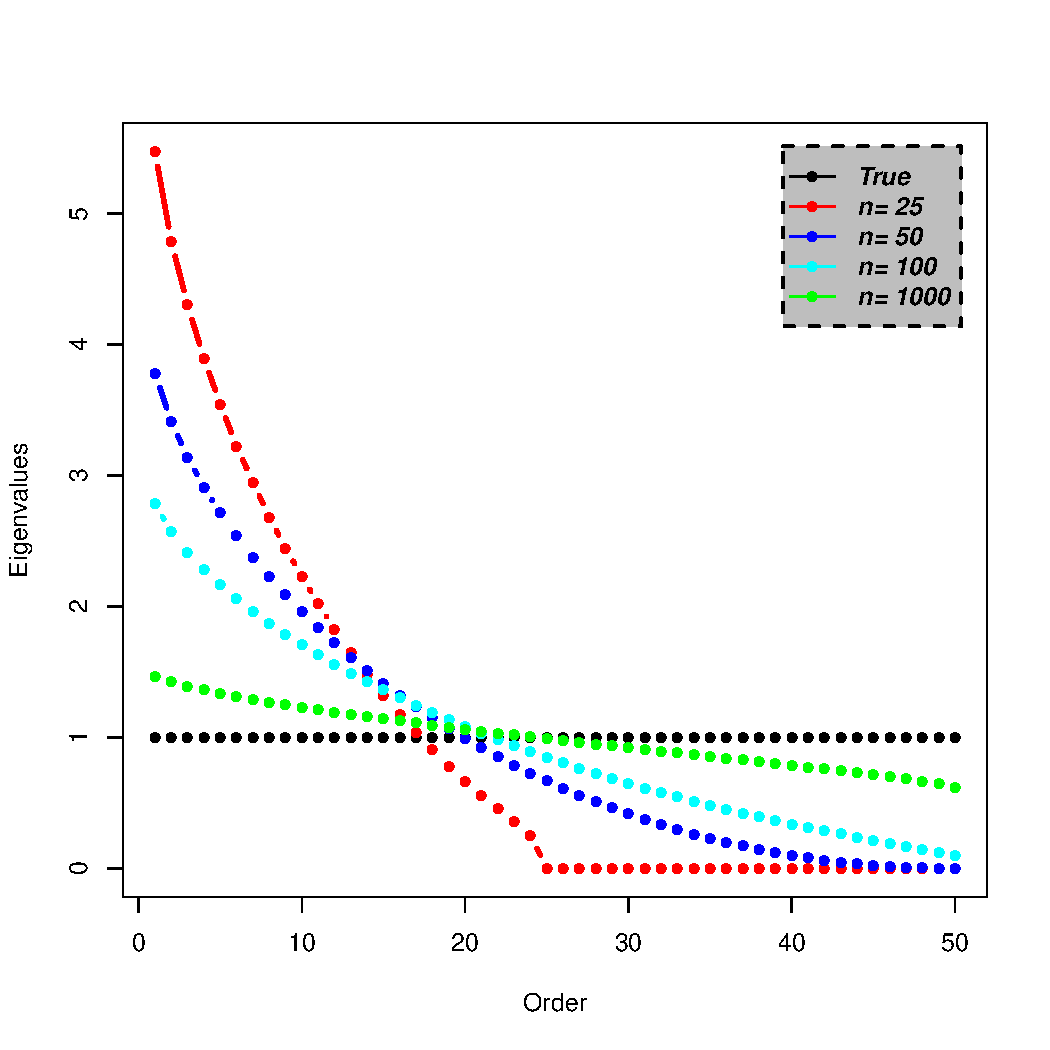
\includegraphics[scale=0.55]{screeplot.pdf}
    		\caption{Sorted eigenvalues of the true and sample covariance matrices for a fixed $p$=50 and $n = \lbrace$25, 50, 100, 1000$\rbrace$ drawn from multivariate normal distribution with Identity matrix as a true covariance matrix.} 
    		\label{Fig1.1}
    	\end{center}
    \end{figure}


%!TEX root = ../thesis.tex
%*******************************************************************************
%****************************** Second Chapter *********************************
%*******************************************************************************

\chapter{Literature review}
\lhead{Chapter 2. \emph{Literature review}}

\newcommand\norm[1]{\left\lVert#1\right\rVert}
\newcommand{\argmax}{\arg\!\max}


\ifpdf
    \graphicspath{{Chapter2/Figs/Raster/}{Chapter2/Figs/PDF/}{Chapter2/Figs/}}
\else
    \graphicspath{{Chapter2/Figs/Vector/}{Chapter2/Figs/}}
\fi


\section{Introduction}

Under a large sample size, the population covariance matrix can be accurately estimated by the sample covariance matrix (maximum likelihood and related unbiased estimator). Consider a vector of random variables, $\textbf{X} = (X_1,X_2, ... ,X_p)$, drawn from a $p$-variate normal distribution with mean vector, $\boldsymbol{\mu}$, and covariance matrix, $\boldsymbol{\Sigma}$. The multivariate probability density function of $\textbf{X}$ can be written as

 \begin{equation}
 f(\textbf{X};\boldsymbol{\mu},\boldsymbol{\Sigma}) = \frac{1}{(2\pi)^\frac{p}{2}\left|\boldsymbol{\Sigma}\right|^\frac{1}{2}} \exp[{-\boldsymbol{(X-\mu)^t \Sigma^{-1} (X-\mu)}}],
  \label{equ2.1}
 \end{equation}
where $\boldsymbol{\left|A\right|}$ represent the determinant of a matrix $\boldsymbol{A}$ and $\boldsymbol{A^t}$ represent the transpose of a matrix $\boldsymbol{A}$. However, in practice, the true covariance matrix is unknown and we estimate it from the sample data. The most common approach is to use an estimate which maximize the following log likelihood function:
\begin{equation}
\log L(\boldsymbol{X};\boldsymbol{\Sigma})= Const - \frac{n}{2} \log \left|\boldsymbol{\Sigma}\right|-\frac{1}{2}\boldsymbol{X^t \Sigma^{-1} X}. 
\label{equ2.2} 
\end{equation}  
 Note that, in equation \ref{equ2.2}, without loss of generality, we assume the mean vector $\boldsymbol{\mu}= \textbf{0}$. After differentiating equation \ref{equ2.2} with respect to $\boldsymbol{\Sigma}$ and equating it to zero, we obtain the maximum likelihood estimate of covariance matrix given by $\widehat{\boldsymbol{\Sigma}}=\frac{1}{n}\boldsymbol{X^t X}$. The related unbiased estimate is given by $\boldsymbol{S=\frac{n}{n-1} \widehat{\Sigma}}$. It is noteworthy that when the number of samples is very large, both estimators become equal. Moreover, these estimators of the covariance matrix have some desirable properties When the sample size is large. First, their eigenvalues are closely related to their population counterpart. Second, both estimators are positive definite matrices so they can be inverted to obtain the estimate of the inverse covariance matrix, $\boldsymbol{\Sigma}^{-1}$.

      
      However, in high-dimensional settings, the classical multivariate techniques which uses the sample covariance matrix or its inverse is a key ingredient either fails to work or becomes unreliable. Because of the two undesirable properties of the sample covariance matrix. First, the sample covariance matrix cannot be inverted. Second, the sample covariance matrix contains a massive amount of an estimation error, which can make considerable adverse impacts on the estimation accuracy \citep{fan2016overview}.
      
       To overcome this problem, a number of methods have been proposed in the literature. One method is the Moore-Penrose generalized inverse proposed by \cite{penrose1955generalized}, which is based on the singular value decomposition (SVD). In high-dimensional data, ($p \gg n$) Moore-Penrose generalized inverse is often used to find the inverse of the sample covariance matrix $\boldsymbol{\hat{\Sigma}}$. To find the inverse of $\boldsymbol{\hat{\Sigma}}$ it is decomposed as $\boldsymbol{\hat{\Sigma}} = \boldsymbol{UDV^{t}}$, where $\boldsymbol{U}$ and $\boldsymbol{V}$ are the matrices of orthonormal eigenvectors and $\boldsymbol{D}$ is the diagonal matrix with diagonal elements equal to the square root of the eigenvalues of $\boldsymbol{\hat{\Sigma}\hat{\Sigma^{t}}}$. Moore-Penrose generalized can be achieved by using the equation
\begin{equation}
\boldsymbol{\hat{\Sigma}^{-1}} = \boldsymbol{VD^{-1}U^{t}},
\label{equ2.3}
\end{equation}       
where all the zero diagonal elements of $\boldsymbol{D}$ and the corresponding eigenvectors in $\boldsymbol{U}$ and $\boldsymbol{V}$ are removed before finding generalized inverse given in equation \ref{equ2.3}. It is interesting to note that Moore-Penrose generalized inverse reduces to the standard matrix inverse whenever $rank$($\boldsymbol{\hat{\Sigma}}$) $\geq p$ \citep{golub1965calculating}. Other regularization procedures closely related to our work are explored in the following sections. 

\section{Shrinkage estimation}   
Historically, the idea of shrinkage estimation is going back to \cite{stein1956inadmissibility} who observed that the estimator can be improved through shrinking towards the structure target. The same idea is used by the \cite{ledoit2004well} who proposed the procedure to find an estimator by the convex combination of the sample covariance matrix and a target matrix. This convex combination is as follows:   
\begin{equation}
\boldsymbol{\hat{\Sigma}_{\gamma}} = \gamma \boldsymbol{T} + (1-\gamma) \boldsymbol{\hat{\Sigma}},
\end{equation}       
where $\boldsymbol{\hat{\Sigma}_{\gamma}}$ is the improved estimator and $\boldsymbol{T}$, $\boldsymbol{\hat{\Sigma}}$ are the target matrix and maximum likelihood estimator of the covariance matrix respectively. They provided a procedure to find shrinkage intensity $\gamma$ by minimizing the expected square loss function, given by          
\begin{equation}
R(\gamma) = E \norm{\boldsymbol{\hat{\Sigma}_{\gamma}} - \boldsymbol{\hat{\Sigma}}}^2,
 \label{equ2.4}
\end{equation}           
where expected square loss function is the measure of mean square error. Interestingly, there is no need to assume that the random variables $p$ follows any specific distribution. But this procedure assumed to exist the first four moments \citep{schafer2005shrinkage}. It can be shown that this improved estimator is well-conditioned \citep{ledoit2004well}.     

\cite{schafer2005shrinkage} followed the same procedure for computing the shrinkage parameter. To compute $\gamma$ minimizing equation \ref{equ2.4} with respect to $\gamma$ we get,
\begin{equation}
\hat{\gamma} = \frac{\sum_{i=1}^{p} \sum_{j=1}^{p} var(\hat{\sigma}_{ij}) - cov(t_{ij}, \hat{\sigma}_{ij})- bias(\hat{\sigma}_{ij}) E(t_{ij} - \sigma_{ij})^{2}}{\sum_{i=1}^{p} \sum_{j=1}^{p} E [t_{ij} - \sigma_{ij}]^{2}},
  \label{equ2.5}
\end{equation}
they described some insights into how the $\gamma$ should be chosen and derived this analytic equation to obtain shrinkage intensity for six commonly used targets for detailed discussion see \citep{schafer2005shrinkage}. Note that if $\boldsymbol{\hat{\Sigma}}$ is an unbiased estimator then equation \ref{equ2.5} reduces to
\begin{equation}
\hat{\gamma} = \frac{\sum_{i=1}^{p} \sum_{j=1}^{p} var(\hat{\sigma}_{ij}) - cov(t_{ij}, \hat{\sigma}_{ij})}{\sum_{i=1}^{p} \sum_{j=1}^{p} E [t_{ij} - \sigma_{ij}]^{2}}.
\end{equation}
Using the identity matrix where all the variables are normalized to have unit variance and its scalar multiple is relatively easy as target $\boldsymbol{T}$ from both analytical and computational perspective. Which is employed by \cite{ledoit2003improved} and \cite{ledoit2004well}. They also demonstrated that the improved estimator is well-conditioned and more accurate than the sample covariance matrix. 

Another target matrix which was the main focus of \cite{schafer2005shrinkage} is the diagonal matrix $\boldsymbol{\hat{\Sigma}_{d}}$ with unequal variances on the main diagonal. This $\boldsymbol{\hat{\Sigma}_{d}}$ only shrinks the eignvalues and keeps the eigenvectors unchanged. In this case $\hat{\gamma}$ is given by
\begin{equation}
\hat{\gamma} = \frac{\sum_{i \neq j}^{p} var(s_{ij})}{\sum_{i \neq j}^{p} E(s_{ij}^2)}.
\end{equation}  
  To compute $\hat{\gamma}$ in this case requares $p$ parameters to be estimated which is complicated as compare to the identity matrix. Note that both identity matrix and $\boldsymbol{\hat{\Sigma}_{d}}$ are positive and sample covariance matrix is the semi-positive definite taking convex combination of one of these targets and sample covariance matrix would result in a positive definite matrix. 

\section{Ridge regularization of the covariance matrix}
As described, in high dimensional settings ($ p \gg n$) the maximum likelihood estimator of the covariance matrix become singular and ill-conditioned. A method so called ridge regularization, proposed by \cite{warton2008penalized} resolve this problem by using 
\begin{equation}
\hat{\boldsymbol{\Sigma}}_{\kappa} = \hat{\boldsymbol{\Sigma}} + \kappa \boldsymbol{I},
\label{risge_est}
\end{equation}
where $\kappa$ is the ridge parameter, $\boldsymbol{I}$ is the $p \times p$ identity matrix and $\hat{\boldsymbol{\Sigma}}_{\kappa}$ is the regularized estimator of the covariance matrix. When the variables are at different scales, it is more appropriate to regularize on the standard scale. In this case \cite{warton2008penalized} regularize the sample estimator of the correlation matrix, $\boldsymbol{R}$, which can be obtained by rescaling equation \ref{risge_est} as 
\begin{equation}
\hat{\boldsymbol{R}}_{\gamma} = \gamma \hat{\boldsymbol{R}} + (1-\gamma) \boldsymbol{I},
\label{corr}
\end{equation}
where $\gamma = \frac{1}{1+\kappa} \in (0,1]$ is the ridge parameter and $\boldsymbol{\hat{R}}_{\gamma}$ is the regularized estimator of the correlation matrix. It is the shrinkage estimator as it shrinks $\boldsymbol{\hat{R}}$ toward the identity matrix and also guaranteed to be a positive definite matrix for any value of $\gamma \in (0,1]$. One interesting property of $\boldsymbol{\hat{R}}_{\gamma}$ is that it can be derived from the penalized likelihood function for multivariate normal data, with penalty term proportional to tr($\boldsymbol{R^{-1}})$ see \citep{warton2008penalized} for analytical derivation. The penalize likelihood function is given by
\begin{equation}
\log L(\boldsymbol{X};\boldsymbol{\Sigma})= Const - \frac{n}{2} \log\left|\boldsymbol{\Sigma}\right|-\frac{1}{2}\boldsymbol{X^t \Sigma^{-1} X} - \frac{c}{2} tr(\boldsymbol{R^{-1}}).
\end{equation}
Using equation \ref{corr} the regularized estimator of $\boldsymbol{\Sigma}_{\gamma}$ can be obtained as
\begin{equation}
\hat{\boldsymbol{\Sigma}}_{\gamma} = \hat{\boldsymbol{\Sigma}}_{d}^{1/2} (\gamma \hat{\boldsymbol{R}} + (1-\gamma) \boldsymbol{I}) \hat{\boldsymbol{\Sigma}}_{d}^{1/2}.
\end{equation}


To estimate regularization parameter $\gamma$, \cite{warton2008penalized} is using $k$-fold cross validation. In this case $k$-fold cross validation is done by dividing the whole sample of size $n$ of a matrix $\textbf{X}$ into $\textbf{k}$ sub-samples denoted by $\textbf{X} = [\textbf{X}_{1}^{T}, \textbf{X}_{2}^{T}, ...,\textbf{X}_{\textbf{K}}^{T}]$. In which the $K$-th sub-samples, that is, $\textbf{X}_{K}$ is used as the validation data and the rest of the observations are used as training data. For example, a total sample size is 20 and we divide it into 5 equal parts in which each sub-sample consist of 4 observations. The training data, $\textbf{X}_{K}$, is used to compute its mean, covariance matrix and correlation matrix denoted by $\boldsymbol{\mu}^{\setminus k}$, $\boldsymbol{\Sigma_{\gamma}}^{\setminus k}$ and $\boldsymbol{R}^{\setminus k}$ respectively. The observed likelihood is then calculated for each $\textbf{X}_{K}$. And then estimate $\gamma$ by maximizing the cross validation likelihood function which is given by

\begin{align}
\begin{split}
-2 \log L(\boldsymbol{\mu}^{\setminus k}, \boldsymbol{\Sigma}^{\setminus k};\boldsymbol{X})= {}& (n_{k}p)  \log(2\pi) + n_{k} \log\left|\boldsymbol{\hat{\Sigma}}_{\gamma}^{\setminus k}\right|  \\ &
+ tr[\boldsymbol{(X_{k}- \boldsymbol{\mu}^{\setminus k}) (\hat{\Sigma}_{\gamma}^{\setminus k})^{-1} (X_{k} - \boldsymbol{\mu}^{\setminus k})}].
\end{split}
\end{align}


To obtain an optimal value of $\gamma$ we use the following equation.

\begin{equation}
\gamma =  \argmax_\gamma \sum_{k=1}^{K} \log L(\boldsymbol{\mu}^{\setminus k}, \boldsymbol{\Sigma}^{\setminus k};\boldsymbol{X_{k}}).
\end{equation} 

\section{Covariance matrix regularization via lasso}
The Inverse of a covariance matrix of the multivariate normal distribution is used to find out conditional independence relationship between two variables given the rest of $p-2$. These conditional dependencies can be visualized graphically called the Gaussian graphical model. However, the population inverse covariance matrix is unknown and we estimate it by the two well known estimators (maximum likelihood estimator and its unbiased version). These two estimators cannot produce estimated elements exactly eqaul to zero, no matter what the sample size is if they are zero in the true covariance matrix. Which makes the model unnecessarily more complex. This complexity and noise of the inverse covariance matrix can be reduced by setting some of the elements equal to zero, a technique called covariance selection proposed by \cite{dempster1972covariance}.  

The lasso regularization was first introduced by \cite{tibshirani1996regression} in the regression context in order to enhance the accuracy and interpretability of the model by setting some of the coefficients exactly equal to zero and shrink important coefficient toward zero. This idea was used by \cite{yuan2007model} and \cite{d2008first} using the penalized log-likelihood method and derived different lasso algorithms for the sparse covariance selection. A fastest algorithm is the graphical lasso algorithm (Glasso) introduced by \cite{friedman2008sparse} for estimating the inverse covariance matrix by applying the lasso penalty. The lasso problem can be solved by using the coordinate decent algorithm \citep{friedman2007pathwise}.  
 
%!TEX root = ../thesis.tex
%*******************************************************************************
%****************************** Third Chapter **********************************
%*******************************************************************************

\chapter{Informative targets and regularization of covariance matrix using informative targets}
\lhead{Chapter 3. \emph{New regularization method}}
\def\tr{\mbox{tr}}


% **************************** Define Graphics Path **************************

\section{Introduction} \label{sec1}
In this chapter, we use the steinian-class shrinkage estimation which is the convex linear combination of the sample covariance matix, $\boldsymbol{\hat{\Sigma}}$, and the target matrix, $\textbf{T}$, given by 
 \begin{equation}
    \hat{\boldsymbol{\Sigma}}_{\gamma}  = \gamma\textbf{T} + (1-\gamma) \hat{\boldsymbol{\Sigma}},
     \label{equ1}
     \end{equation}
where $\gamma  \in [0,1]$ is the shrinkage parameter. The target matrix need to be pre-specified and an appropriate value of $\gamma$ need to be chosen over a grid of values. Note that, when $\gamma=0$ no shrinkage is applied and the sample covariance matrix is retained, and when $\gamma=1$ full shrinkage is applied, which results $\textbf{T}$ as an estimator of the covariance matrix. \cite{ledoit2003improved} and \cite{ledoit2004well} uses identity matrix as a target estimator and the R package "corpcor" specify identity matrix as a target \citep{schaefer2013corpcor}. But sometimes it may not be a good choice as explained by \cite{schafer2005shrinkage}, the identity matrix shrinks all the diagonal and off-diagonal elements of the sample covariance matrix and consequently change the whole eigenstructure of the sample covariance matrix. \cite{schafer2005shrinkage} also discussed the six commonly used targets including identity matrix and their main focus was the diagonal matrix as a target with diagonal elements variances and off-diagonal elements zero pre-assuming that all the variables are independent, which only shrinks the eigenvalues and leave the eigenvectors intact.  

We use two more informative target matrices, that are, first order auto-regressive AR(1) and exchangeable covariance structures for which the correlation parameter, $t \in [0,1]$, is the essential element. We maximize the likelihood function of the multivariate normal distribution to choose an appropriate value of the correlation parameter as described in the next section. Next, we calculate the appropriate value of the shrinkage parameter via maximizing the likelihood function of the multivariate normal distribution. Moreover, we also obtain the optimal shrinkage intensity for the above mentioned targets by minimizing the expected quadratic loss function.    
%We use two more informative target matrices to shrink the sample covariance matrix towards them and calculate the optimal shrinkage intensity by minimizing the expected quadratic loss function. In case of these two targets the optimal shrinkage intensity rely on the correlation parameter, we maximize the likelihood function of the multivariate normal distribution to choose an appropriate value of the correlation parameter as described in the next section. In addition, we use the identity matrix as a target and choose several values of $\gamma$ to obtain the improved estimator via maximizing the likelihood function of the multivariate normal distribution. 

% First, we use the identity matrix as a target and several fixed values of $\gamma$ to obtain the improved estimator via maximizing the likelihood function of the multivariate normal distribution. Second, we use two more informative target matrices to shrink the sample covariance matrix towards them and calculate the optimal shrinkage intensity by minimizing the expected quadratic loss function. In case of these two targets the optimal shrinkage intensity rely on the correlation parameter, we maximize the likelihood function of the multivariate normal distribution to choose an appropriate value of the correlation parameter as described in the next section. 

\section{Estimation of Correlation parameter}

Correlation parameter is the essential element of the two covariance structures, namely AR(1) and exchangeable covariance structures which needs to be estimated. The AR(1) covariance structure can be defined as the first order auto-regressive structure which considers the correlation systematically decreasing with increasing the distance between the time points given by
\begin{equation}
     \sigma_{ij} = t^{|i-j|} \quad     \text{for} \quad  1 \le i,j \le p,
     \label{equ2}
\end{equation}
whereas exchangeable covariance structure can be defined as the matrix with the same covariance between variables and the variances remains constant by rearranging (exchanging) the variables given by
\begin{equation}
\sigma_{ij} = 
\begin{cases}
                                   1 & \text{when $i=j$} \\
                                   t & \text{when $i \neq j$} 
  \end{cases} \quad     \text{for} \quad  1 \le i,j \le p,
  \label{equ3}
\end{equation}
where $t$ is the constant correlation parameter and can be obtained by simply maximizing the $\log$-likelihood function of the multivariate normal distribution for both covariance structures. Let's denote the AR(1) and exchangeable covariance structures by  $\boldsymbol{\Sigma_{t}}$, the $\log$-likelihood function can be written as

 \begin{equation}
 \log L(\boldsymbol{X};\boldsymbol{\Sigma_{t}})= Const - \frac{n}{2} \log\left|\boldsymbol{\Sigma_{t}}\right|-\frac{1}{2}\boldsymbol{X^t \Sigma_{t}^{-1} X}.
 \label{equ4}
 \end{equation}
Differentiating equation \ref{equ4} with respect to $t$ we get
 \begin{equation}
 \frac{\partial}{\partial t} \log L(\boldsymbol{X};\boldsymbol{\Sigma_{t}}) = - \frac{n}{2} \frac{\partial}{\partial t} \log\left|\boldsymbol{\Sigma_{t}}\right|-\frac{1}{2} \tr \big ( \boldsymbol{X^t \frac{\partial}{\partial t} \Sigma_{t}^{-1} X} \big ).
  \label{equ5}
 \end{equation}
  Solving equation \ref{equ5} for AR(1) covariance structure the determinant of $\boldsymbol{\Sigma_{t}}$ is $\boldsymbol{|\Sigma_{t}|} = (1- t^2)^{p-1} $ and the derivative of $\log\left|\boldsymbol{\Sigma_{t}}\right|$ with respect to $t$ gives
  \begin{equation}
  \frac{\partial}{\partial t} \log |\Sigma_{t}|= \frac{-2(p-1)t(1-t^2)^{p-2}}{(1-t^2)^{p-1}}.
  \label{equ6}
  \end{equation}
The inverse of $\boldsymbol{\Sigma_{t}}$ is given by
\begin{equation*}
\Sigma_{t}^{-1}= \frac{1}{(1-t^2)}
  \begin{pmatrix}
    1 & -t & 0 & ... & 0 & 0 \\
    -t & 1+t^2 & -t & ... & 0 & 0 \\
    0 & -t & 1+t^2 & ... & 0 & 0 \\
    \vdots   & \vdots & \vdots &  \vdots &   \vdots & \vdots\\
    0 & 0 & 0 & ... & 1+t^2 & -t  \\
    0 & 0 & 0 & ... & -t & 1 \\
  \end{pmatrix}.
\end{equation*}
The derivative of $ \boldsymbol{\Sigma_{t}^{-1}}$ with respect to $t$ is given by
   \begin{equation*}
\frac{\partial}{\partial t} \Sigma_{t}^{-1}= \frac{1}{(1-t^2)^2}
  \begin{pmatrix}
    2t & -(1+t^2) & 0 & \hdots & 0 & 0 \\
    -(1+t^2) & 4t & -(1+t^2) & \hdots & 0 & 0 \\
    \vdots & \vdots & \vdots & \vdots & \vdots & \vdots \\
    0 & 0 & 0 & \hdots & 4t & -(1+t^2)  \\
    0 & 0 & 0 & \hdots & -(1+t^2) & 2t \\
  \end{pmatrix}.  
  \end{equation*}
To find $\tr \big( X^t \frac{\partial}{\partial t} \Sigma_{t}^{-1} X \big )$ in equation \ref{equ5}, we can write $\boldsymbol{X^t X = n \Sigma}$, where $\boldsymbol{\Sigma}$ is true covariance matrix with entries $\sigma_{ij}, 1 \le i,j \le p$, then
\begin{equation}
\begin{split}
n \, \tr \big ( \frac{\partial}{\partial t} \Sigma_{t}^{-1} \Sigma \big )= &\frac{1}{(1-t^2)^2} [ 2t(\sigma_{11} + 2\sigma_{22} + 2\sigma_{33} + ... + 2\sigma_{(p-1)(p-1)} + \sigma_{pp})]\\
& - t^2(\sigma_{12} + \sigma_{21} + \sigma_{23} + ... + \sigma_{(p-1)(p)} + \sigma_{p(p-1)})\\
& - (\sigma_{12} + \sigma_{21} + \sigma_{23} + ... + \sigma_{(p-1)(p)} + \sigma_{p(p-1)}),
\end{split}
\label{equ8}
\end{equation}
since $\boldsymbol{\Sigma}$ is a symmetric matrix, i.e, $\sigma_{ij}=\sigma_{ji}$ and also diagonal elements are all equal to 1, we can write equation \ref{equ8} as

\begin{equation}
n \, \tr \big ( \frac{\partial}{\partial t} \Sigma_{t}^{-1} \Sigma \big ) =\frac{2}{(1+t^2)^2} [t(p-1) - (t^2 + 1) \sum_{i=2}^{p} \sigma_{(i-1)i}].
\label{equ9}
\end{equation}
Substituting equation $\frac{\partial}{\partial t} \log |\Sigma_{t}|$ and $n \, \tr \big ( \frac{\partial}{\partial t} \Sigma_{t}^{-1} \Sigma \big )$ in equation \ref{equ5} and equating it to zero leads to
%\begin{equation*}
%\begin{split}
%\frac{\partial  L(\boldsymbol{X};\boldsymbol{\Sigma(t)})}{\partial t} =& \frac{2n(p-1)t(1-t^2)^{p-2}}{(1-t^2)^{p-1}} - \frac{2n}{2(1-t^2)^2} \big ( t(p-1)\\
%& - (t^2 + 1) \sum_{i=2}^{p} \sigma_{(i-1)i} \big ) =0,
%\end{split}
%\label{equ10}
%\end{equation*}
 \begin{equation}
 t = \frac{\sum_{i=2}^{p} \sigma_{(i-1)i}}{p-1}.
 \label{equ11}
 \end{equation}
 
If $\boldsymbol{\Sigma_{t}}$ is the exchangeable covariance structure then $|\Sigma_{t}| = (1-t)^{p-1} \lbrace 1+(p-1)t \rbrace$, differentiating $\log |\Sigma_{t}|$ with respect to $t$ gives
 \begin{equation}
    \frac{\partial}{\partial t} \log|\Sigma_{t}| = \frac{(1-t)^{p-1} (p-1) + \lbrace 1+(p-1)t \rbrace (p-1)(1-t)^{p-2}}{(1-t)^{p-1} \lbrace 1+(p-1)t \rbrace},
    \label{equ12}
   \end{equation}
 % \begin{equation}
 %log L(\boldsymbol{X};\boldsymbol{\Sigma_{ex}})= Const - \frac{n}{2} log\left|\boldsymbol{\Sigma_{ex}}\right|-\frac{1}{2}\boldsymbol{X^t \Sigma_{ex}^{-1} X}.
 %\label{equ29}
 %\end{equation}
 %Differentiating equation \ref{equ29} with respect to $t$, gives 
 %\begin{equation}
 %\frac{\partial  L(\boldsymbol{X};\boldsymbol{\Sigma_{ex}})}{\partial t} = - \frac{n}{2} \frac{\partial}{\partial t} log\left|\boldsymbol{\Sigma_{ex}}\right|-\frac{1}{2} tr \big ( \boldsymbol{X^t \frac{\partial}{\partial t} \Sigma_{ex}^{-1} X} \big ) =0,
 %\label{equ30}
 %\end{equation}
in this case the inverse of $\Sigma_{t}$ is
 \begin{equation*}
 \begin{split}
 \Sigma_{t}^{-1}=& \frac{1}{(1-t) \lbrace 1+(p-1)t \rbrace}
  \begin{pmatrix}
    1+t & -t & \hdots & -t  \\
    -t & 1+t & \hdots & -t  \\
    \vdots & \vdots & \vdots & \vdots \\
    -t & -t  & \hdots & 1+t
  \end{pmatrix}\\
&=\frac{1}{(1-t)} \big [\textbf{I} - \frac{t}{ \lbrace 1+(p-1)t \rbrace} \textbf{J} \big ],
  \end{split}
 \end{equation*}
 %\begin{equation}
  %=\frac{1}{(1-t)} \big [\textbf{I} - \frac{t}{(1+(p-1)t)} \textbf{J} \big ],
 %\label{equ13} 
 %\end{equation}
where $\textbf{I}$ is the identity matrix and $\textbf{J}$ is the unit matrix, differentiating $\Sigma_{t}^{-1}$ with respect to $t$ gives 
\begin{equation}
\frac{\partial}{\partial t} \Sigma_{t}^{-1} = \frac{1}{(1-t)^2} \textbf{I} - \Big [ \frac{1}{ \lbrace 1+(p-1)t \rbrace^2 (1-t)} + \frac{t}{\lbrace 1+(p-1)t \rbrace(1-t)^2} \Big ] \textbf{J}.
\label{equ14}
\end{equation}
The 
\begin{equation}
\begin{split}
\tr(\frac{\partial}{\partial t} \Sigma_{t}^{-1} \Sigma) =& \frac{p}{(1-t)^2} - p \big [ \frac{1}{\lbrace1+(p-1)t\rbrace^2 (1-t)} + \frac{t}{\lbrace1+(p-1)t\rbrace(1-t)^2} \big ]\\
& - \big [ \frac{1}{\lbrace1+(p-1)t\rbrace^2 (1-t)} + \frac{t}{\lbrace1+(p-1)t\rbrace(1-t)^2} \big ] \sum_{i \neq j}^{p} \sigma_{ij}.
 \end{split}   
  \label{equ15}
\end{equation}
Substituting the values of $n \, \tr(\frac{\partial}{\partial t} \Sigma_{t}^{-1} \Sigma)$ and $\frac{\partial}{\partial t} \log|\Sigma_{t}|$ in equation \ref{equ5} and equating it to zero leads to
\begin{equation}
t = \frac{\sum_{i \neq j}^{p} \sigma_{ij}}{p(p-1)}.
\label{equ16}
\end{equation}
 

\section{Estimation of regularization parameter using normal likelihood} \label{sec3}
To obtain the regularized estimator of the true covariance matrix, we propose to maximize the multivariate normal likelihood function. Given a random sample of size $n$ from $p$-variate normal distribution with mean vector, $\boldsymbol{\mu=0}$, and covariance matrix, $\boldsymbol{\Sigma}$. The log-likelihood function is
\begin{equation}
\log L(\boldsymbol{X};\boldsymbol{\Sigma})= Const - \frac{n}{2} \log\left|\boldsymbol{\Sigma}\right|-\frac{1}{2}\boldsymbol{X^t \Sigma^{-1} X}. 
\label{equ17} 
\end{equation}
In high-dimensional applications the sample estimator of the covariance matrix is not invertible, we use
\begin{equation}
\boldsymbol{\hat{\Sigma}}_{\kappa} = \boldsymbol{\hat{\Sigma}} + \kappa \boldsymbol{T},
\label{equshr}
\end{equation} 
where $\boldsymbol{T}$ is a positive definite informative target matrix and $\kappa > 0$ is the regularization parameter. The expression in \ref{equshr} incorporates additional information that we may have about the structure of the covariance matrix. If the sample size is very small, $\boldsymbol{\hat{\Sigma}}_{\kappa}$ becomes similar (if not equal) to $\boldsymbol{T}$ that is  
\begin{equation*}
\boldsymbol{T} \approx \boldsymbol{\hat{\Sigma}} + \kappa \boldsymbol{T}.
\end{equation*}
This leads to 
\begin{equation}
\kappa\boldsymbol{T} \approx \boldsymbol{T}-\boldsymbol{\hat{\Sigma}},
\label{equnshr}
\end{equation}
which can be exploited to find the value of $\kappa$ as we do later in this section.

The expression in \ref{equnshr} can also be obtained by assuming that some scaled version of $\boldsymbol{T}$ is the true covariance and replace $\boldsymbol{\Sigma}$ by $(1+\kappa)\boldsymbol{T}$ in equation \ref{equ17}, which then becomes
\begin{equation}
 \log L(\boldsymbol{X};\boldsymbol{\Sigma}_{\kappa}) = Const - \frac{n}{2} \log\left|\boldsymbol{T} + \kappa \boldsymbol{T} \right|-\frac{1}{2}\boldsymbol{X^t \frac{1}{1+\kappa}\boldsymbol{T}^{-1} X}.
 \label{equlik}
\end{equation} 
Differentiating \ref{equlik} with respect to $\kappa$ we get
\begin{equation}
\frac{\partial}{\partial \kappa} \log L(\boldsymbol{X};\boldsymbol{\Sigma}_{\kappa}) = - \frac{n}{2} (\boldsymbol{T} + \kappa \boldsymbol{T})^{-1} \boldsymbol{T} + \frac{1}{2} (\boldsymbol{T} + \kappa \boldsymbol{T})^{-1} X^t  X (\boldsymbol{T} + \kappa \boldsymbol{T})^{-1},
\label{equ18}
\end{equation}
where $\frac{\partial}{\partial \boldsymbol{\kappa}} \log |\boldsymbol{A}| = \frac{1}{|\boldsymbol{A}|} |\boldsymbol{A}| \boldsymbol{A}^{-t}$ and $\frac{\partial}{\partial \boldsymbol{\kappa}} \boldsymbol{A}^{-1} = -\boldsymbol{A}^{-1} \frac{\partial A}{\partial \boldsymbol{\kappa}} \boldsymbol{A}^{-1}$. Equating equation \ref{equ18} to zero leads to
\begin{equation*}
 \kappa \boldsymbol{T} = \boldsymbol{S} - \boldsymbol{T},
\end{equation*}
which is similar to the expression in \ref{equnshr} up to a sign which does not make difference when we ignore the sign (take the absolute) as we do in what follows.
Taking $\norm{.}_{1}$ on both sides which is the sum of the absolute of all entries of the matrix, we have
\begin{equation}
 \norm{\kappa \boldsymbol{T}}_{1} = \norm{\boldsymbol{S} - \boldsymbol{T}}_{1},
\label{equ19}
\end{equation}
If target $\boldsymbol{T}$ is the identity matrix then the value of $\kappa$ becomes
\begin{equation}
\kappa = \frac{\norm{\boldsymbol{S} - \boldsymbol{I}}_{1}}{p},
\end{equation}
for AR(1) covariance structure as a target $\kappa$ is
\begin{equation}
\kappa = \frac{\norm{\boldsymbol{S} - \boldsymbol{T}}_{1}}{p + 2\sum_{k=0}^{p-1} kt^{p-k}},
\end{equation}
furthermore, if target $\boldsymbol{T}$ is the exchangeable covariance structure then
\begin{equation}
\kappa = \frac{\norm{\boldsymbol{S} - \boldsymbol{T}}_{1}}{p + p(p-1)t}.
\end{equation}

In order to restrict the range of the regularization parameter between zero and one, it is more appropriate to use the correlation scale rather than the covariance scale in equation \ref{equ19}. The correlation matrix can be obtained as 
\begin{equation*}
\boldsymbol{\hat{R}} = \boldsymbol{\hat{\Sigma}_{d}^{-\frac{1}{2}}} \boldsymbol{\hat{\Sigma}} \boldsymbol{\hat{\Sigma}_{d}^{-\frac{1}{2}}},
\end{equation*}
where $\boldsymbol{\hat{\Sigma}_{d}}$ is the diagonal matrix with corresponding diagonal elements of  $\boldsymbol{\hat{\Sigma}}$. To get the regularization parameter at correlation scale we follow \cite{warton2008penalized} who rather regularized the correlation matrix (not the covariance matrix) and rescale $\kappa$ as
 \begin{equation}
 \gamma = \frac{1}{1+\kappa},
 \end{equation}
where $\gamma \in [0,1]$. The corresponding regularized estimator of the correlation matrix can be obtained as
\begin{equation}
\boldsymbol{R}_{\gamma} = \gamma \boldsymbol{\hat{R}}  + (1-\gamma) \boldsymbol{T}.
\end{equation}

\subsection{Sample properties of $\boldsymbol{\gamma}$}
We present some useful properties of the penalty term $\gamma$. First, for a fixed $p$ as $n$ increases $\gamma$ on the average decreases which indicates that the regularized estimator, $\boldsymbol{\Sigma}_{\gamma}$, is the consistent estimator of the true covariance matrix. In contrast, as $p$ increases the penalty term also decreases and give more weight to the target matrix. Second, for a fixed value of $p$ as we $n$ increases the variance of $\gamma$ tends to decrease.

 For making the above properties of $\gamma$ clear, we conduct a simulation study. We draw a sample of size $n= \lbrace 10,30,300 \rbrace$ from multivariate normal distribution with $p= \lbrace 10, 30, 100 \rbrace$ and mean vector, $\boldsymbol{\mu=0}$, and three types of $\boldsymbol{\Sigma}$, that is, the first order auto-regressive AR(1) covariance structure, exchangeable covariance structure and identity matrix. For both AR(1) and exchangeable covariance structures we consider $t=0.5$ and For each combination of $n$ and $p$ we simulate the data 1000 times and compute penalty parameter $\gamma$ for each combination of $n$ and $p$. Note that we use three types of targets mentioned in section \ref{sec3} in case of AR(1) and exchangeable covariance structures as a target, $\gamma$ depends on the correlation parameter $t$, which we estimate using \ref{equ11} and \ref{equ16} also note that the the penalty term changes with changing the target matrix. The aforementioned properties can be clearly seen in Figure \ref{Fig3.1}.
 


\begin{figure}[h]
\begin{center}$
\begin{array}{ll}
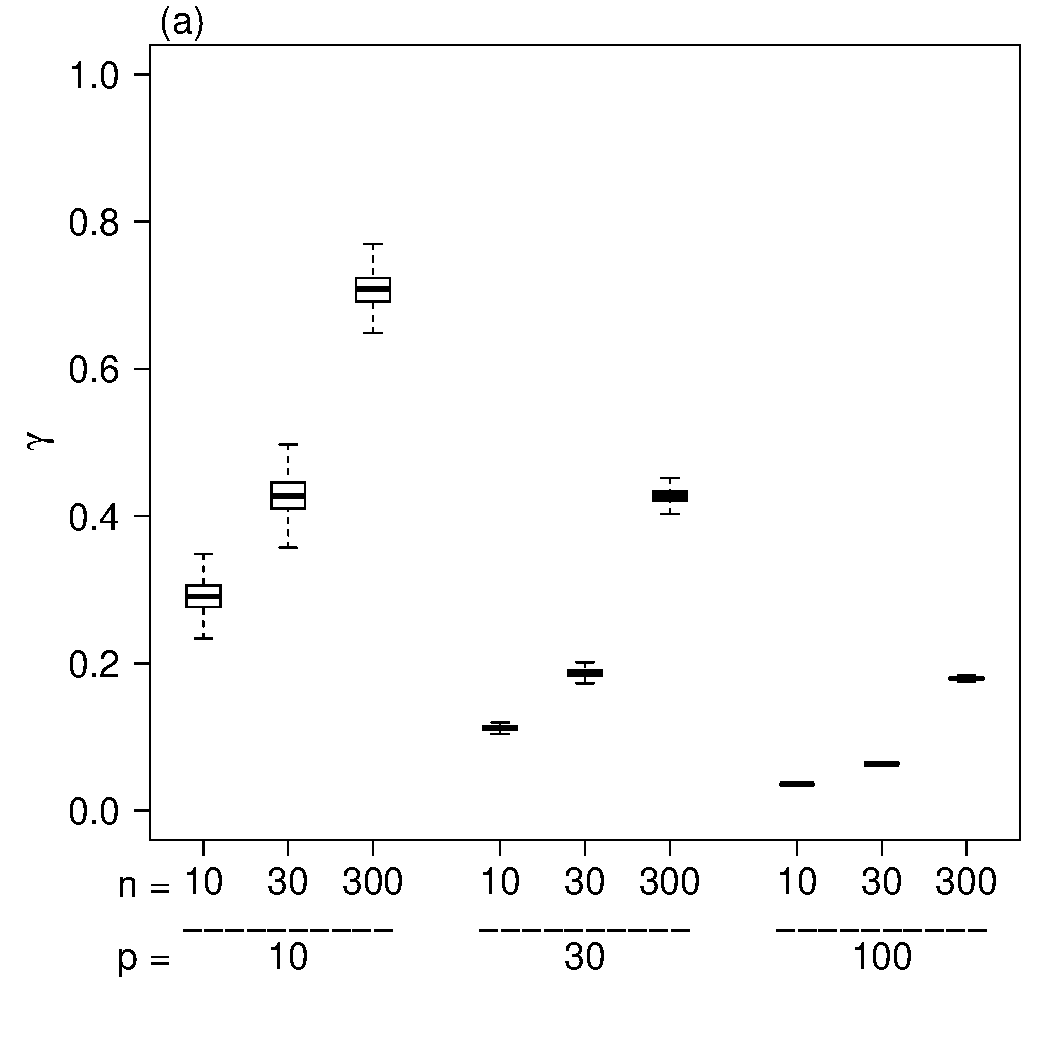
\includegraphics[scale=0.42]{boxId.pdf}
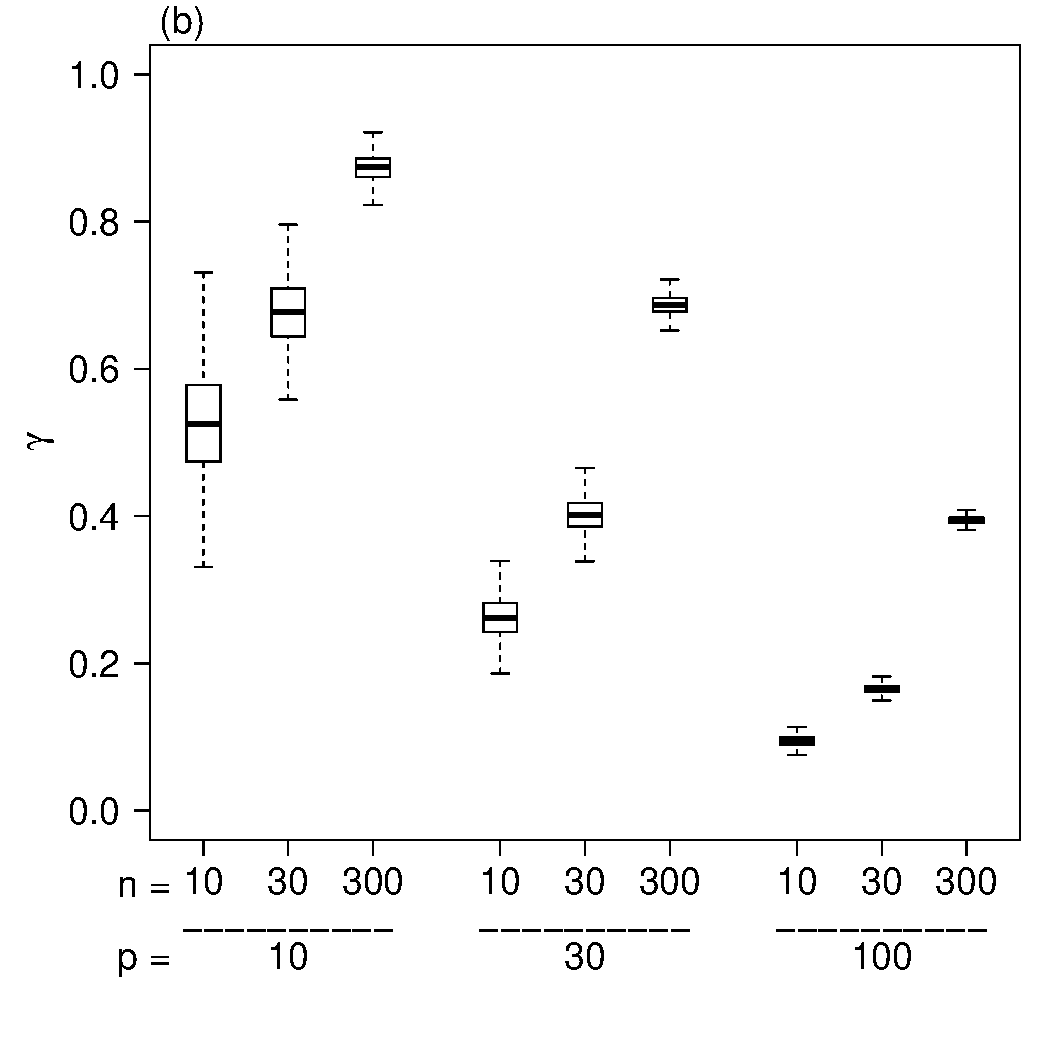
\includegraphics[scale=0.42]{boxAR.pdf}
\end{array}$
\end{center}

\begin{center}$
\begin{array}{r}
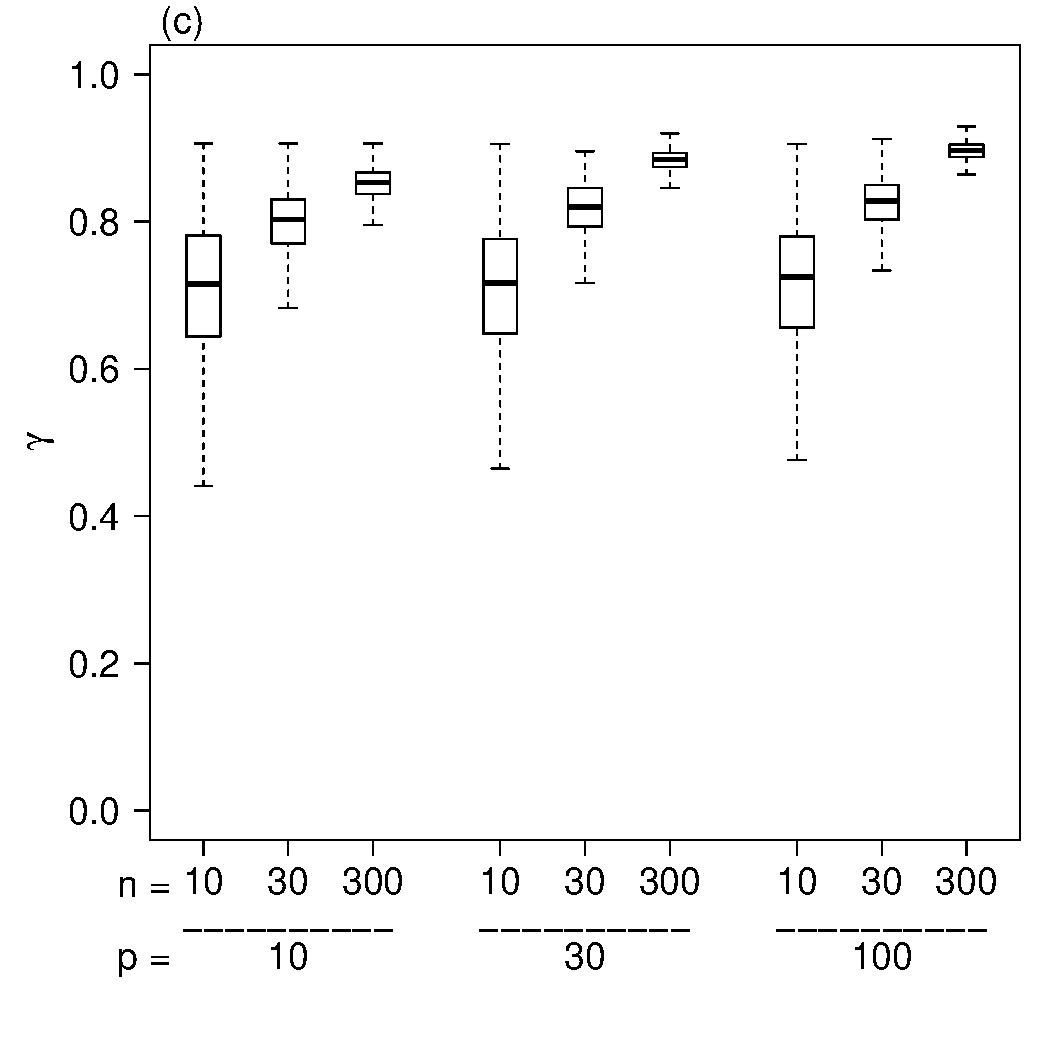
\includegraphics[scale=0.42]{boxex.pdf}
\end{array}$
\end{center}
\caption{Distribution of $\gamma$ values for different samples of size $n= \lbrace 10,30,300 \rbrace$ from a multivariate normal distribution with $p= \lbrace 10, 30, 100 \rbrace$ for different choices of $\boldsymbol{\Sigma}$ simulated 1000 times. (a) identity matrix as a true covariance matrix and as target (b) AR(1) structure as a true covariance matrix and as a target (c) exchangeable structure as a true covariance matrix and as a target.}
\label{Fig3.1}
\end{figure}
\chapter{Simulation study}
\lhead{Chapter 4. \emph{Simulation study}}



\section{Introduction}
In this chapter, we conduct extensive simulation study to numerically demonstrate the performance of the proposed method and also compare it with the shrinkage method proposed by \cite{schafer2005shrinkage} which is also implemented in R package ``corpcor'' \citep{schaefer2013corpcor}.

\section{Synthetic experiments}
To examine the behavior of the proposed method under different simulation settings, we generate various datasets taking into account a number of different parameters. These parameters include varying sample sizes, number of variables, and different covariance structures.

We draw a sample of size $n$ from a $p$-variate normal distribution with mean vector, $\boldsymbol{\mu=0}$, and covariance matrix, $\boldsymbol{\Sigma}$. In order to evaluate the performance in a variety of situations, we consider three different covariance structures for $\boldsymbol{\Sigma}$. These include AR(1) covariance structure given by 
\begin{equation*}
     \sigma_{ij} = t^{|i-j|} \quad     \text{for} \quad  1 \le i,j \le p \quad \& \quad t \in[0,1],
\end{equation*}
the exchangeable coavraince structure given by
\begin{equation*}
\sigma_{ij} = 
\begin{cases}
                                   1 & \text{when $i=j$} \\
                                   t & \text{when $i \neq j$} 
  \end{cases} \quad     \text{for} \quad  1 \le i,j \le p \quad \& \quad t \in[0,1],
\end{equation*}
and the covariance matrix generated by the algorithm presented in \cite{schafer2004empirical}, which we will refer to random structure in the rest of the thesis. The random covariance structure is guaranteed to be a positive definite and allows to control for the number of zeros and the non-zeros entries in the off-diagonal positions of the inverse covariance matrix. Note that the off-diagonal entries of the inverse covariance matrix are the partial covariances and are interpretable in the context of Gaussian graphical models \citep{dempster1972covariance}. The algorithm to generate this covariance matrix is as follows:
\begin{itemize}
\item Start with an empty $p \times p$ matrix.
\item Select randomly a suitable number of off-diagonal positions and fill it with random numbers drawn from uniform distribution between -1 and 1.
\item Set the diagonal elements equal to the absolute sum of the columns of matrix generated in step 2 plus a small positive constant to ensure positive definiteness. This gives us the inverse covariance matrix.
\item The inverse of the matrix obtained in step-3 is the desired covariance matrix. 
\end{itemize}  
For instance, to generate a coavriance matrix whose inverse is sparse we fill only a small proportion of non-zero random numbers in the off-diagonal positions of the inverse covariance matrix. On the other hand filling all the off-diagonal positions with non-zero entries will result in a covariance matrix whose inverse is dense. Furthermore, the inverse of the AR(1) covariance structure is spares and the inverse of the exchangeable covariance structure is dense. These three covariance structures allows to test the method in a range of situations.  

 
We use the following three diffenet matrics to compare the accuracy of the proposed method with the maximum likelihood estimate and the shrinkage method of \cite{schafer2005shrinkage}:
 \begin{itemize}
 \item[1.] Sum of absolute errors in estimated eigenvalues.
 \item[2.] Sum of element-wise squared errors of the estimated covariance matrices.
 \item[3.] Visual comparison of estimated and true eigenvalues.
 \end{itemize}
   
In our first type of experiments, we show the results for $n=50$ and $p=  30, 50, 100$ to demonstrate the effect of increasing number of variables for a fixed value of $n$. The data is simulated from multivariate normal distribution using all three covariance structures mentioned above. For AR(1) and exchangeable covariance structures, we shrink the estimated covariance matrix towards the correct targets that are, respectively, AR(1) and exchangeable. We also examine the performance in which case the target is incorrectly specified as AR(1) and exchangeable while the true covariance matrix is identity. However, for random covariance structure we use only identity matrix as a target, which although is incorrect but have been used extensively as a shrinkage target to regularize the covariance matrix \cite{ledoit2003improved, schafer2005shrinkage}. Note that although we have conducted the experiments for a range of values of $t$, we show here the results only for $t=0.5$ for both AR(1) and exchangeable structures. Similarly, for random covariance structure we show results for a covariance matrix whose inverse contains 30\% of the off-diagonal positions as being non-zero. 

The covariance matrix is estimated using the proposed method and shrinkage method of \cite{schafer2005shrinkage}. For the proposed method whenever the target is correctly specified we estimate $t$ using Gaussian estimating equations as described in chapter 3. Note that the target is correctly specified (but not always) only when we use AR(1) and exchangeable covariance structures. The sum of absolute errors in estimated eigenvalues averaged over 1000 simulated datasets are presented in Figure \ref{Fig1}. The eigenvalues of sample covariance are also plotted not only for comparison purpose but also as a warning that how much our analysis can be unreliable under a high-dimensional setting.

\section*{Results:}
From the simulation results, it is clear that whenever the target is correctly specified in case of both AR(1) and exchangeable covariance structures, the proposed method performs better than the shrinkage method as it maintains the smallest estimation error and is also much precise than the competing methods. Moreover, as $p$ increases the estimates obtained by using the proposed method becomes more accurate and precise. Its performance becomes slightly weaker than the shrinkage method if the target is incorrectly specified as AR(1) or exchangeable while the true true covariance matrix is identity matrix. In case of random covariance structure when we use the identity matrix as a target, our proposed method also outperform than the shrinkage method in terms of accuracy and precision. 

\begin{figure}[H]
\begin{center}$
\begin{array}{ll}
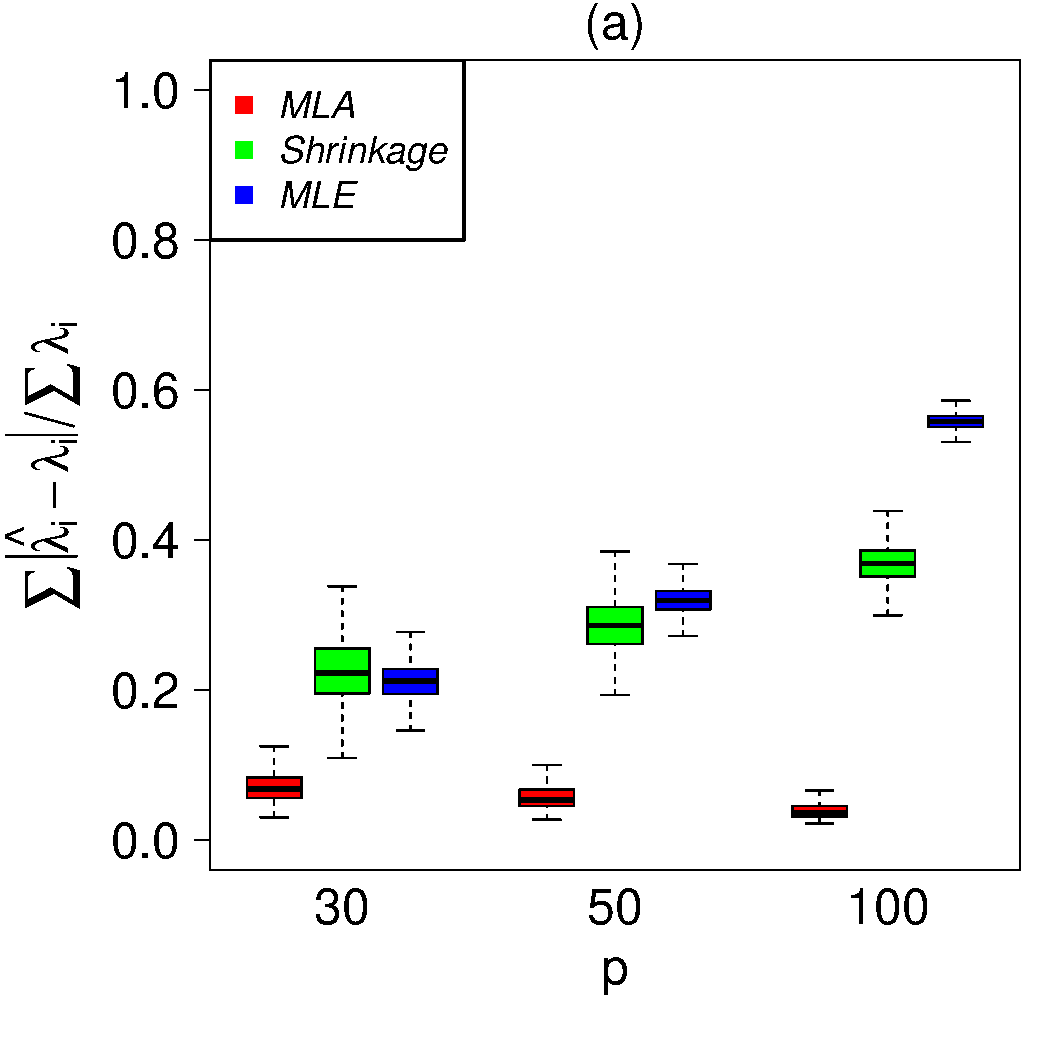
\includegraphics[scale=0.33]{FIG4_2a.pdf}
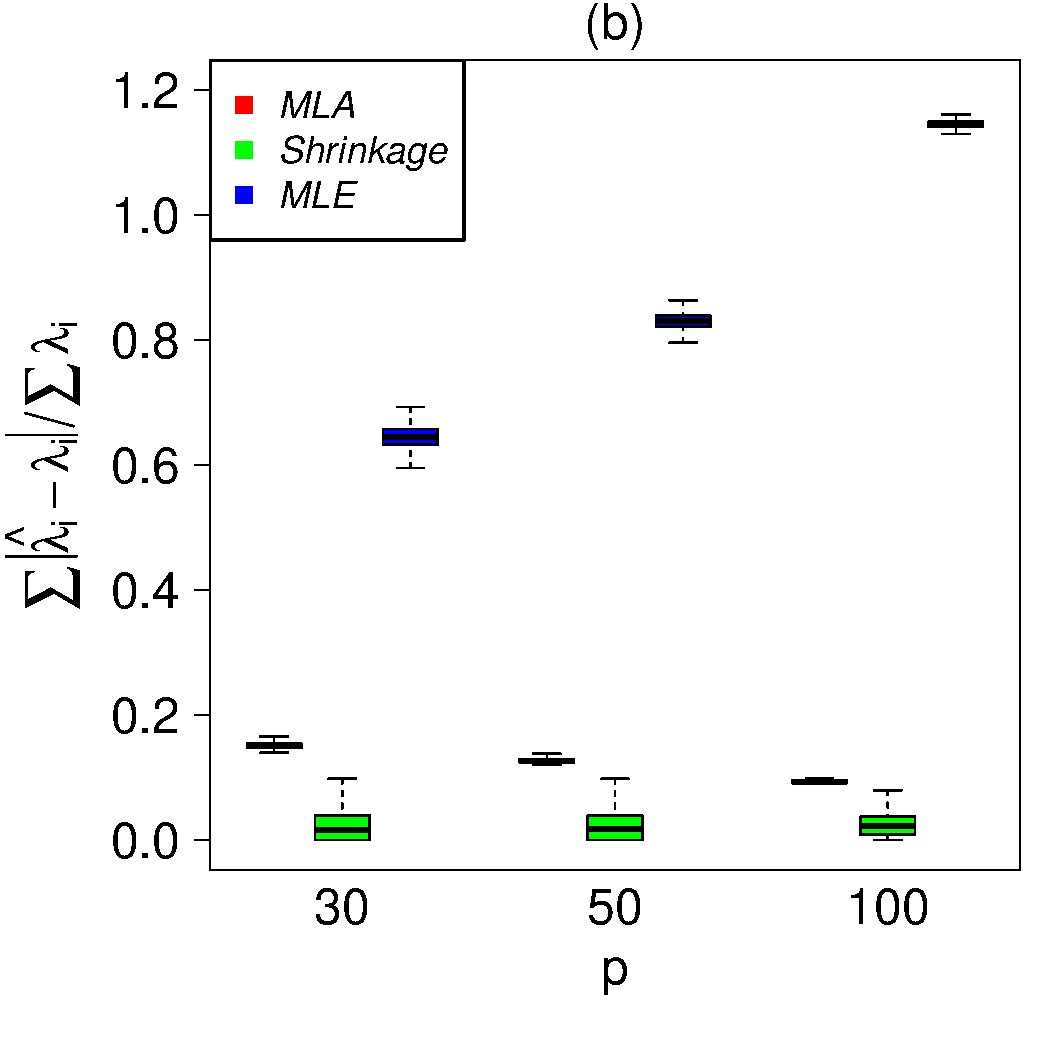
\includegraphics[scale=0.33]{FIG4_2b.pdf}
\end{array}$
\end{center}
\begin{center}$
\begin{array}{ll}
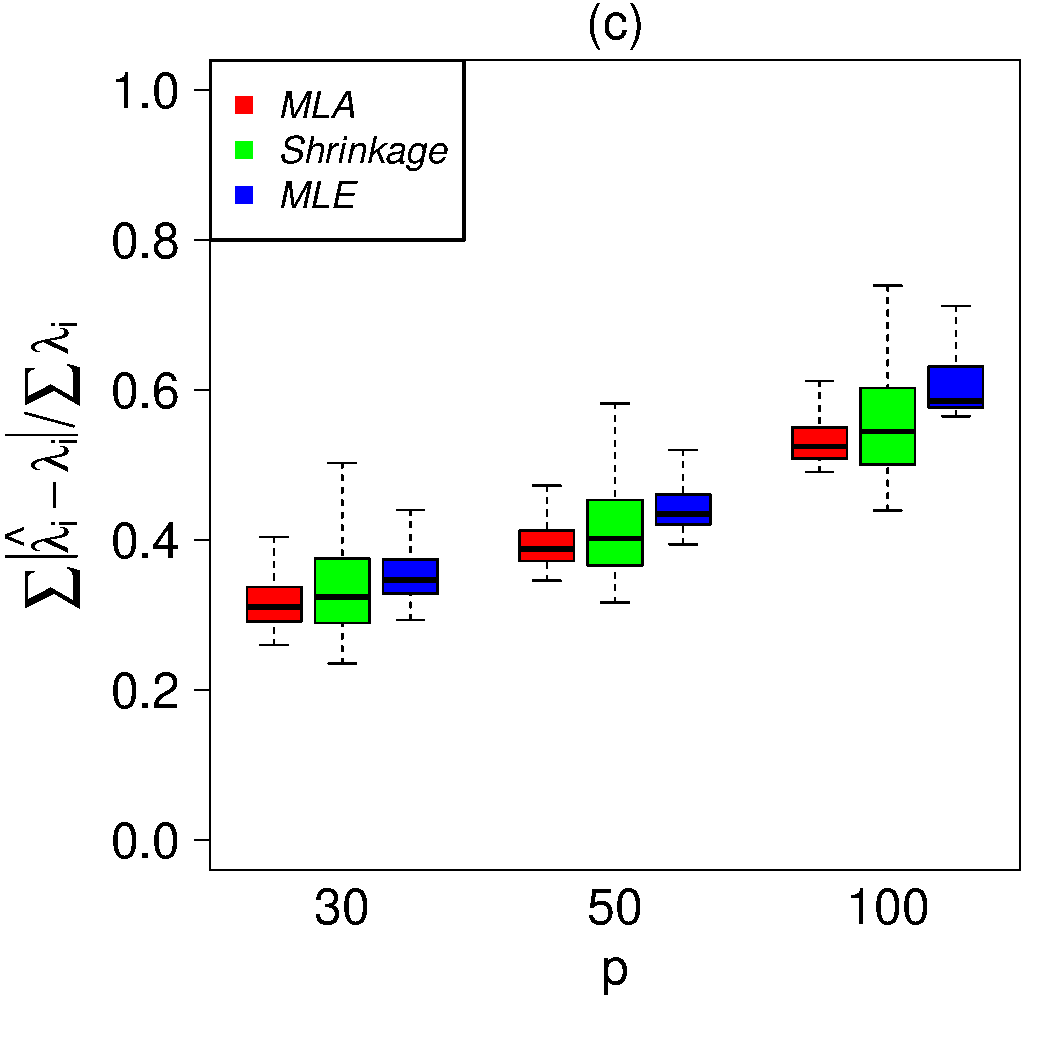
\includegraphics[scale=0.33]{FIG4_2c.pdf}
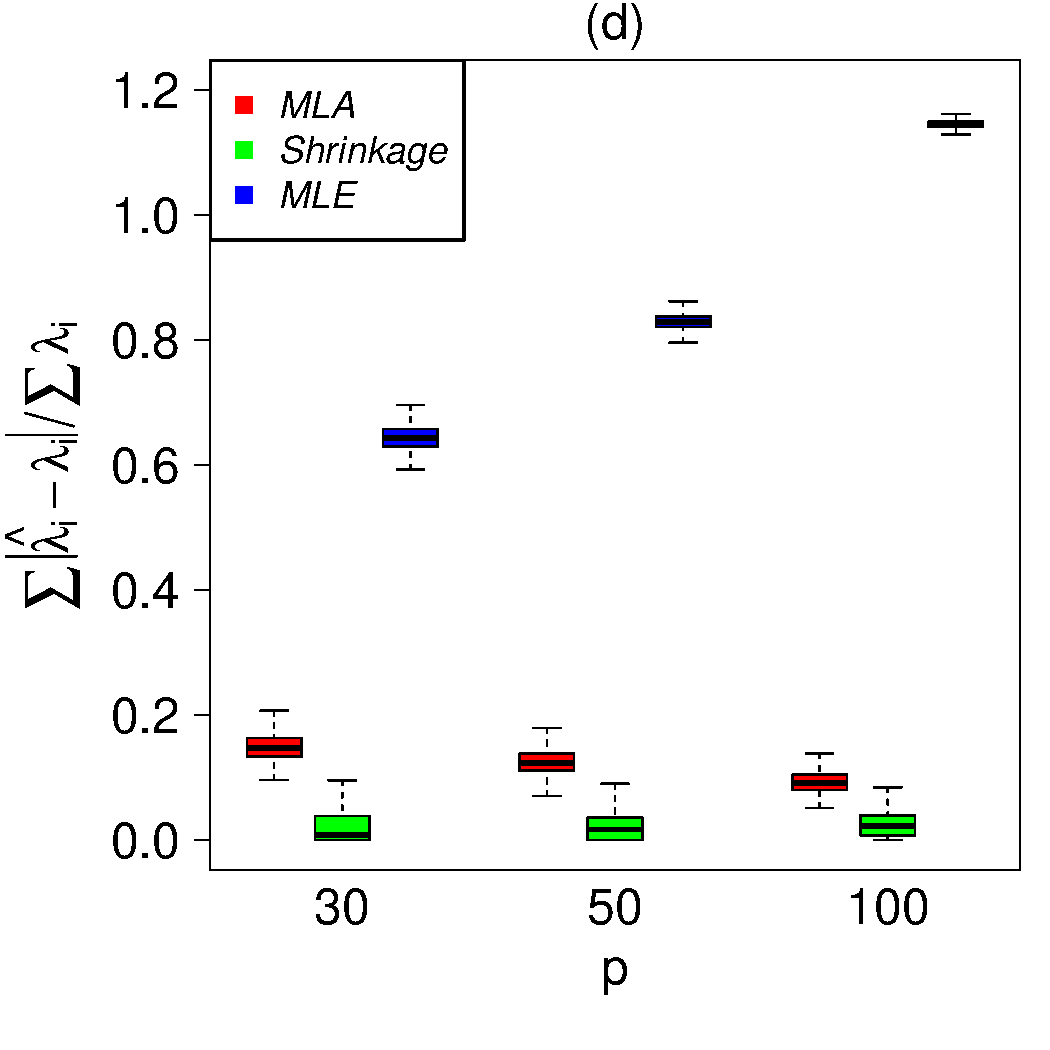
\includegraphics[scale=0.33]{FIG4_2d.pdf}
\end{array}$
\end{center}
\begin{center}$
\begin{array}{r}
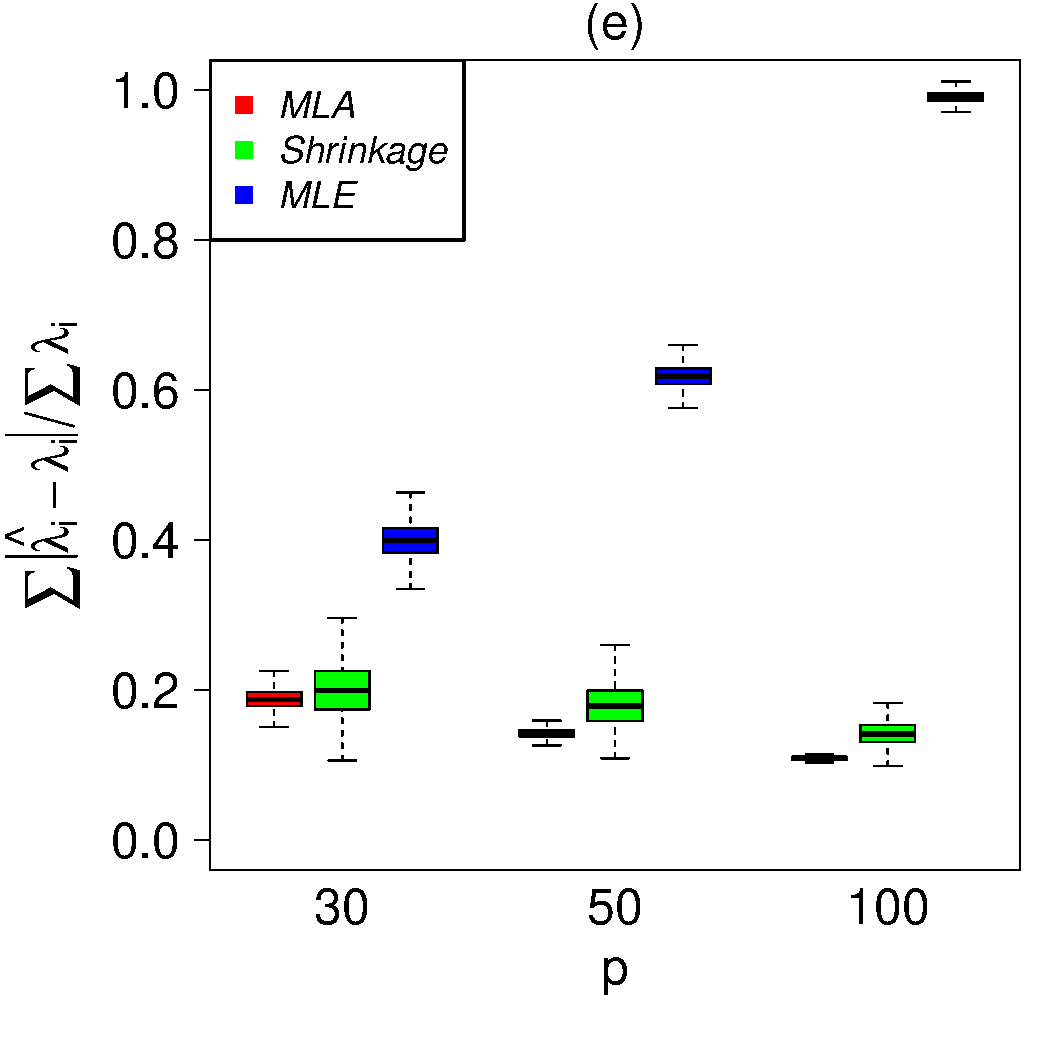
\includegraphics[scale=0.33]{FIG4_2e.pdf}
\end{array}$
\end{center}
\caption{Distribution of the sum of absolute errors in estimated eigenvalues simulated 1000 times using proposed, shrinkage and maximum likelihood methods under different choices of covariance matrices (a, b) AR(1) with $t=0.5$ and identity as true covariance matrix for all three methods and AR(1) as a target for the proposed method (c, d) exchangeable with $t=0.5$ and identity as true covariance matrix for all three methods and exchangeable as a target for the proposed method (e) random covariance structure with 30\% off-diagonal entries as non-zero and identity matrix as a target. The data are generated from multivariate normal distribution with $n=50$ and $p=\lbrace 30,50,100\rbrace$.}
\label{Fig1}
\end{figure}

%\begin{figure}[h]
%\centering
%\begin{subfigure}[t]{.4\textwidth}
%\centering
%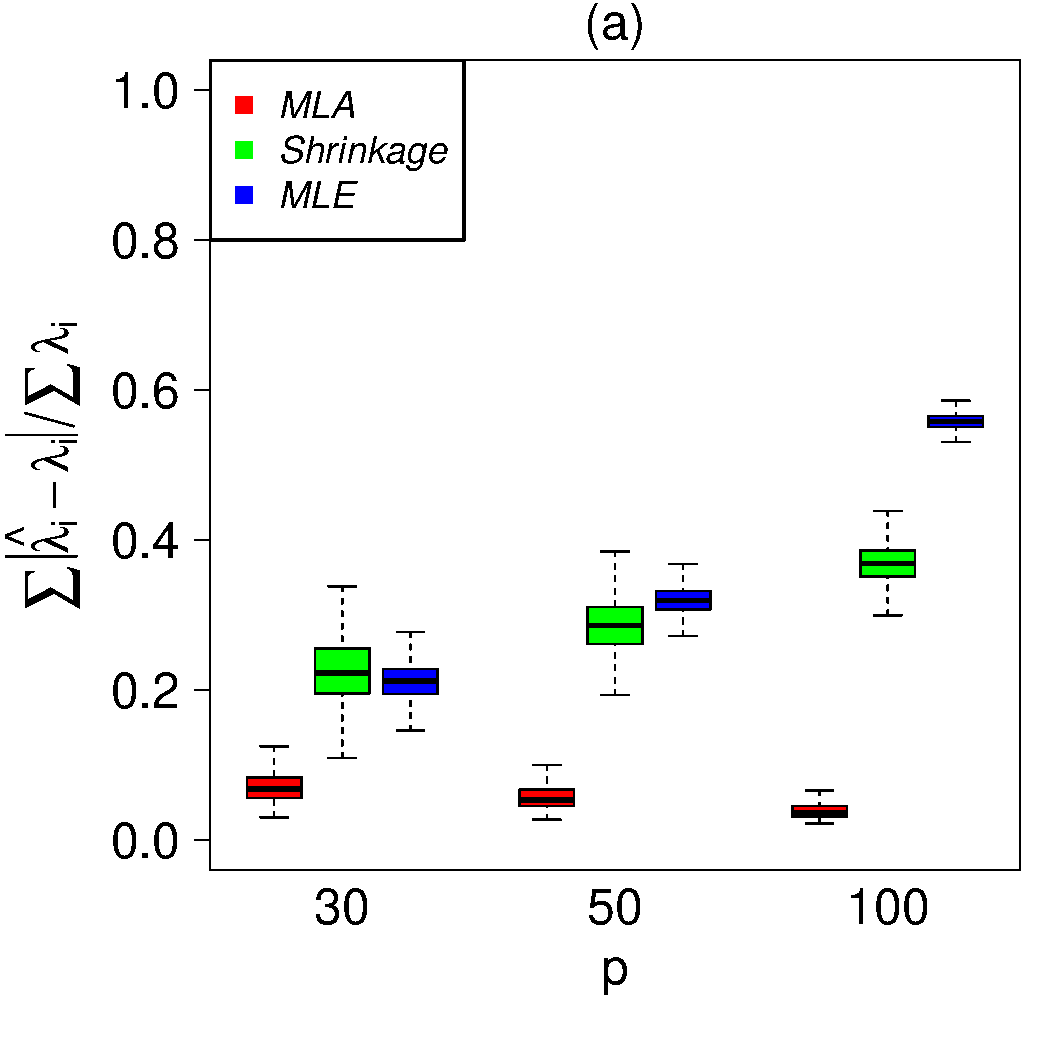
\includegraphics[width=\linewidth]{FIG4_2a.pdf}
%\end{subfigure}
%\begin{subfigure}[t]{.4\textwidth}
%\centering
%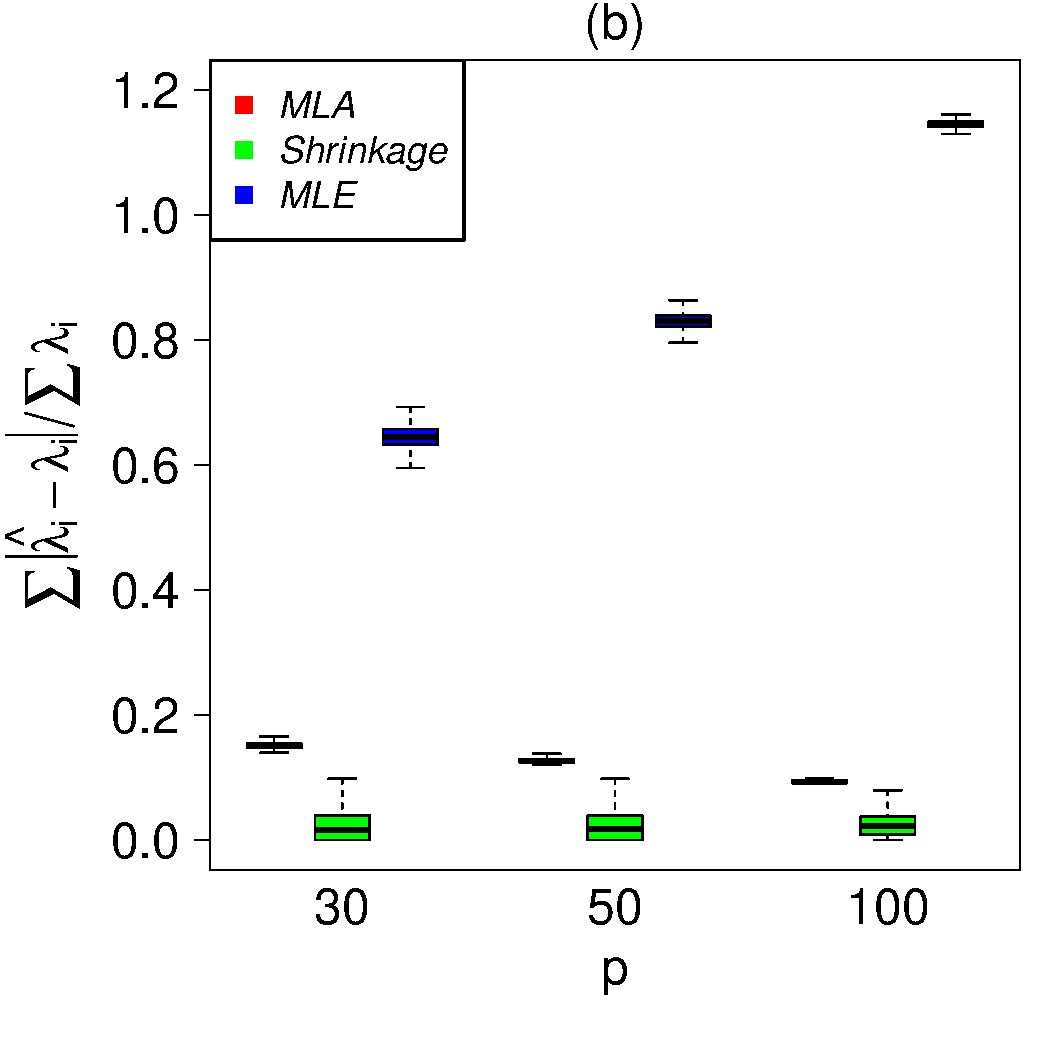
\includegraphics[width=\linewidth]{FIG4_2b.pdf}
%\end{subfigure}
%\medskip
%\begin{subfigure}[t]{.4\textwidth}
%\centering
%\vspace{0pt}
%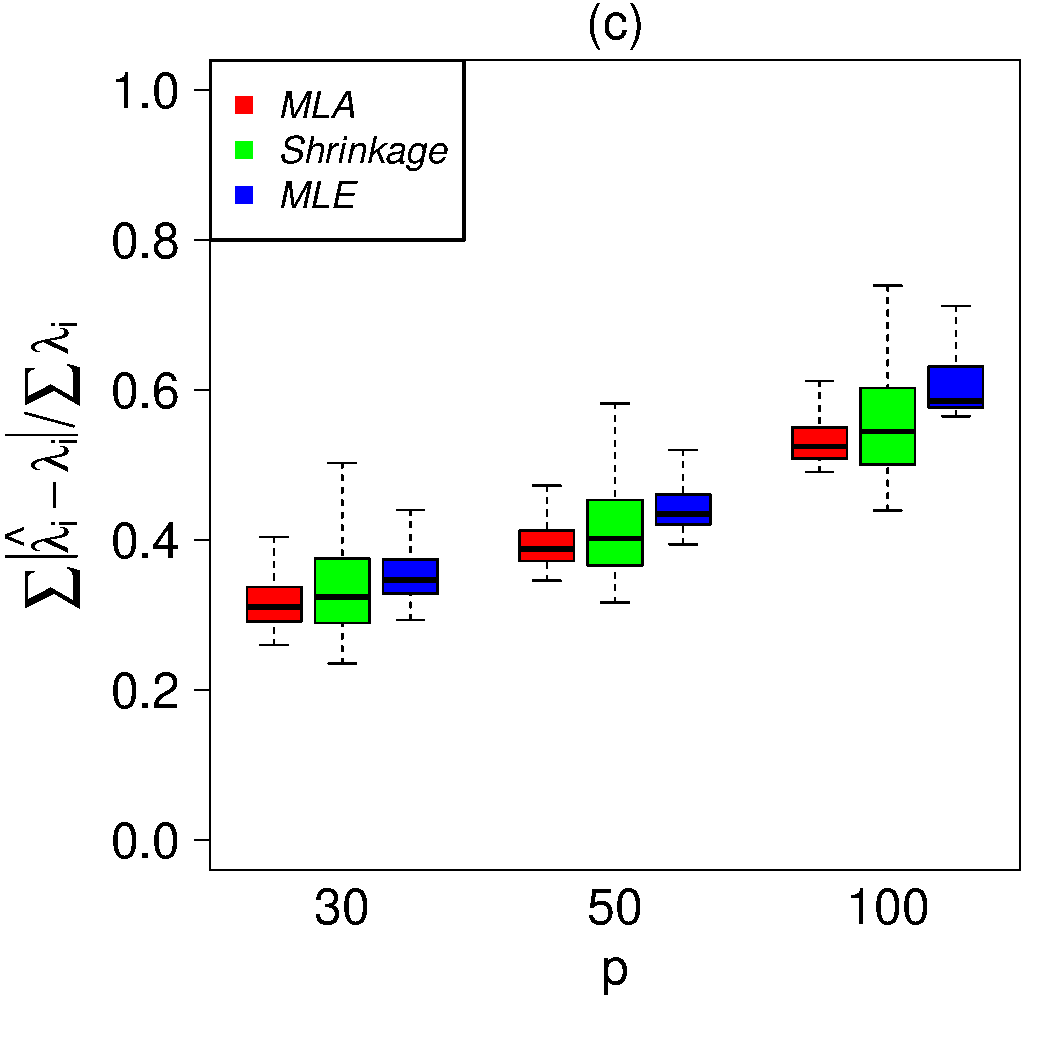
\includegraphics[width=\linewidth]{FIG4_2c.pdf}
%\end{subfigure}
%\begin{subfigure}[t]{.4\textwidth}
%\centering
%\vspace{0pt}
%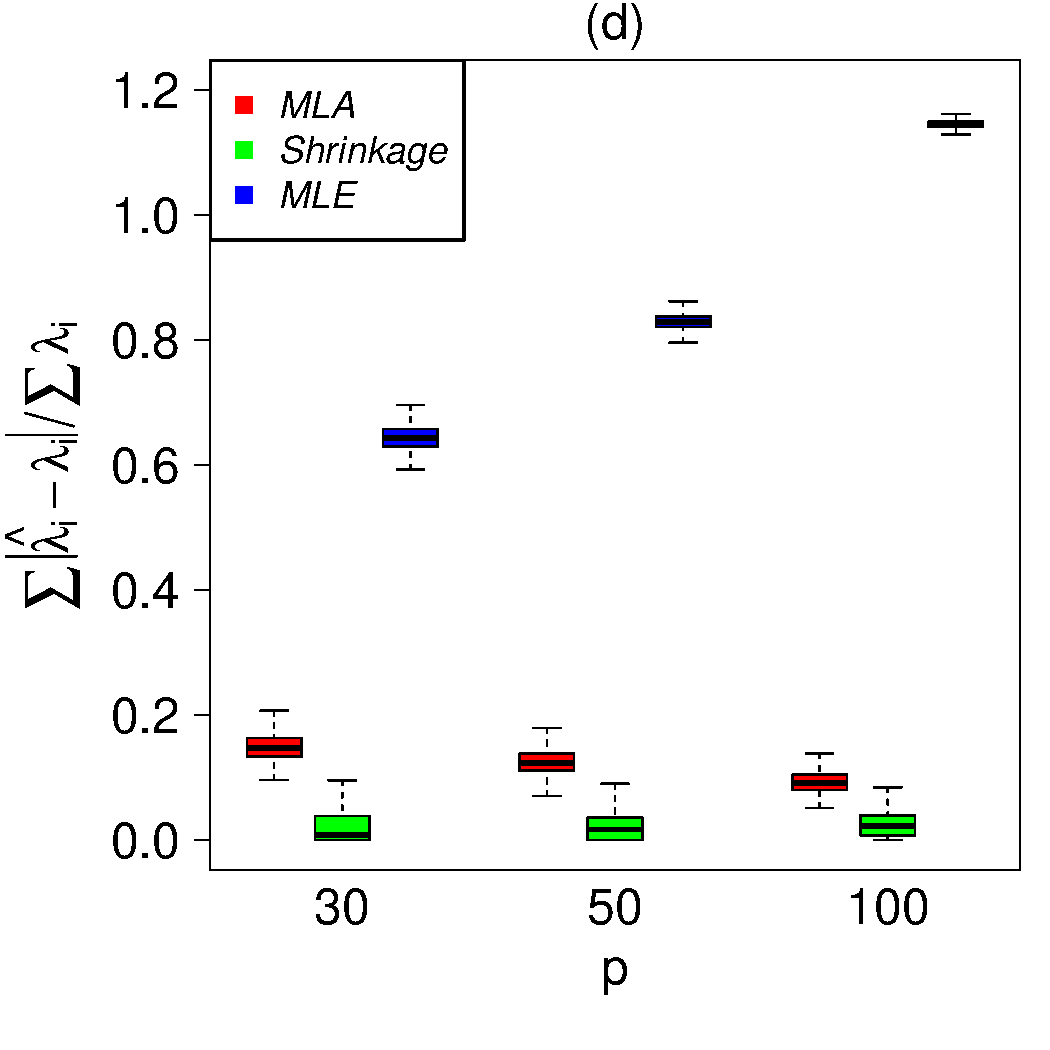
\includegraphics[width=\linewidth]{FIG4_2d.pdf}
%\end{subfigure}
%\begin{subfigure}[t]{.4\textwidth}
%\centering
%\vspace{0pt}
%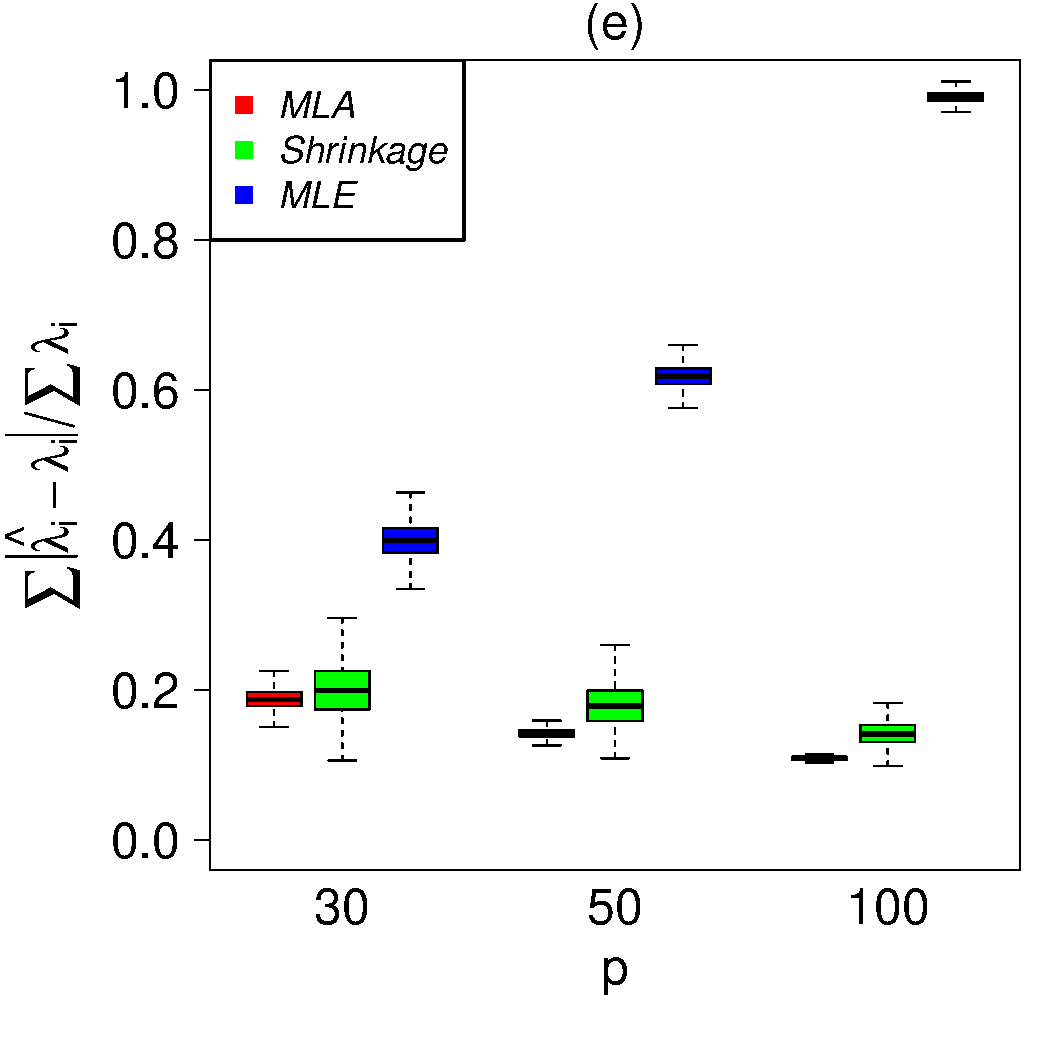
\includegraphics[width=\linewidth]{FIG4_2e.pdf}
%\end{subfigure}
%\caption{Distribution of the sum of absolute errors in estimated eigenvalues simulated 1000 times using proposed, shrinkage and maximum likelihood methods under different choices of covariance matrices and targets for the proposed method arranged in Table \ref{Tab1}. For random covariance structure we took 30\% of the off-diagonal entries as non-zero. The data are generated from multivariate normal distribution with $n=50$ and $p=\lbrace 30,50,100\rbrace$.}
%\label{Fig1}
%\end{figure}
%(a, b) AR(1) covariance structure, (c, d) exchangeable covariance structure, (c) random covariance matrix with $30\%$ proportion on non-zero off-diagonal elements for sample of size $n=50$ from a multivariate normal distribution with $p=\lbrace 30,50,100\rbrace$. These results are simulated 1000 times.
%We use the same covariance structures with parameter values to simulate the data from multivariate normal distribution and with the same targets as was used in the first experiment.
%If the true covariance matrix is AR(1) or exchangeable covariance structure, in that instances we shrink the sample covariance matrix towards two targets: a correct target that is, respectively, AR(1) and exchangeable and incorrect target: identity matrix

For the second type of experiments, we show the results for increasing value of $n= 10,20,30,40,50,60,70,90,120,200$ while keeping $p=10$. In this case we show the asymptotic performance of the competing methods. We use all three aforementioned covariance structures and simulate the data from multivariate normal distribution as we did in the previous case. For this case, we also consider $t=0.5$ for both AR(1) and exchangeable covariance structures and for random covariance structure we take 30\% non-zero off-diagonal elements. When the true covariance matrices are AR(1) and exchangeable we shrink the sample covariance matrix, respectively, towards AR(1) and exchangeable targets, which are correct targets for AR(1) and exchangeable covariance structures. For identity as a true covariance matrix we also use both AR(1) and exchangeable targets to shrink the sample covariance matrix towards them, which is incorrect. In case of random covariance structure we shrink the sample covariance matrix towards the identity matrix (commonly used target to regularized sample covariance matrix whenever $p \gg n$). We then calculate sum of element-wise squared errors (denoted by MSE in the rest of the thesis) of the estimated covariance matrices given by $ \norm{\boldsymbol{\hat{\Sigma}} - \boldsymbol{\Sigma}}_{F}^{2}$, 
%\begin{equation*}
%L(\boldsymbol{\hat{\Sigma}}, \boldsymbol{\Sigma}) = \norm{\boldsymbol{\hat{\Sigma}} - \boldsymbol{\Sigma}}_{F}^{2},
%\label{equ2}
%\end{equation*}
where $\norm{.}^{2}_{F}$ denotes the sum of element-wise squared errors also known as squared Frobenius norm. Figure \ref{Fig2} shows the MSE of three different methods averaged over 1000 simulations.
\section*{Results:}
From the simulation results, it is clear that the best estimator in terms of MSE is the one obtained from the proposed method when the target is correctly specified in case of AR(1) and exchangeable covariance structures. However, as can be expected, the performance of the other methods become similar when the sample size is very large. However, the proposed method perform slightly poor than the shrinkage method when the target is incorrectly specified as AR(1) or exchangeable while the true covariance matrix is identity matrix. For the random covariance structure the proposed method has minimum mean squared error than the shrinkage method when $n \approx p$, but as $n$ increases its mean squared error is also increases indicating that the proposed estimator is asymptotically more biased (the case when the maximum likelihood estimate is valid). 

\begin{figure}[H]
\begin{center}$
\begin{array}{ll}
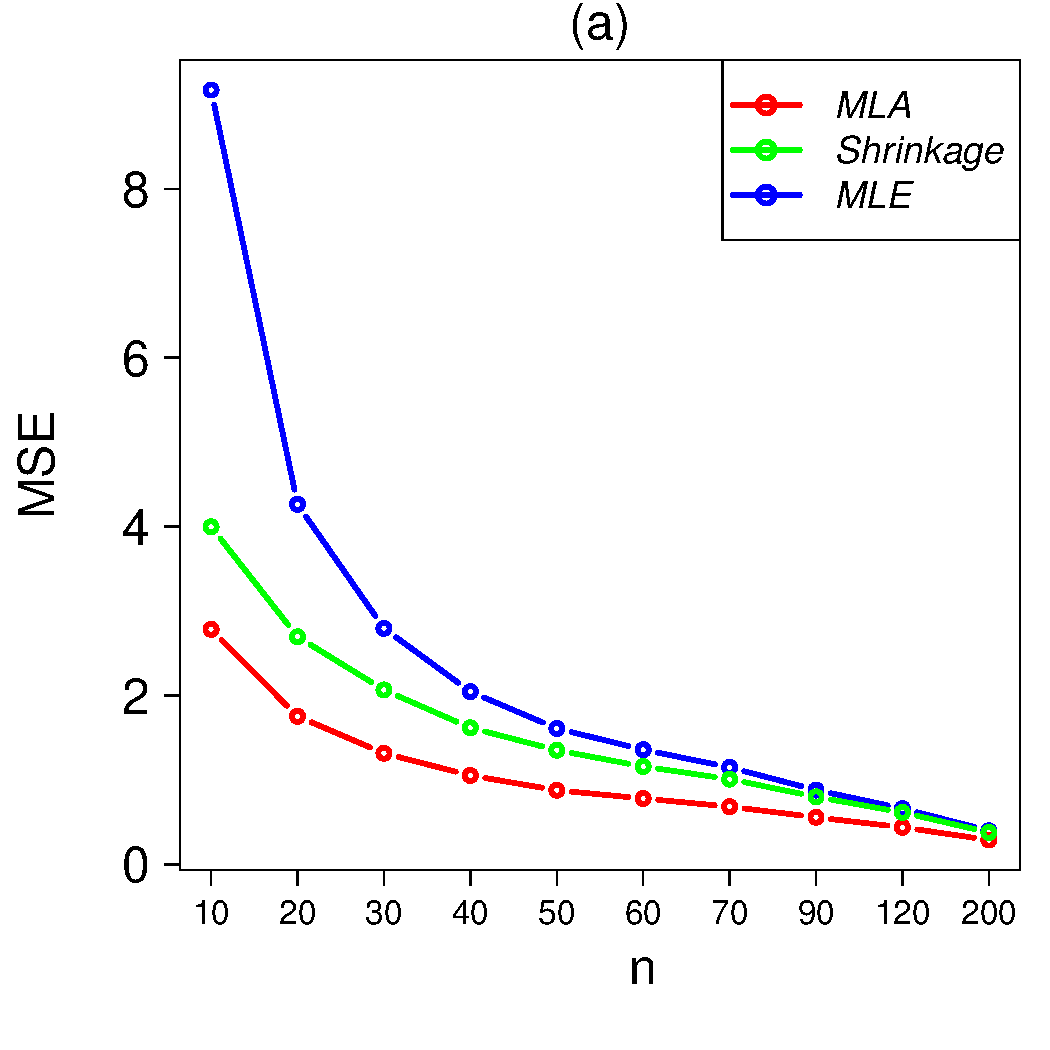
\includegraphics[scale=0.33]{FIG4_4a.pdf}
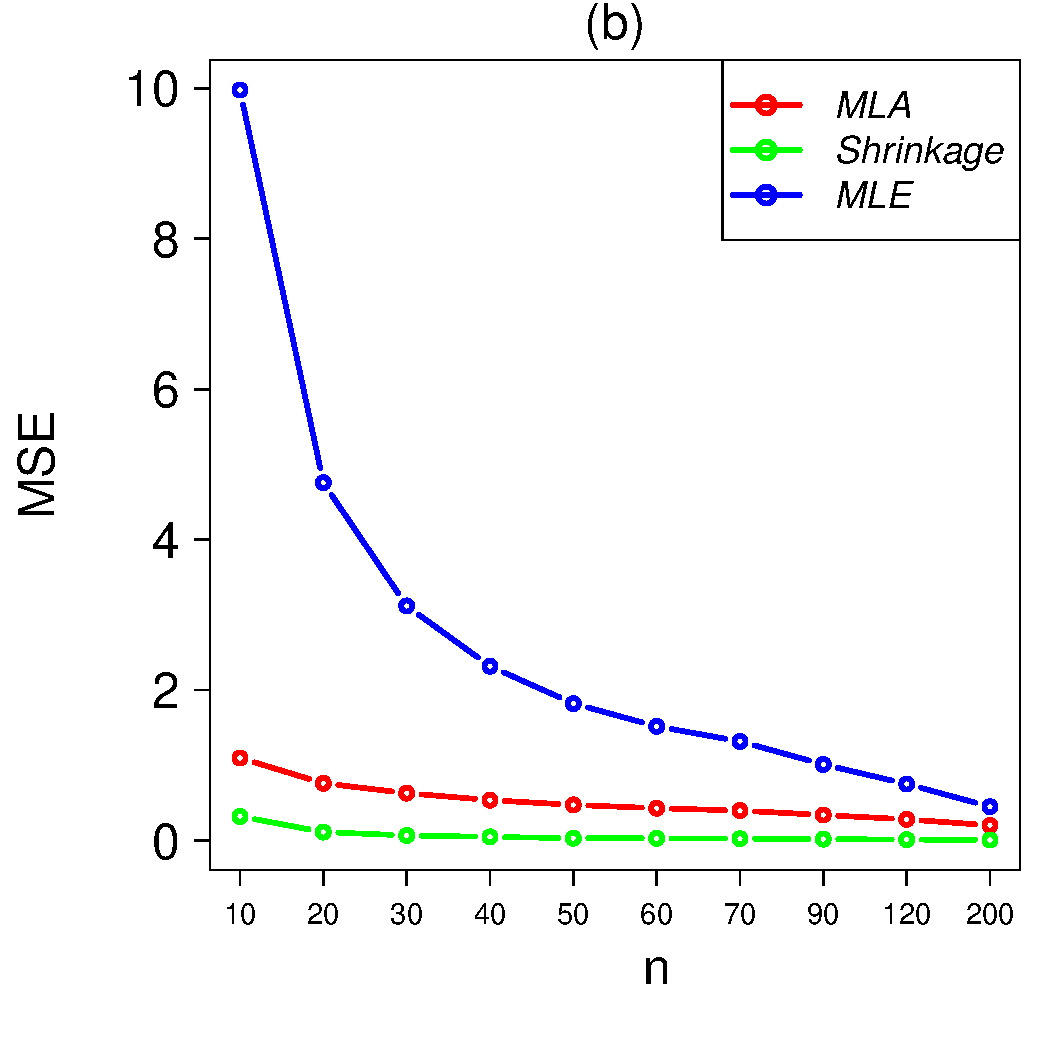
\includegraphics[scale=0.33]{FIG4_4b.pdf}
\end{array}$
\end{center}
\begin{center}$
\begin{array}{ll}
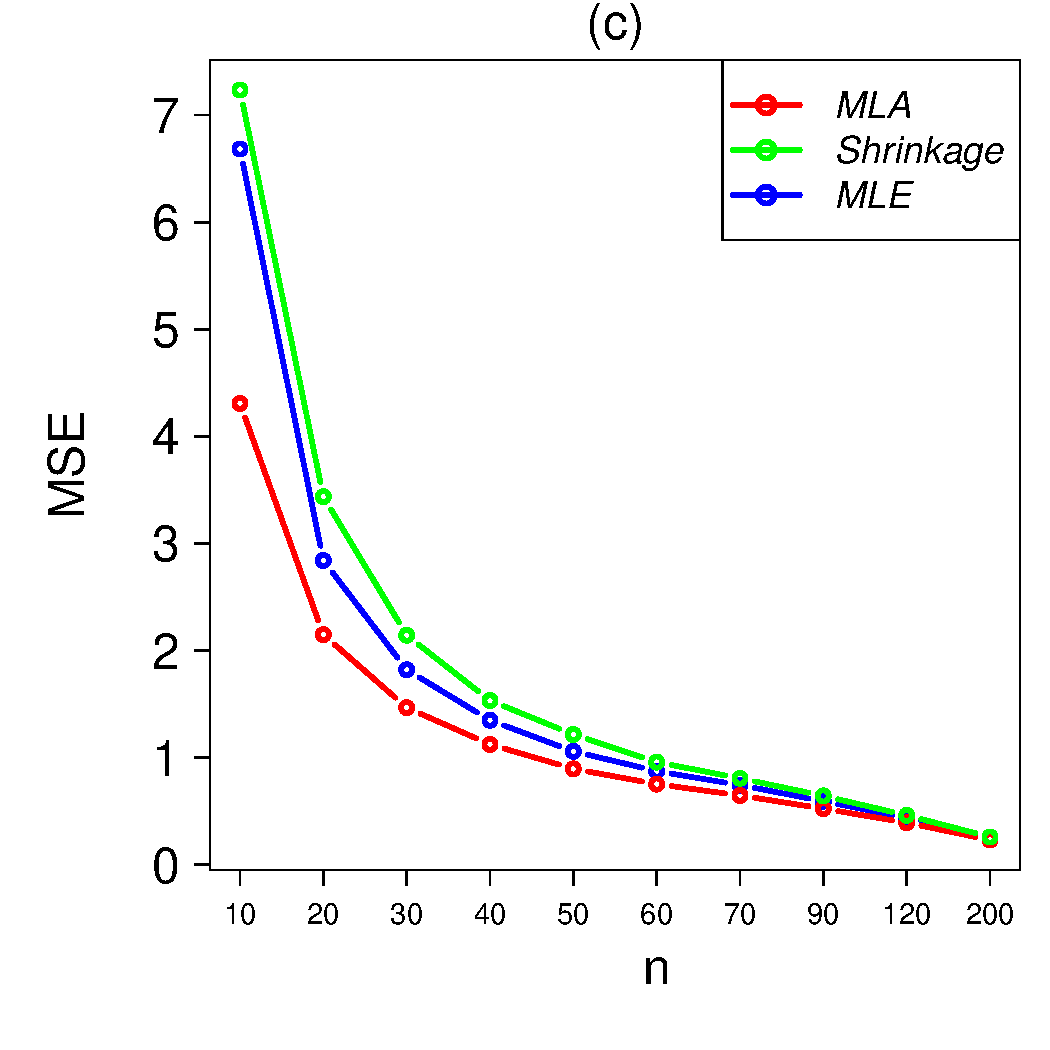
\includegraphics[scale=0.33]{FIG4_4c.pdf}
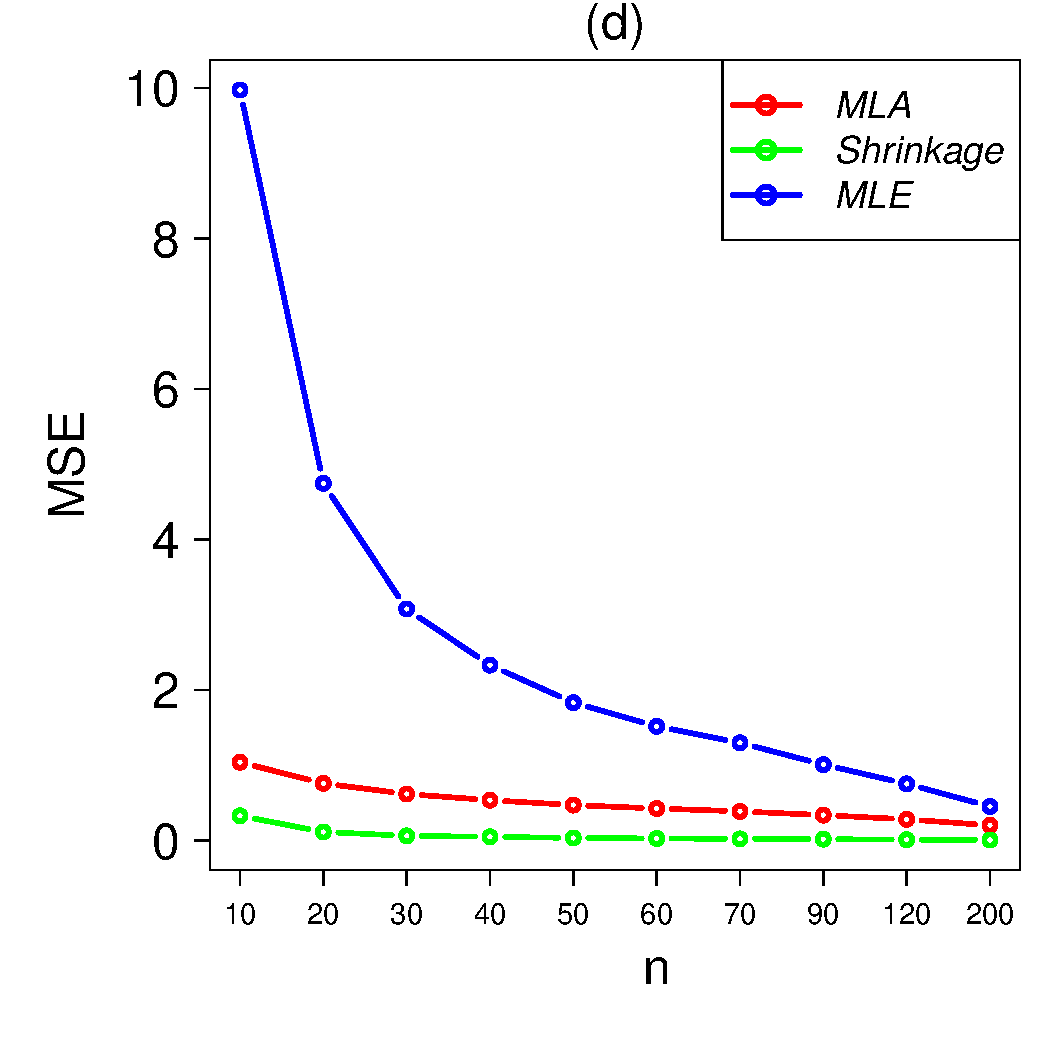
\includegraphics[scale=0.33]{FIG4_4d.pdf}
\end{array}$
\end{center}
\begin{center}$
\begin{array}{r}
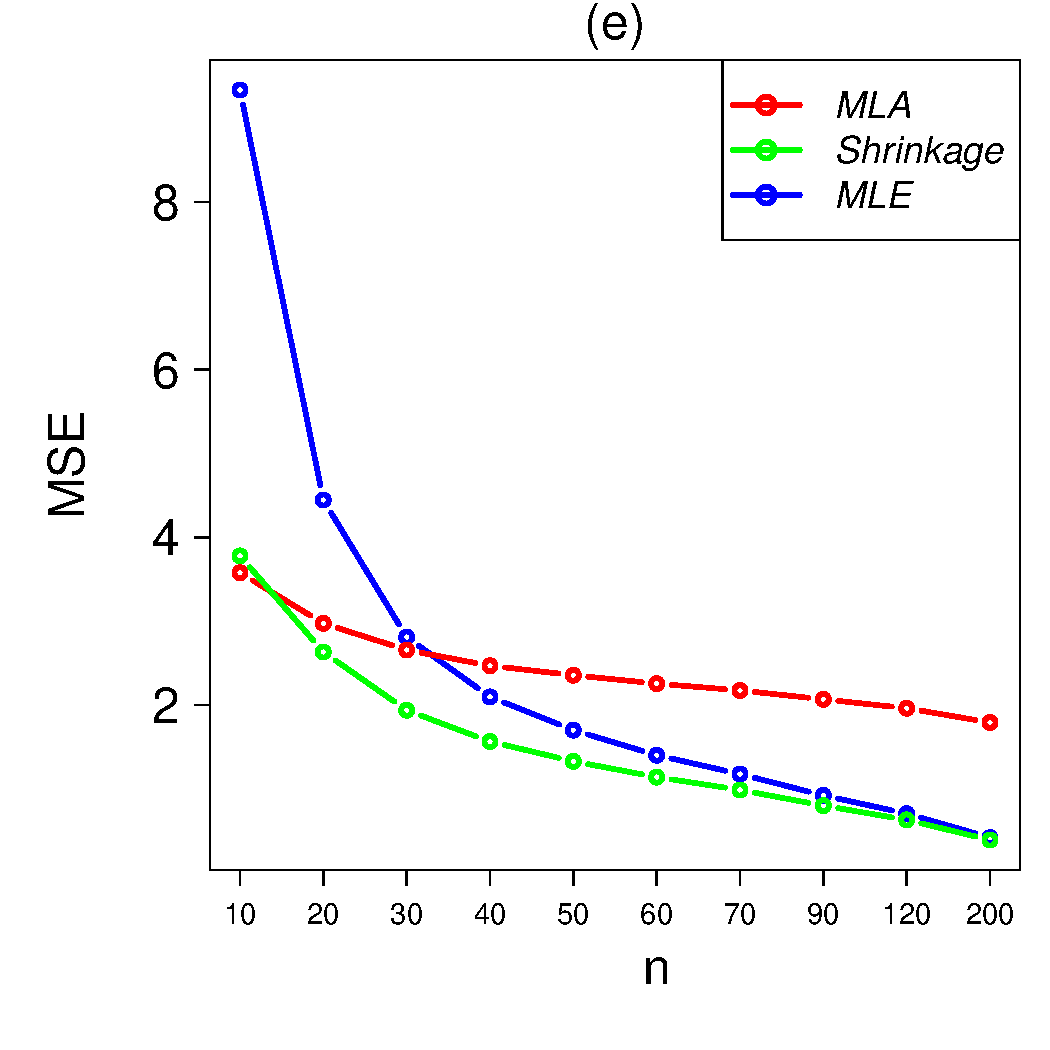
\includegraphics[scale=0.33]{FIG4_4e.pdf}
\end{array}$
\end{center}
\caption{Comparison of MSE averaged over 1000 simulations of the estimated covariance matrices. The data are drawn from multivariate normal distribution with sample size $n=\lbrace10, 20,30,40,50,60,70,90,120,200\rbrace$ and $p=10$ under different choices of covariance matrices (a, b) AR(1) with $t=0.5$ and identity as true covariance matrix for all three methods and AR(1) as a target for the proposed method (c, d) exchangeable with $t=0.5$ and identity as true covariance matrix for all three methods and exchangeable as a target for the proposed method (e) random covariance structure with 30\% off-diagonal entries as non-zero and identity matrix as a target.}
\label{Fig2}
\end{figure}

 
%\begin{figure}[h]
%\centering
%\begin{subfigure}[t]{.4\textwidth}
%\centering
%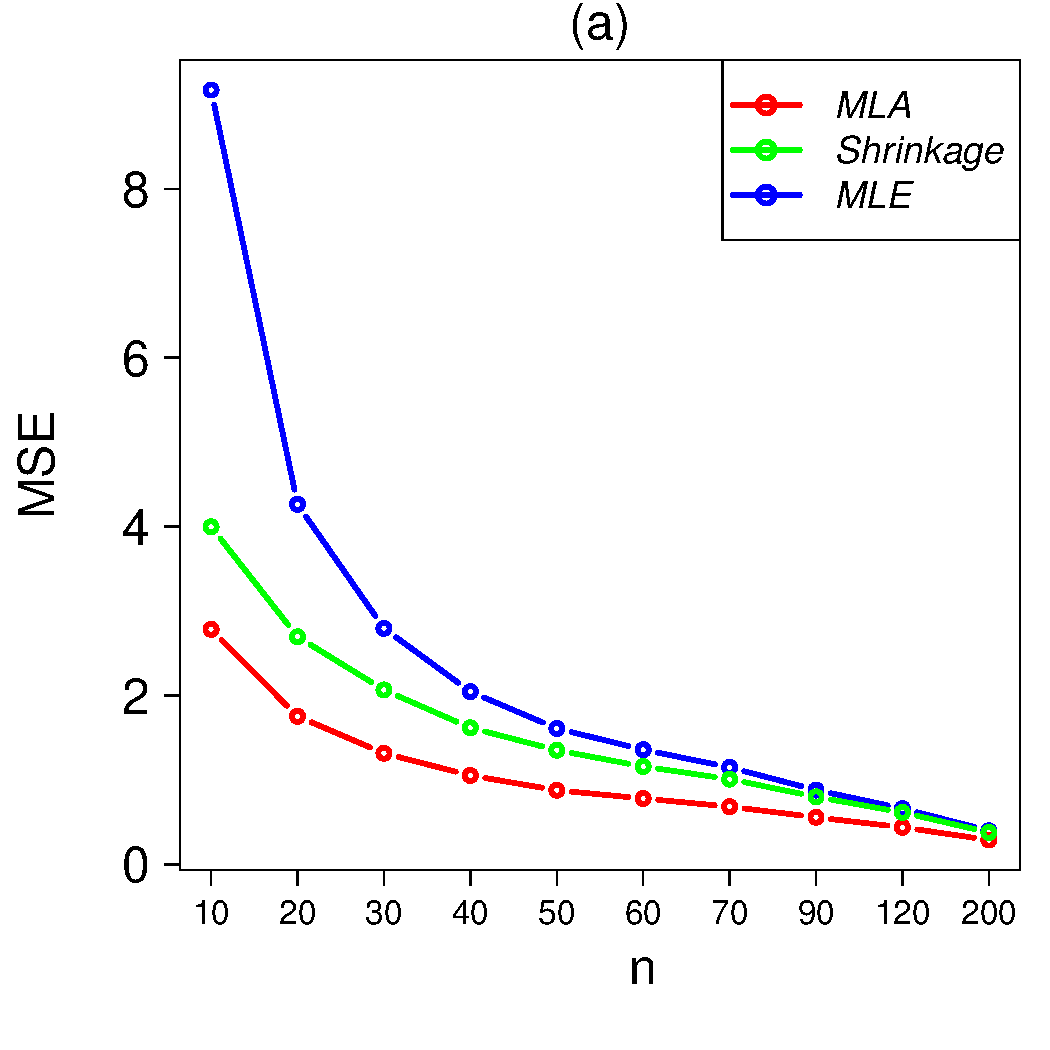
\includegraphics[width=\linewidth]{FIG4_4a.pdf}
%\end{subfigure}
%\begin{subfigure}[t]{.4\textwidth}
%\centering
%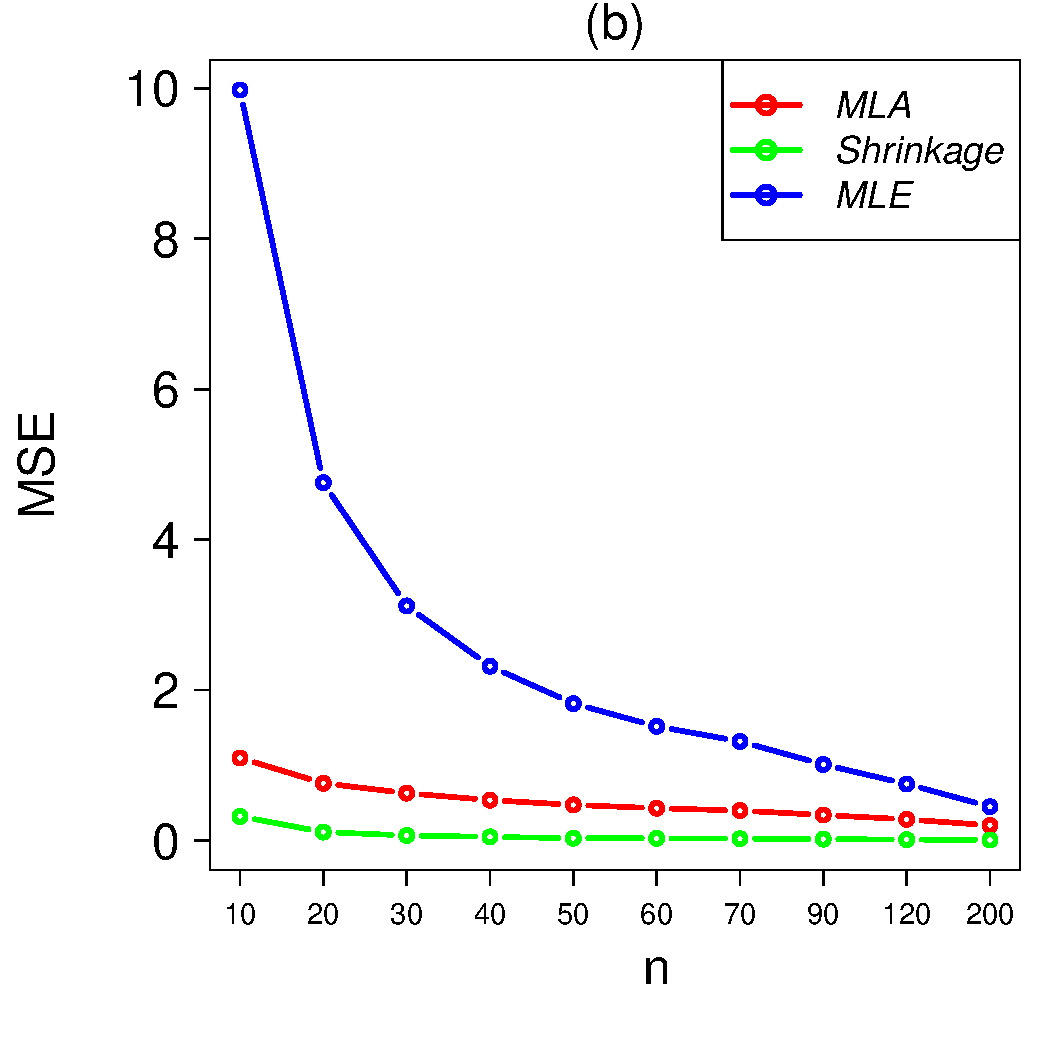
\includegraphics[width=\linewidth]{FIG4_4b.pdf}
%\end{subfigure}
%\medskip
%\begin{subfigure}[t]{.4\textwidth}
%\centering
%\vspace{0pt}
%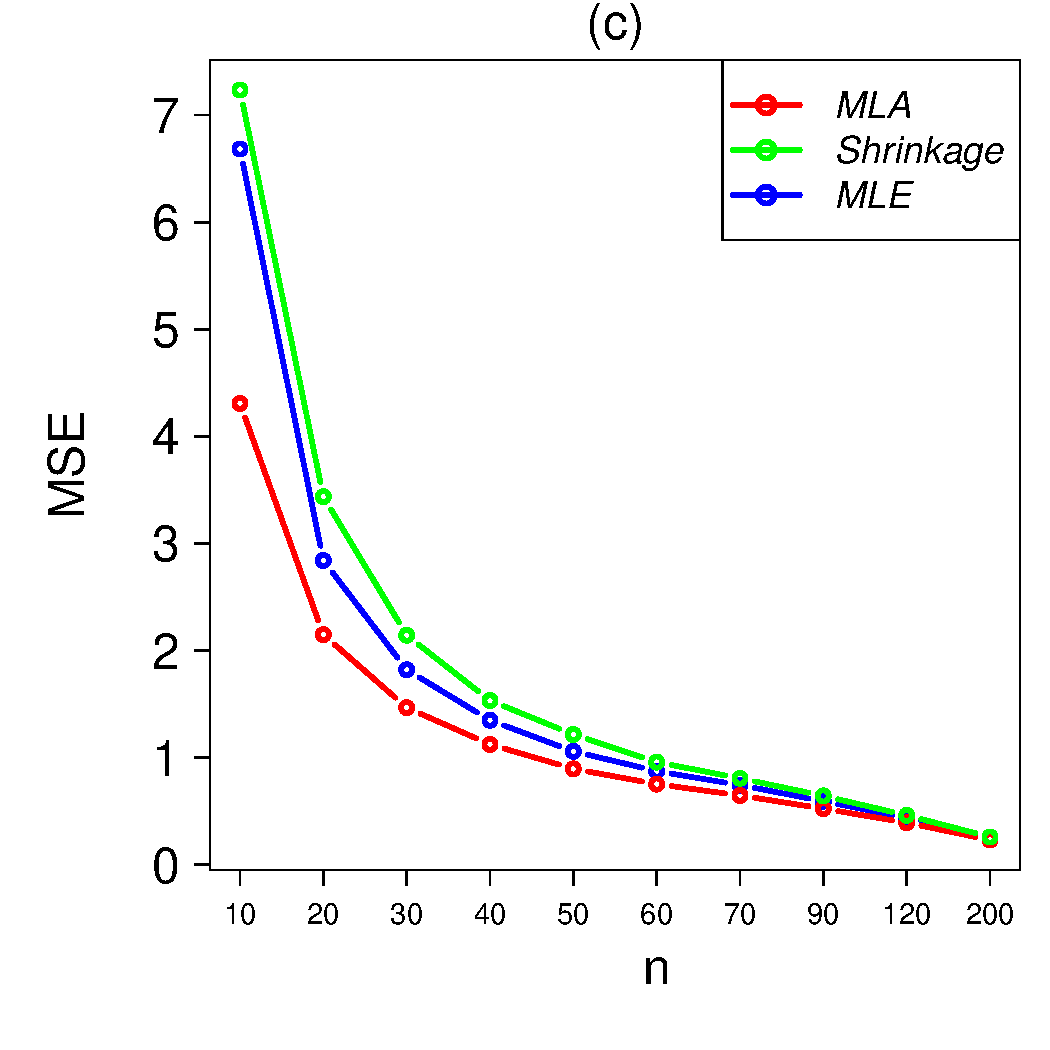
\includegraphics[width=\linewidth]{FIG4_4c.pdf}
%\end{subfigure}
%\begin{subfigure}[t]{.4\textwidth}
%\centering
%\vspace{0pt}
%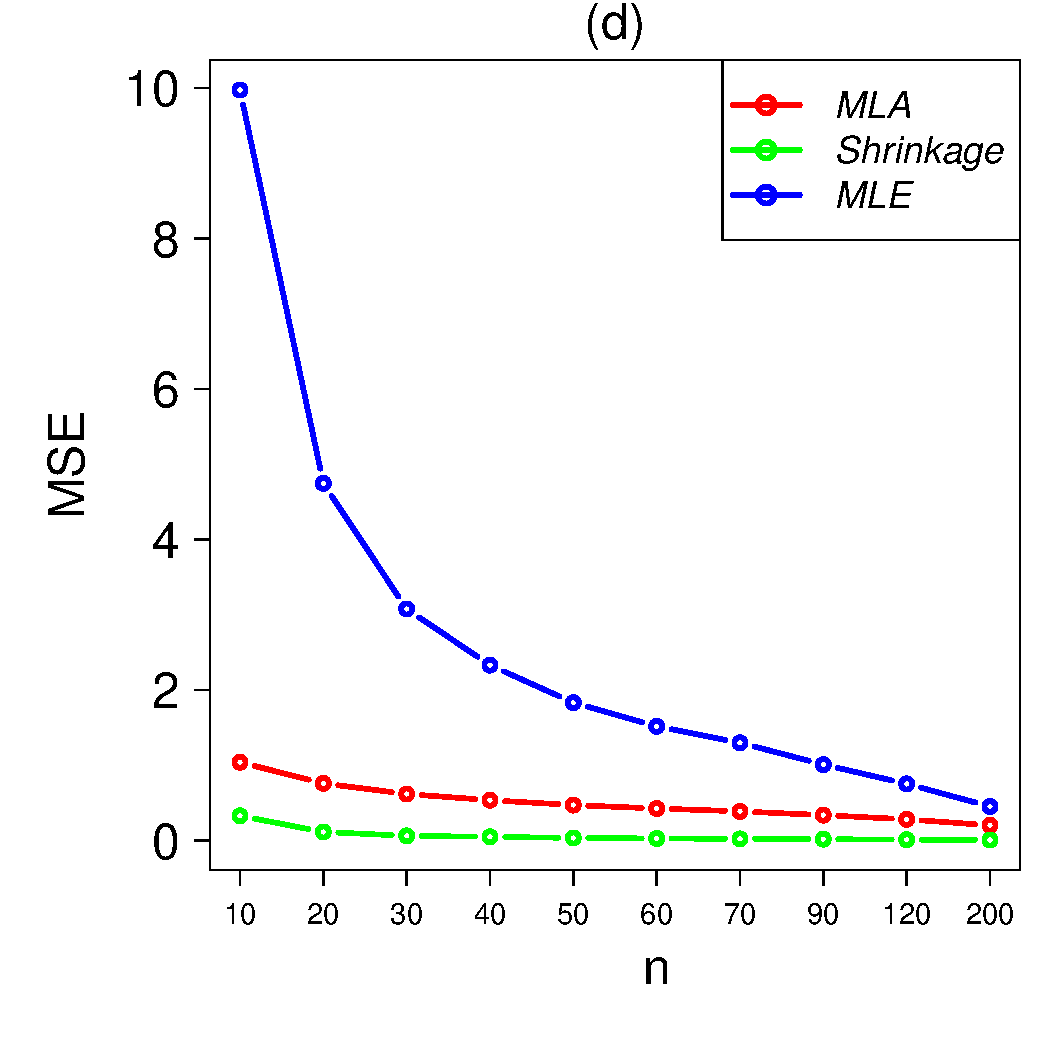
\includegraphics[width=\linewidth]{FIG4_4d.pdf}
%\end{subfigure}
%\begin{subfigure}[t]{.4\textwidth}
%\centering
%\vspace{0pt}
%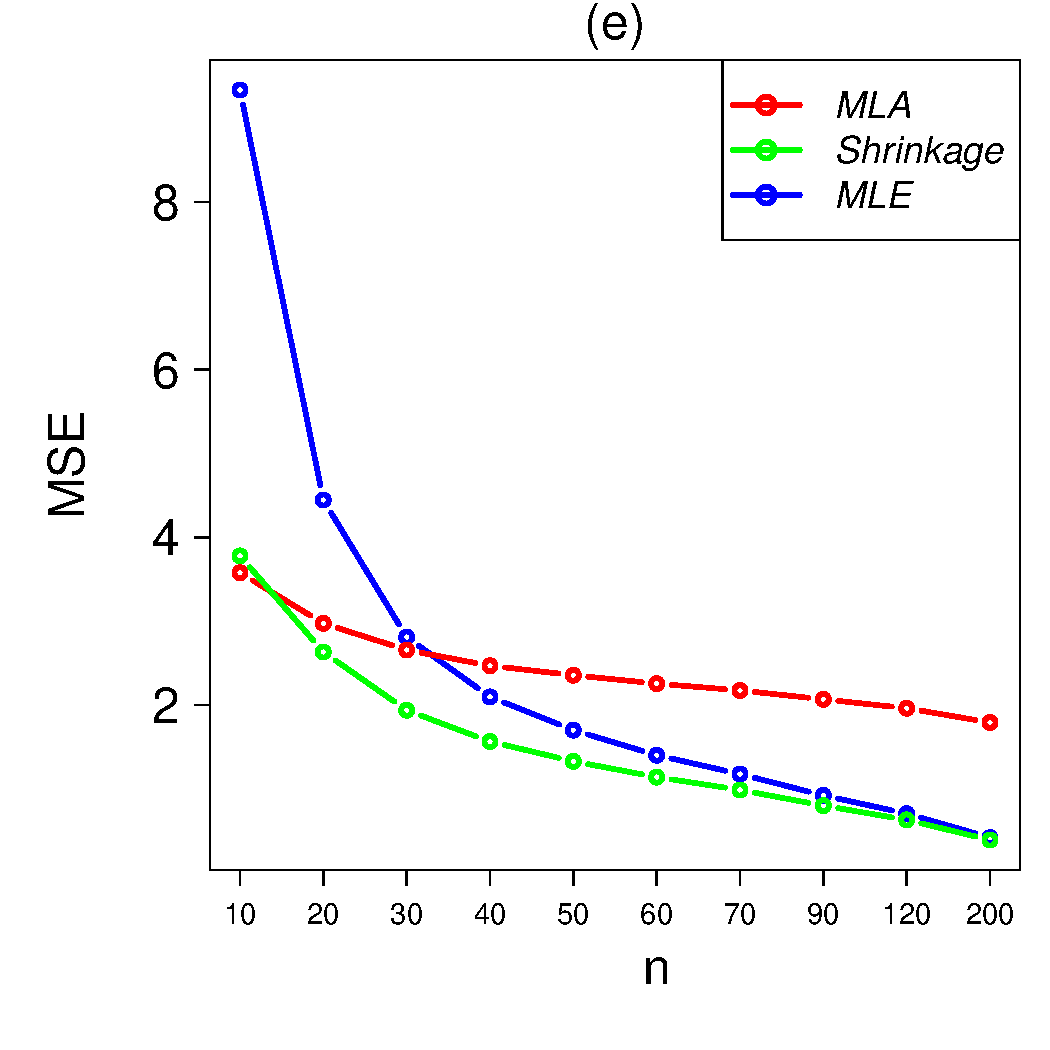
\includegraphics[width=\linewidth]{FIG4_4e.pdf}
%\end{subfigure}
%\caption{Comparison of MSE averaged over 1000 simulations of the estimated covariance matrices. The data are drawn from multivariate normal distribution with sample size $n=\lbrace10, 20,30,40,50,60,70,90,120,200\rbrace$ and $p=10$. Three different structures of the covariance matrices and targets only for the proposed method arranged in Table \ref{Tab1} are used. For random covariance structure we took 30\% off-diagonal entries as being non-zero.}
%\label{Fig2}
%\end{figure}
%, i.e, (a, b) AR(1) covariance structure with targets AR(1) and identity matrix and $t=0.5$, (c, d) exchangeable covariance structure with targets exchangeable and identity matrix and $t=0.5$, (c)
%In third experiment, we plot the eigenvalues of the estimated covariance matrices of proposed method, shrinkage method of \cite{schafer2005shrinkage}, maximum likelihood method and eigenvalues of the true covariance matrix. We set $n=30$ and $p=50$ and use the same covariance structures to simulate the data from multivariate normal distribution and targets for different covariance structures as was used in the above two experiments, the only difference in this case is that for exchangeable covariance structure we consider $t=0.3$

In the previous case, we demonstrated the estimation error in eigenvalues. Here we visually compare the estimated eigenvalues with the true eigenvalue. Although we have conducted a range of simulation experiments, we show the results for $n=30$ and $p=50$ and generate the data from multivariate normal distribution using all three covariance structures mentioned above. For AR(1) and exchangeable covariance structures we consider $t=0.5$ and $t=0.3$, respectively. For random covariance structure we take 30\% of the off-diagonal elements as being non-zero. Furthermore, when the true covariance matrices are AR(1) and exchangeable we shrink the sample covariance matrix, respectively, towards AR(1) and exchangeable targets, which are correct targets for AR(1) and exchangeable covariance structures. For identity as a true covariance matrix we also use both AR(1) and exchangeable targets to shrink the sample covariance matrix towards them, which are incorrect targets. However, for random covariance structure we use only identity matrix as a target. We then estimate the covariance matrix using the proposed and shrinkage methods and calculate the eigenvalues of the two competing estimators along with the eigenvalues of sample covariance and true covariance matrix (gold standard). These eigenvalues are presented in Figure \ref{Fig3} averaged over 1000 simulations for all three the estimated covariance matrices. 
\section*{Results:}
From Figure \ref{Fig3} it can be seen that the sample eigenvalues are highly inaccurate that is the large eigenvalues overestimated and the small eigenvalues are under estimated. The proposed method and shrinkage method of \cite{schafer2005shrinkage} overcome this problem. But the eigenvalues of the proposed method recover the true eigenvalues more accurately compare to the shrinkage method of \cite{schafer2005shrinkage} if the target is correctly specified in case of AR(1) and exchangeable covariance structures. When the target is incorrectly specified in that case the eigenvalues estimated using shrinkage method are slightly closer to the true eigenvalues as compare to the proposed method. For random covariance structure the eigenvalues obtained from the proposed estimator are more accurate. 

\begin{figure}[H]
\begin{center}$
\begin{array}{ll}
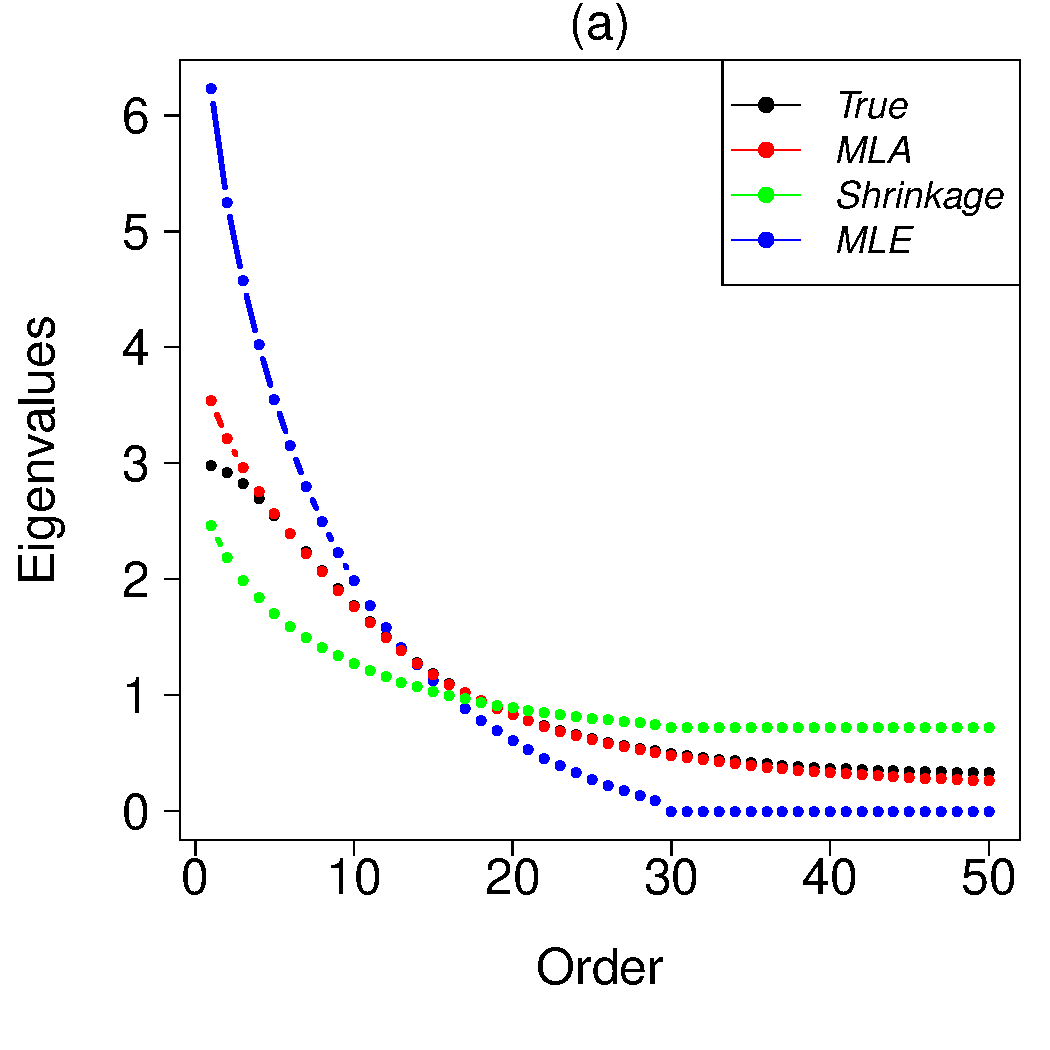
\includegraphics[scale=0.33]{FIG4_3a.pdf}
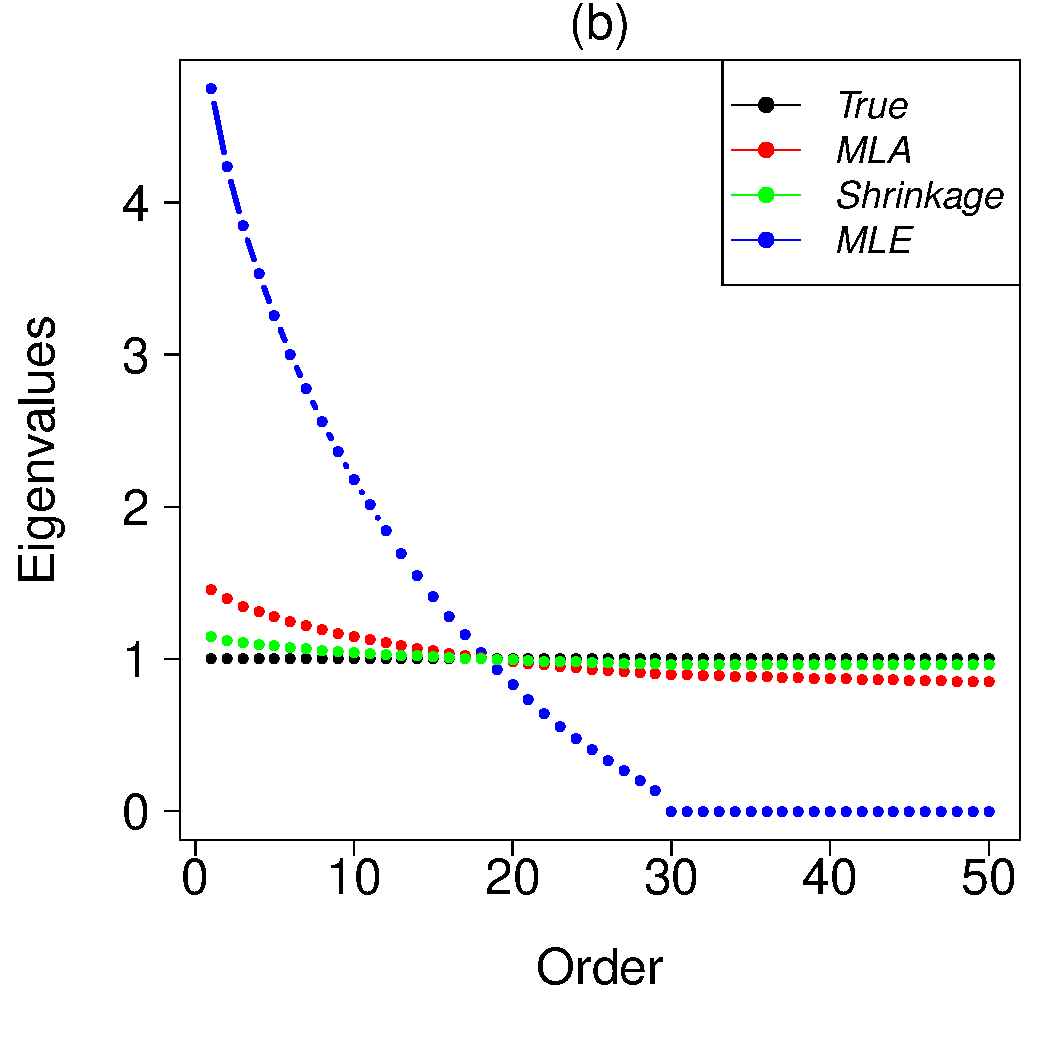
\includegraphics[scale=0.33]{FIG4_3b.pdf}
\end{array}$
\end{center}
\begin{center}$
\begin{array}{ll}
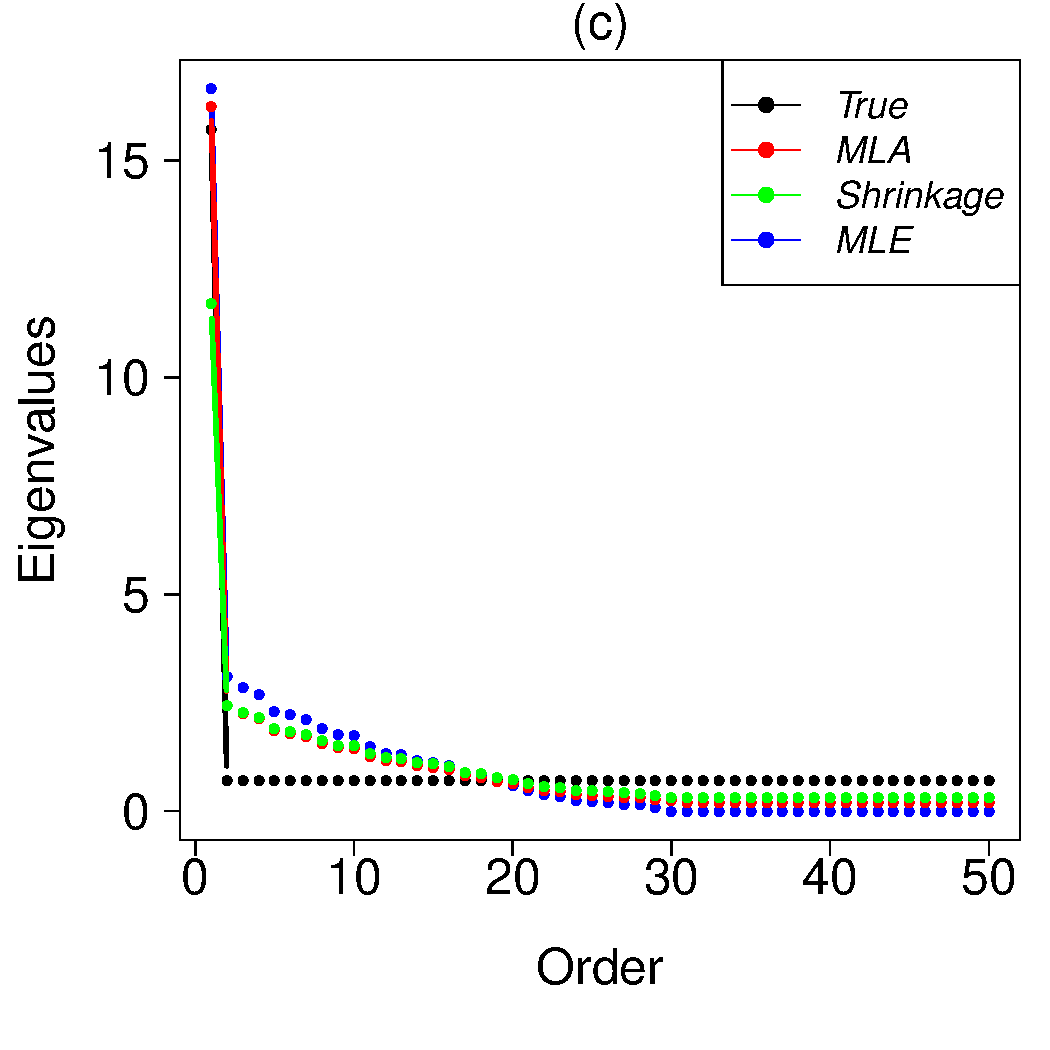
\includegraphics[scale=0.33]{FIG4_3c.pdf}
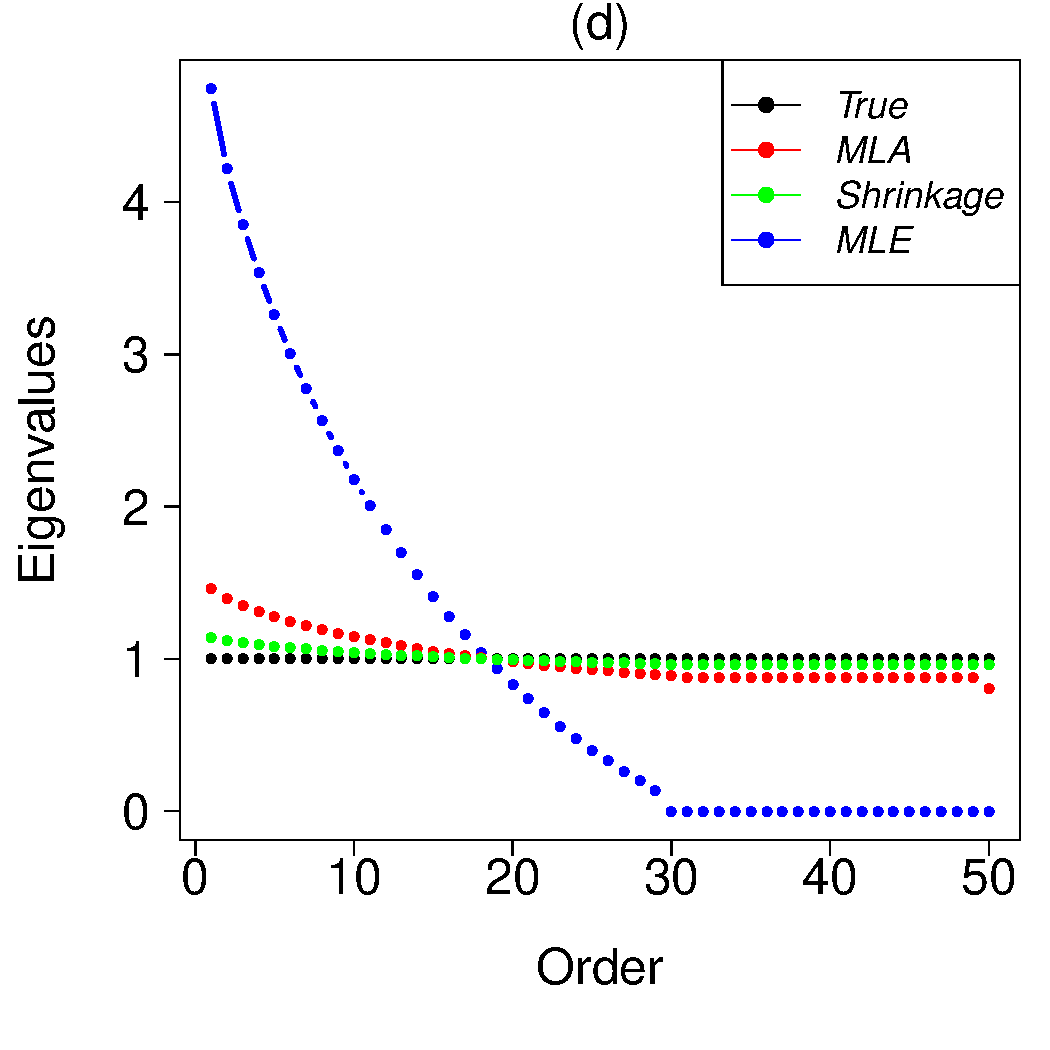
\includegraphics[scale=0.33]{FIG4_3d.pdf}
\end{array}$
\end{center}
\begin{center}$
\begin{array}{r}
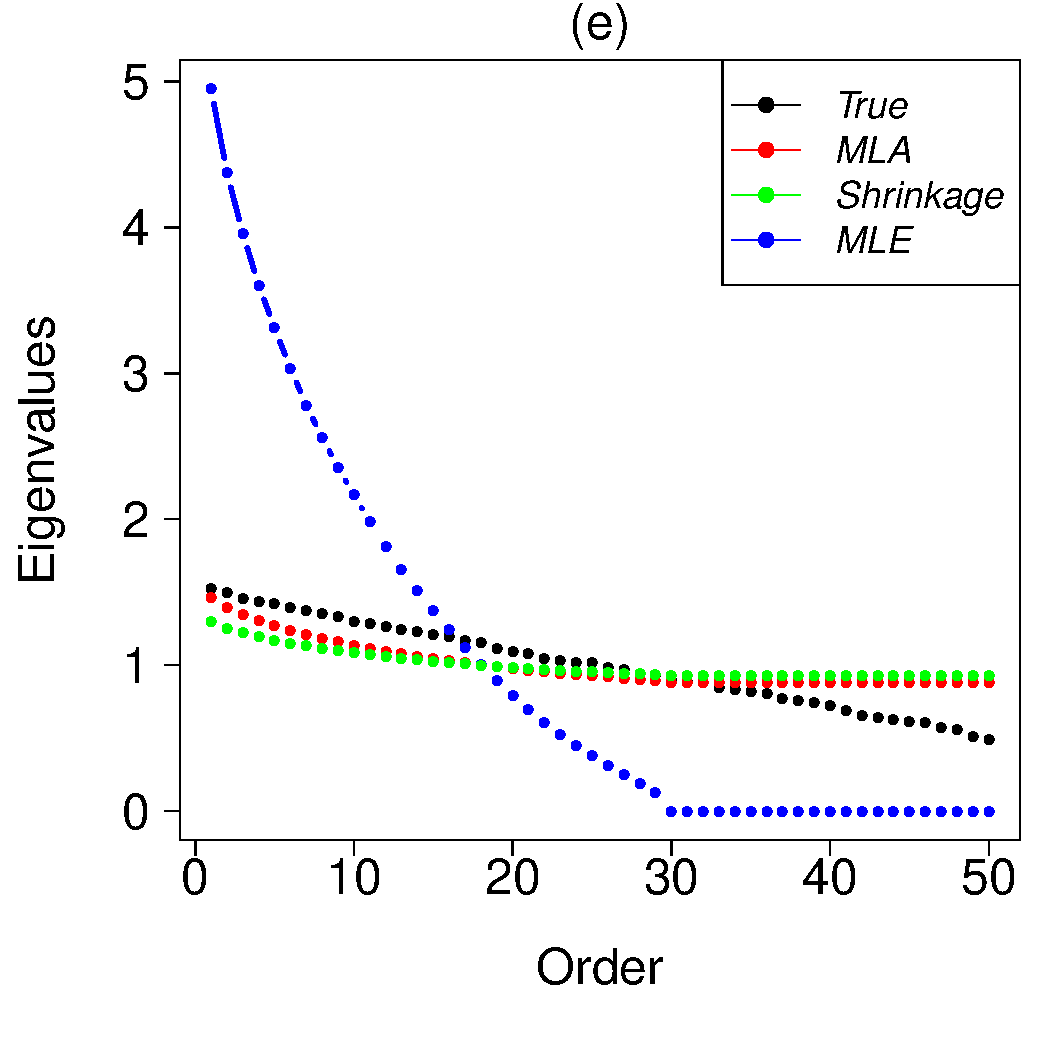
\includegraphics[scale=0.33]{FIG4_3e.pdf}
\end{array}$
\end{center}
\caption{Comparison of estimated and true eigenvalues with $n=30$ and $p=50$ averaged over 1000 simulation. The data are drawn from multivariate normal distribution under different choices of covariance matrices (a, b) AR(1) with $t=0.5$ and identity as true covariance matrix for all three methods and AR(1) as a target for the proposed method (c, d) exchangeable with $t=0.3$ and identity as true covariance matrix for all three methods and exchangeable as a target for the proposed method (e) random covariance structure with 30\% off-diagonal entries as non-zero and identity matrix as a target.}
\label{Fig3}
\end{figure}


%\begin{figure}[h]
%\centering
%\begin{subfigure}[t]{.4\textwidth}
%\centering
%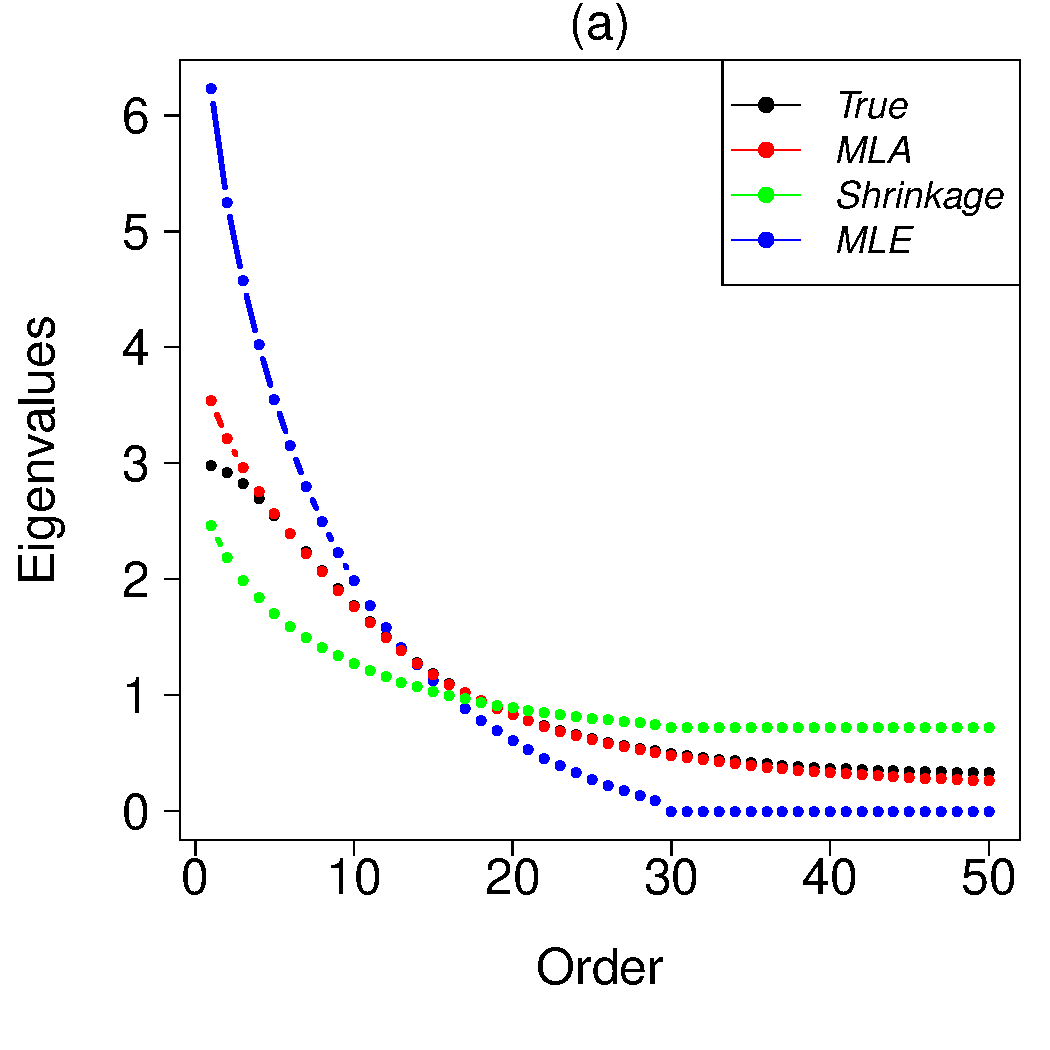
\includegraphics[width=\linewidth]{FIG4_3a.pdf}
%\end{subfigure}
%\begin{subfigure}[t]{.4\textwidth}
%\centering
%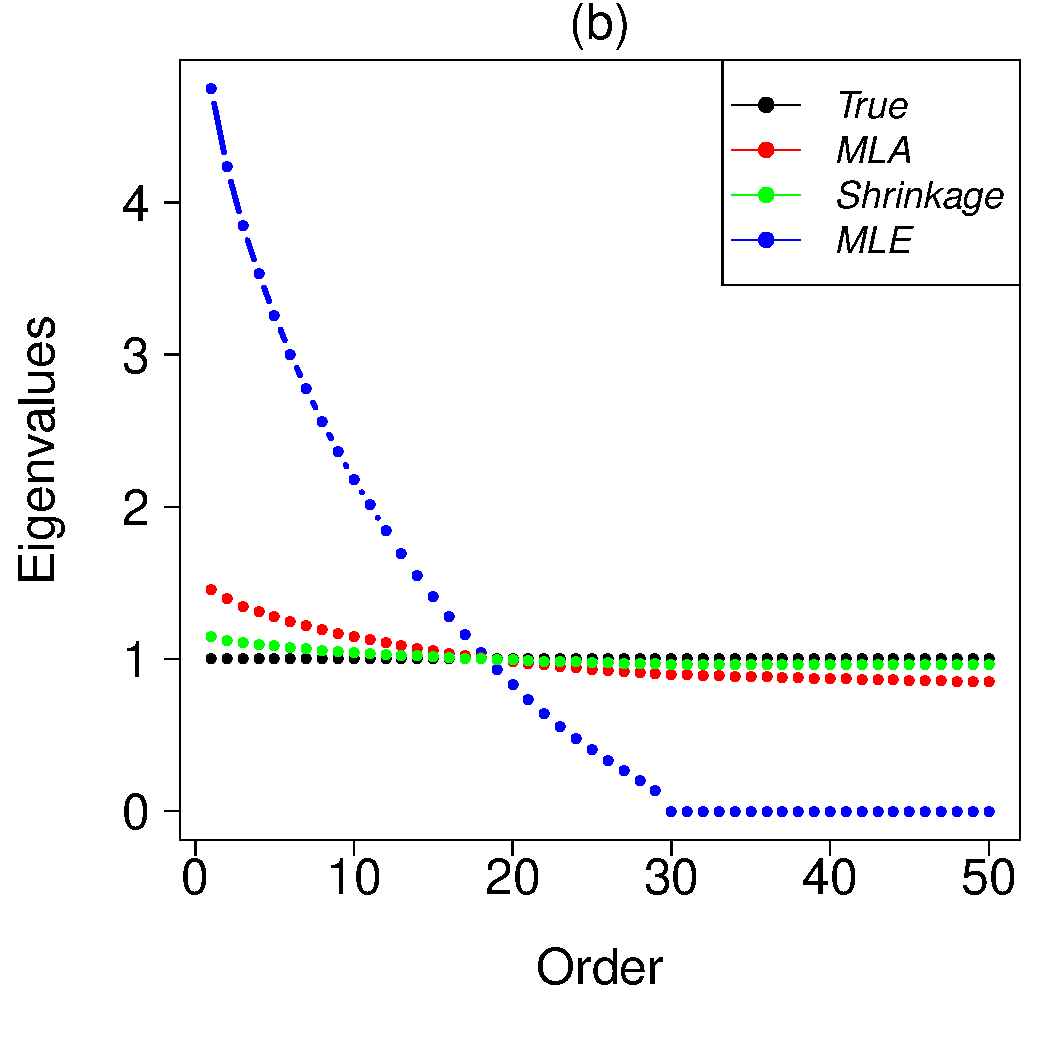
\includegraphics[width=\linewidth]{FIG4_3b.pdf}
%\end{subfigure}
%\medskip
%\begin{subfigure}[t]{.4\textwidth}
%\centering
%\vspace{0pt}
%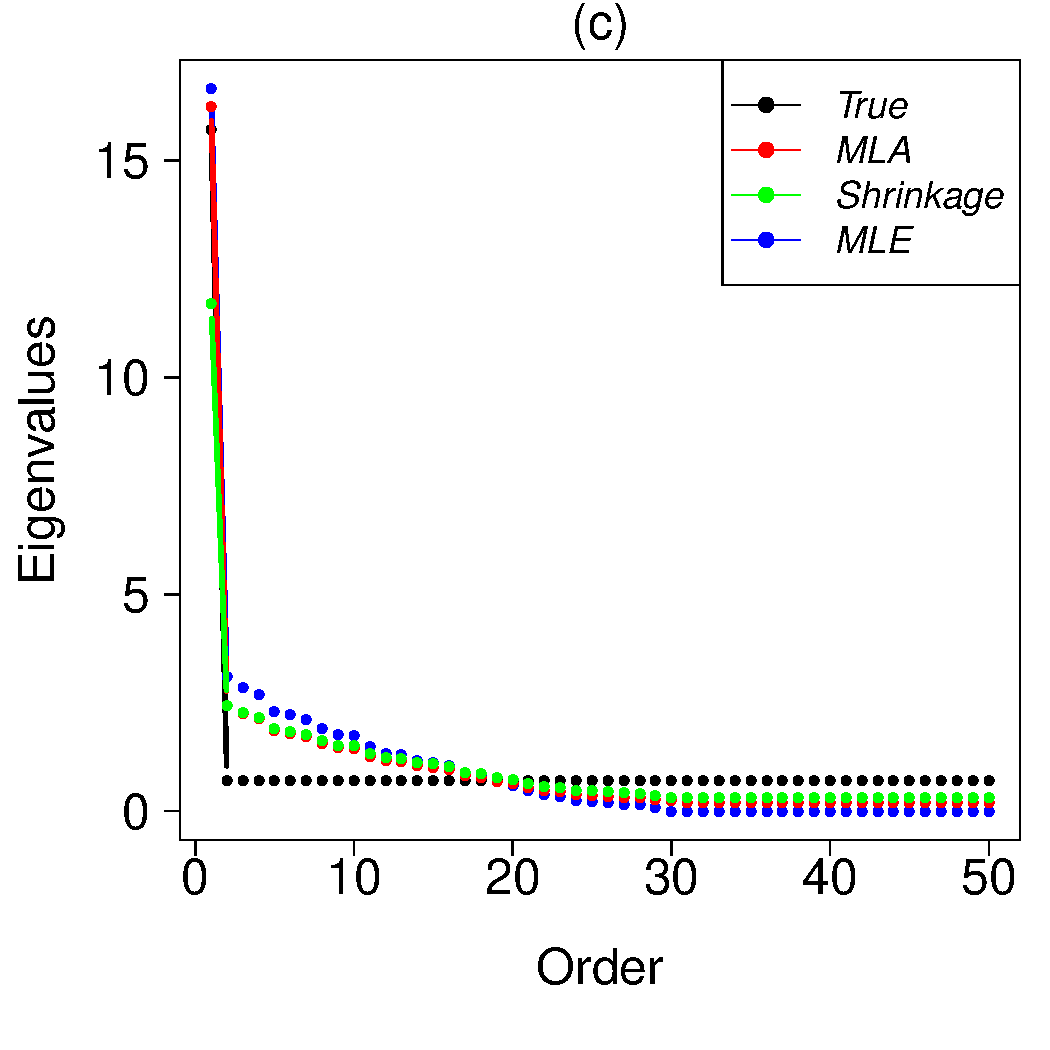
\includegraphics[width=\linewidth]{FIG4_3c.pdf}
%\end{subfigure}
%\begin{subfigure}[t]{.4\textwidth}
%\centering
%\vspace{0pt}
%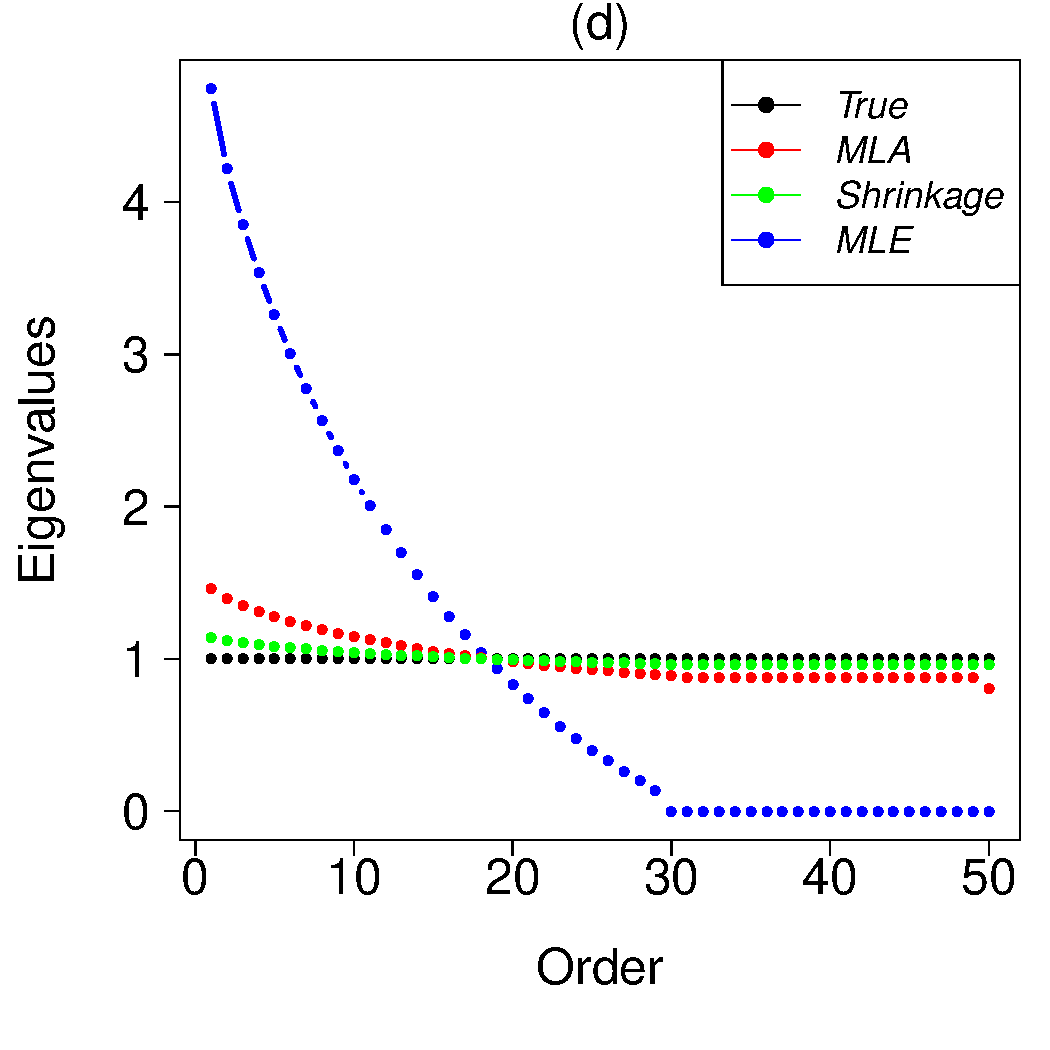
\includegraphics[width=\linewidth]{FIG4_3d.pdf}
%\end{subfigure}
%\begin{subfigure}[t]{.4\textwidth}
%\centering
%\vspace{0pt}
%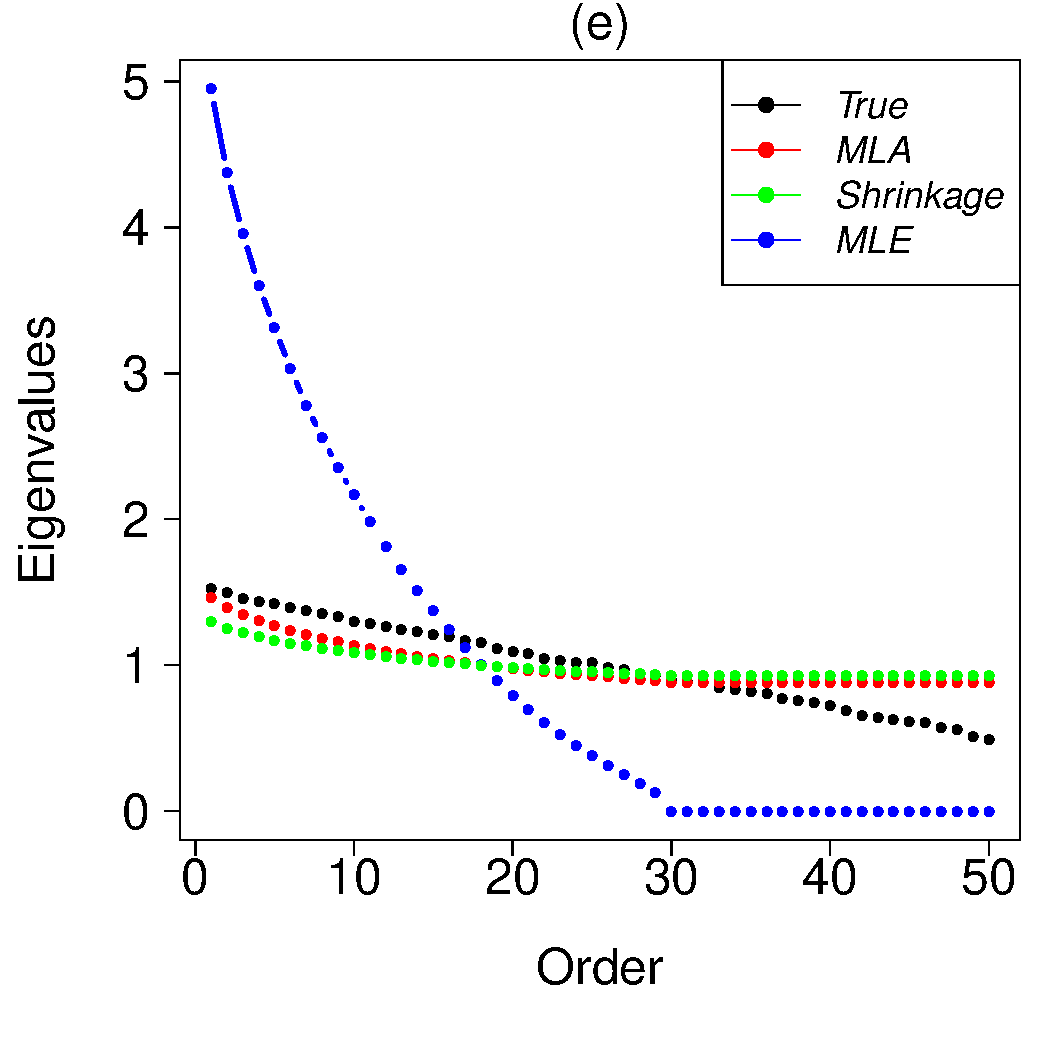
\includegraphics[width=\linewidth]{FIG4_3e.pdf}
%\end{subfigure}
%\caption{Comparison of the estimated and true eigenvalues with $n=30$ and $p=50$ averaged over 1000 simulation. The data are drawn from multivariate normal distribution under different covariance structures arranged in Table \ref{Tab1} with different targets for the proposed method. For random covariance structure we took 30\% off-diagonal entries as being non-zero.}
%\label{Fig3}
%\end{figure}
 
\chapter{Conclusion}
\lhead{Chapter 5. \emph{Conclusion}}


In high-dimensional data where sample size is smaller than the number of variables, the sample estimator of the covariance matrix is not invertible and contains a large amount of estimation error. In these situations the classical multivariate techniques, which rely on the covariance matrix or its inverse, either fails to work or becomes unreliable (when $n$ is larger but comparable to $p$). To overcome this problem various methods have been proposed in the literature to improve upon the sample estimator such as Moore-Penrose generalized inverse and other shrinkage estimation methods. 

In this study a new regularized method of the covariance matrix is developed, which is also like shrinkage estimation is the linear convex combination of the sample covariance matrix and a target matrix. This new regularized estimator depends on the penalty parameter whose value need to be chosen in the appropriate range of values. The value of the penalty parameter is achieved by maximizing the log-likelihood function of the multivariate normal distribution. The proposed estimator is not only invertible but also well-conditioned. Furthermore, two new more informative targets have been used to shrink the sample covariance matrix towards them. These targets are the AR(1) and exchangeable covariance structures, which depends on the correlation parameter and need to be estimated in the appropriate range of values. To choose an appropriate value of the correlation parameter maximum log-likelihood function of the multivariate normal distribution is used. 

The behaviour of the proposed method compare to the shrinkage method is explored through large simulations. The simulation experiments show that the proposed estimator perform better than the shrinkage estimator whenever the target is correctly specified in case of AR(1) and exchangeable covariance structures. However, its performance becomes slightly weaker than the shrinkage estimator when the target is incorrectly specified as AR(1) or exchangeable while the true covariance matrix is identity matrix. In case of random covariance structure our proposed estimator perform better than the shrinkage estimator.

It is worth noticing that the proposed estimator is also analytically much simpler and computationally inexpensive procedure compare to the shrinkage method.
 
 

%----------------------------------------------------------------------------------------
%	THESIS CONTENT - APPENDICES
%----------------------------------------------------------------------------------------

\addtocontents{toc}{\vspace{2em}} % Add a gap in the Contents, for aesthetics

\appendix % Cue to tell LaTeX that the following 'chapters' are Appendices

% Include the appendices of the thesis as separate files from the Appendices folder
% Uncomment the lines as you write the Appendices

% Appendix A

\chapter{R codes for Figures} % Main appendix title

\label{AppendixA} % For referencing this appendix elsewhere, use \ref{AppendixA}

\lhead{Appendix A. \emph{R codes}} % This is for the header on each page - perhaps a shortened title

\lstset{ language=R, basicstyle=\ssmall,  morekeywords={TRUE,FALSE}, keywordstyle=\color{blue}\itshape, commentstyle=\color{DarkGreen} ,stringstyle=\color{DarkGreen}, numbers=left, numberstyle=\ttfamily\color{gray}\footnotesize, stepnumber=1, numbersep=5pt, backgroundcolor=\color{lightgray}, showspaces=false, showstringspaces=false, showtabs=false, frame=single, tabsize=2, captionpos=b, breaklines=true, breakatwhitespace=false, title=\lstname, escapeinside={}, otherkeywords={0,1,2,3,4,5,6,7,8,9}}
%\lstset{% general command to set parameter(s)
%basicstyle=\small, % print whole listing small
%keywordstyle=\color{red}\itshape,
% underlined bold black keywords
%commentstyle=\color{blue}, % white comments
%stringstyle=\ttfamily, % typewriter type for strings
%showstringspaces=false,
%numbers=left, numberstyle=\tiny, stepnumber=1, numbersep=5pt, %
%frame=shadowbox,
%rulesepcolor=\color{black},
%,columns=fullflexible
%}
Functions to be used in some Figures R codes. 
\begin{lstlisting}
t.ar1 <-  function(x) { # The function that estimate "t" in case of AR(1)
  n <- nrow(x)          # covariance structure given in equation 3.19. 
  p <- ncol(x)          # We will mention it in a comment wherever it is
  cor.psi <- cor(x)     # required
  sum <- 0
  for(t in 2:p){
    sum <- sum + cor.psi[t,t-1]
  }
  hat.t <- sum/(p-1)
}

t.exch <-  function(x) { # The function that estimate "t" in case of
  n <- nrow(x)           # exchangeable covariance structure given in
  p <- ncol(x)           # equation 3.13. We will mention it in a 
  cc <- cor(x)           # comment wherever it is required
  sum <- 0
  for(i in 1:(p-1)){
    for(j in (i+1):p){
      sum <- sum + cc[i,j]
    }
  }
  hat.t <- 2*sum/(p*(p-1))
}

un.str.cov <- function(n.var, prop.non.zero, const){ # The function to compute the
  AA <- matrix(0, n.var, n.var)      # random covariance structure of Schafer &         
  SS <- matrix(0, n.var, n.var)      # Strimmmer (2004) We will mention it in a
                                     # comment wherever it is required  
  AA[upper.tri(AA)] <- c(rbinom(n.var*(n.var-1)/2,1,prop.non.zero)) # proportion of non-zero elements
  
  BB <- AA + t(AA)
  for (i in 1:(n.var-1)){
    for (j in (i+1):n.var){
      if (AA[i,j]==1){
        SS[i,j] <- runif(1,-1,1) # Replace 1s with random values from the uniform distribution
      }
    }
  }
  
  SS <- SS + t(SS)
  ABS.SS <- abs(SS)
  ColSum <- apply(ABS.SS, 2, sum)
  
  for (i in 1:n.var){
    SS[i,i] <- ColSum[i] + const # fill diagonal entries with column sum plus small positive constant
  }
  
  cov2cor(SS)
}
\end{lstlisting}

Figure \ref{Fig1}.
\begin{lstlisting}
library(MASS) # Library "Modern Applied Statistics with S" abbreviated as MASS must be installed before running these R codes and will be used for all Figures R codes.  
 
# Different sample sizes "n" and fixed "p"
n <- c(25,50,100,1000)
p <- 50

# Null matrix needed for results inside for loop to be used for further analysis
mat <- matrix(NA, nrow=length(n), ncol=p)

# True covariance and its eigenvalues
sigma <- diag(1, nrow = p, ncol = p)
e.tre <- eigen(sigma)$values

# Calculating sample covariance matrix eigenvalues for different samples "n"
for(i in 1:length(n)){
  # Repeat the results 1000 times. We will repeat the results for all Figures in R codes. 
  res <- replicate(1000, {
  # Generating "n * p" X matrix from multivariate normal distribution 
  x <- mvrnorm(n=n[i], mu=rep(0,p), Sigma=sigma)
  # Sample covarince matrix and its eigenvalues
  S <- cov(x)
  S.eigenvalues <- eigen(S)$values
  })
  # Averaging eigenvalues repeated 1000 times
  mat[i,] <- apply(res,1,mean)
}
# y limit for plot
yl <- max(rbind(mat,e.tre))

pdf(file = "screeplot.pdf") 
# plotting true and sample eigenvalues
plot(e.tre,type="b",lwd=3,pch=16, ylim = c(0,yl), xlab="Order", ylab = "Eigenvalues")
points(mat[1,], type="b", lwd=3,pch=16 ,col="red")
points(mat[2,], type="b", lwd=3,pch=16, col="blue")
points(mat[3,], type="b", lwd=3, pch=16,col="5")
points(mat[4,], type="b", lwd=3, pch=16,col="green")

legend("topright",inset = 0.03, legend = c("True","n= 25","n= 50","n= 100","n= 1000"),cex = 1,box.lwd = 2,box.lty = 2,text.font = 4, bg="gray",col = c("black","red","blue","5","green"), lty = 1,  pch = 16)

dev.off()
\end{lstlisting}

Figure (3.1)a
\begin{lstlisting}
library(MASS)

# Various "n" and "p"
n <- c(10, 30, 300)
p <- c(10, 30, 100)

# Null matrix (gamma matrix) needed for gamma values inside for loops to be used for futher analysis
gamma <- matrix(NA, length(n), length(p))
res<- replicate(1000,{
  for(i in 1:length(p)){
    for(j in 1:length(n)){
      # Identity matrix as a true covariance matrix
      sigma <- diag(p[i])
      x <- mvrnorm(n=n[j], mu= rep(0,p[i]), Sigma=sigma)
      
      # Calculate gamma values and store them in null matrix
      gamma[i,j] <- 1/(1+sum(abs(cor(x) - diag(p[i])))/(p[i]))
    }
  }
  gamma
})

# Make the resulting gamma matrix as a vector repeated 1000 times 
vec <- as.vector(res)
# Boxes positions in the boxplot
arr <- as.vector(array(c(1,4,7,2,5,8,3,6,9),dim = c(3,3,1000)))

pdf(file="boxId.pdf")
# Margin
par(mar=c(7,5,1.5,1))
boxplot(vec~arr, outline=FALSE, ylab= expression(gamma), ylim=c(0,1), las=1, xaxt="n",at=c(1,3,5,8,10,12,15,17,19),cex.axis=1.5, cex.lab=1.5)
axis(1, at=c(1,3,5,8,10,12,15,17,19), labels = rep(c(10, 30, 300),3),cex.axis=1.5)
mtext("(a)",at=0.5, line = 0.2, cex= 1.5)
mtext("n =",at=-0.4, line = -28.6, cex= 1.5)
mtext("--",at= 1:5, line = -30, cex= 1.5)
mtext("--",at= 8:12, line = -30, cex= 1.5)
mtext("--",at= 15:19, line = -30, cex= 1.5)
mtext("p =",at= -0.4, line = -31, cex= 1.5)
mtext("10",at= 3, line = -31, cex= 1.5)
mtext("30",at= 10, line = -31, cex= 1.5)
mtext("100",at= 17, line = -31, cex= 1.5)

dev.off()
\end{lstlisting}

Figure (3.1)b
\begin{lstlisting}
library(MASS) 
    # t.ar1 function is required here to estimate "t" 

n <- c(10, 30, 300)
p <- c(10, 30, 100)
t <- 0.5 # True t value for AR(1) covariance structure as a true covariance matrix

gamma <- matrix(NA, 3,3)
res <- replicate(1000,{
  
  for(i in 1:length(p)){
    for(j in 1:length(n)){
      sigma <-  t ^ outer(1:p[i], 1:p[i], function(aa, bb) abs(aa - bb))
      x <- mvrnorm(n=n[j], mu= rep(0,p[i]), Sigma=sigma)
      # Estimate t using t.ar1() function
      t.hat <- t.ar1(x)
      # Estimate true covariance matrix 
      AR1.hat <- t.hat ^ outer(1:p[i], 1:p[i], function(aa, bb) abs(aa - bb)) 
      # Calculate gamma values see section 3.3
      k <- seq(0,p[i]-1)
      gamma[i,j] <- 1/(1+sum(abs(cor(x) - AR1.hat))/(p[i]+sum(2*k*(t.hat)^(p[i]-k))))
    }
  }
  gamma
})
vec <- as.vector(res)
arr <- as.vector(array(c(1,4,7,2,5,8,3,6,9),dim = c(3,3,1000)))

pdf(file="boxAR.pdf")
par(mar=c(7,5,1.5,1))
boxplot(vec~arr, outline=FALSE, ylab= expression(gamma),
        ylim=c(0,1), las=1, xaxt="n", at=c(1,3,5,8,10,12,15,17,19),
        cex.axis=1.5, cex.lab=1.5)
axis(1, at=c(1,3,5,8,10,12,15,17,19), labels = rep(c(10, 30, 300),3),
     cex.axis=1.5)
mtext("(b)",at=0.5, line = 0.2, cex= 1.5)
mtext("n =",at=-0.4, line = -28.6, cex= 1.5)
mtext("--",at= 1:5, line = -30, cex= 1.5)
mtext("--",at= 8:12, line = -30, cex= 1.5)
mtext("--",at= 15:19, line = -30, cex= 1.5)
mtext("p =",at= -0.4, line = -31, cex= 1.5)
mtext("10",at= 3, line = -31, cex= 1.5)
mtext("30",at= 10, line = -31, cex= 1.5)
mtext("100",at= 17, line = -31, cex= 1.5)
dev.off()
\end{lstlisting}

Figure (3.1)c
\begin{lstlisting}
library(MASS)
     # t.exch function is required here to estimate "t"

n <- c(10, 30, 100)
p <- c(10, 30, 80)
t <- 0.5 # True t value for exchangeable covariance structure as a true covariance matrix

gamma <- matrix(NA, 3,3)
res<- replicate(1000,{
  for(i in 1:length(p)){
    for(j in 1:length(n)){
      sigma <- matrix(t,p[i],p[i])
      diag(sigma) = 1
      x <- mvrnorm(n=n[j], mu= rep(0,p[i]), Sigma=sigma)
      # Estimate t value using t.exch() function
      t.hat <- t.exch(x)
      # Estimate true covariance matrix
      hat.exch <- matrix(t.hat,p[i],p[i])
      diag(hat.exch) = 1
      # Calculate gamma values see section 3.3
      gamma[i,j] <- 1/(1+sum(abs(cor(x) - hat.exch))/(p[i]+ (p[i]*(p[i]-1)*t.hat)))
    }
  }
  gamma
})
vec <- as.vector(res)
arr <- as.vector(array(c(1,4,7,2,5,8,3,6,9),dim = c(3,3,1000)))

pdf(file="boxex.pdf")
par(mar=c(7,5,1.5,1))
boxplot(vec~arr, outline=FALSE, ylab= expression(gamma),
        ylim=c(0,1), las=1, xaxt="n", at=c(1,3,5,8,10,12,15,17,19),
        cex.axis=1.5, cex.lab=1.5)
axis(1, at=c(1,3,5,8,10,12,15,17,19), labels = rep(c(10, 30, 300),3),
     cex.axis=1.5)
mtext("(c)",at=0.5, line = 0.2, cex= 1.5)
mtext("n =",at=-0.4, line = -28.6, cex= 1.5)
mtext("--",at= 1:5, line = -30, cex= 1.5)
mtext("--",at= 8:12, line = -30, cex= 1.5)
mtext("--",at= 15:19, line = -30, cex= 1.5)
mtext("p =",at= -0.4, line = -31, cex= 1.5)
mtext("10",at= 3, line = -31, cex= 1.5)
mtext("30",at= 10, line = -31, cex= 1.5)
mtext("100",at= 17, line = -31, cex= 1.5)

dev.off()
\end{lstlisting}

Figure (4.1)a
\begin{lstlisting}
# Comparison of the proposed, shrinkage of Schafer & Strimmer (2005) and maximum likelihood methods sum of absolute errors in estimated eigenvalues.
library(MASS)
library(corpcor) # An R package "correlations and partial correlations" abbreviated as corpcor required for the method of shrinkage estimation of Schafer & Strimmer (2005). We will use this library for the remaining all Figures R codes.
              # t.ar1 function is required here to estimate "t"

p <- c(30, 50 , 100)
n <- 50
t <- 0.5

gamma <- rep(NA,length(p))
ALL.EIGEN <- matrix(NA, length(p), length(p)) # Null matrix for all three competing estimated covariance matrices eigenvalues to be stored in it and use it for further analysis 

res <- replicate(1000,{
  for(i in 1:length(p)) {
    
  sigma <-  t ^ outer(1:p[i], 1:p[i], function(aa, bb) abs(aa - bb))
  e.tre <- eigen(sigma)$values
  x <- mvrnorm(n=n, mu= rep(0,p[i]), Sigma=sigma)
  t.hat <- t.ar1(x)
  # compute target matrix, i.e, AR(1)
  TAR.AR1 <- t.hat ^ outer(1:p[i], 1:p[i], function(aa, bb) abs(aa - bb))
  S <- cor(x)
  # Gamma values needed for the proposed estimator
  k <- seq(0,p[i]-1)
  gamma[i] <- 1/(1+sum(abs(S - TAR.AR1))/(p[i]+sum(2*k*(t.hat)^(p[i]-k))))
  # Proposed estimator
  sigma.gamma <- gamma[i]*S + (1-gamma[i])*TAR.AR1
  
  # Compute eigenvalues of all three competing estimators
  MLA.eigen_values <- eigen(sigma.gamma)$values
  shrink.eigen_values <- eigen(cor.shrink(x,verbose = FALSE))$values
  MLE.eigen_values <- eigen(S)$values
   
  # Compute sum of absolute errors in estimated eigenvalues of all three competing estimators
  sum.eigen.MLA <-  sum(abs(MLA.eigen_values - e.tre ))/sum(e.tre)
  sum.eigen.shrink <- sum(abs(shrink.eigen_values - e.tre ))/sum(e.tre)
  sum.eigen.MLE <- sum(abs(MLE.eigen_values - e.tre ))/sum(e.tre)
  
  # store the resulting sum of absolute errors in estimated eigenvalues of all three competing estimators
  ALL.EIGEN[,i] <- c(sum.eigen.MLA, sum.eigen.shrink, sum.eigen.MLE)
  }
  ALL.EIGEN
})

vec <- as.vector(res)
arr <- as.vector(array(c(1:9),dim = c(3,3,1000)))

pdf(file="FIG4_2a.pdf")
par(mar=c(6,7,2,1), mgp = c(4,1,0))
boxplot(vec~arr, outline=FALSE, ylab= expression(sum(abs(hat(lambda[i]) - lambda[i]))/sum(lambda[i])),
        ylim=c(0,1), las=2, xaxt="n",at=c(1,2,3,5,6,7,9,10,11),
        cex.axis=2, cex.lab=2, col=c("red","green", "blue"))
mtext("(a)", side = 3, line = 0.5, cex = 2)
mtext("30",at=2, line = -29, cex= 2)
mtext("50",at=6, line = -29, cex= 2)
mtext("100",at=10, line = -29, cex= 2)
mtext("p",at=6, line = -31, cex= 2)

legend("topleft", legend = c("MLA","Shrinkage","MLE"),cex = 1.5,box.lwd = 2,box.lty = 1,
       text.font = 3,col = c("red","green", "blue"), pch = 15)
dev.off()
\end{lstlisting}

Figure (4.1)b
\begin{lstlisting}
# Comparison of the proposed, shrinkage of Schafer & Strimmer (2005) and maximum likelihood methods sum of absolute errors in estimated eigenvalues.
library(MASS)
library(corpcor)
        # t.ar1 function is required here to estimate "t"

p <- c(30, 50 , 100)
n <- 50
t <- 0.5

gamma <- rep(NA,length(p))
ALL.EIGEN <- matrix(NA, length(p), length(p))

res <- replicate(1000,{
  for(i in 1:length(p)) {
    sigma <- diag(p[i]) # Identity as a true covariance matrix
    e.tre <- eigen(sigma)$values
    x <- mvrnorm(n=n, mu= rep(0,p[i]), Sigma=sigma)
    # AR(1) as a target matrix
    # compute target matrix
    t.hat <- t.ar1(x)
    TAR.AR1 <- t.hat ^ outer(1:p[i], 1:p[i], function(aa, bb) abs(aa - bb))
    S <- cor(x)
    k <- seq(0,p[i]-1)
    # Gamma values for the proposed method
    gamma[i] <- 1/(1+sum(abs(S - TAR.AR1))/(p[i]+sum(2*k*(t.hat)^(p[i]-k))))
    # Compute proposed estimator
    sigma.gamma <- gamma[i]*cor(x) + (1-gamma[i])*TAR.AR1
    
    # Compute eigenvalues of all three competing estimators
    MLA.eigen_values <- eigen(sigma.gamma)$values
    shrink.eigen_values <- eigen(cor.shrink(x,verbose = FALSE))$values
    MLE.eigen_values <- eigen(S)$values
    
    # Compute sum of absolute errors in estimated eigenvalues of all three competing estimators
    sum.eigen.MLA <-  sum(abs(MLA.eigen_values - e.tre ))/sum(e.tre)
    sum.eigen.shrink <- sum(abs(shrink.eigen_values - e.tre ))/sum(e.tre)
    sum.eigen.MLE <- sum(abs(MLE.eigen_values - e.tre ))/sum(e.tre)
    
    ALL.EIGEN[,i] <- c(sum.eigen.MLA, sum.eigen.shrink, sum.eigen.MLE)
    
    }
  ALL.EIGEN
})

vec <- as.vector(res)
arr <- as.vector(array(c(1:9),dim = c(3,3,1000)))

pdf(file="FIG4_2b.pdf")
par(mar=c(6,7,2,1), mgp = c(4,1,0))
boxplot(vec~arr, outline=FALSE, ylab= expression(sum(abs(hat(lambda[i]) - lambda[i]))/sum(lambda[i])),
        ylim=c(0,1.2), las=2, xaxt="n",at=c(1,2,3,5,6,7,9,10,11),
        cex.axis=2, cex.lab=2, col=c("red","green", "blue"))
mtext("(b)", side = 3, line = 0.5, cex = 2)
mtext("30",at=2, line = -29, cex= 2)
mtext("50",at=6, line = -29, cex= 2)
mtext("100",at=10, line = -29, cex= 2)
mtext("p",at=6, line = -31, cex= 2)

legend("topleft", legend = c("MLA","Shrinkage","MLE"),cex = 1.5,box.lwd = 2,box.lty = 1,
       text.font = 3,col = c("red","green", "blue"), pch = 15)
dev.off()
\end{lstlisting}

Figure (4.1)c
\begin{lstlisting}
# Comparison of the proposed, shrinkage of Schafer & Strimmer (2005) and maximum likelihood methods sum of absolute errors in estimated eigenvalues.
library(MASS)
library(corpcor)
          # t.exch function is required here to estimate "t"
 
p <- c(30, 50 , 100)
n <- 50
t <- 0.5

gamma <- rep(NA,length(p))
ALL.EIGEN <- matrix(NA, length(p), length(p))

res <- replicate(1000,{
  
  for(i in 1:length(p)) {
    
    sigma <-  matrix(t, p[i], p[i])
    diag(sigma) = 1
    e.tre <- eigen(sigma)$values
    x <- mvrnorm(n=n, mu= rep(0,p[i]), Sigma=sigma)
    # Exchangeable as a target matrix
    # compute target matrix
    t.hat <- t.exch(x)
    TAR.EXCH <- matrix(t.hat, p[i], p[i])
    diag(TAR.EXCH) = 1
    S <- cor(x)
    
    # Gamma values for the proposed method
    gamma[i] <- 1/(1+sum(abs(S - TAR.EXCH))/(p[i] + (p[i]*(p[i]-1)*t.hat)))
    # Compute proposed estimator
    sigma.gamma <- gamma[i]*S + (1-gamma[i])*TAR.EXCH
    
    # Compute eigenvalues of all three competing estimators
    MLA.eigen_values <- eigen(sigma.gamma)$values
    shrink.eigen_values <- eigen(cor.shrink(x,verbose = FALSE))$values
    MLE.eigen_values <- eigen(S)$values
    
    # Compute sum of absolute errors in estimated eigenvalues of all three competing estimators
    sum.eigen.MLA <-  sum(abs(MLA.eigen_values - e.tre ))/sum(e.tre)
    sum.eigen.shrink <- sum(abs(shrink.eigen_values - e.tre ))/sum(e.tre)
    sum.eigen.MLE <- sum(abs(MLE.eigen_values - e.tre ))/sum(e.tre)
    
    ALL.EIGEN[,i] <- c(sum.eigen.MLA, sum.eigen.shrink, sum.eigen.MLE)
  }
  ALL.EIGEN
})

vec <- as.vector(res)
arr <- as.vector(array(c(1:9),dim = c(3,3,1000)))

pdf(file="FIG4_2c.pdf")
par(mar=c(6,7,2,1), mgp = c(4,1,0))
boxplot(vec~arr, outline=FALSE, ylab= expression(sum(abs(hat(lambda[i]) - lambda[i]))/sum(lambda[i])),
        ylim=c(0,1), las=2, xaxt="n",at=c(1,2,3,5,6,7,9,10,11),
        cex.axis=2, cex.lab=2, col=c("red","green", "blue"))
mtext("(c)", side = 3, line = 0.5, cex = 2)
mtext("30",at=2, line = -29, cex= 2)
mtext("50",at=6, line = -29, cex= 2)
mtext("100",at=10, line = -29, cex= 2)
mtext("p",at=6, line = -31, cex= 2)

legend("topleft", legend = c("MLA","Shrinkage","MLE"),cex = 1.5,box.lwd = 2,box.lty = 1,
       text.font = 3,col = c("red","green", "blue"), pch = 15)
dev.off()
\end{lstlisting}

Figure (4.1)d
\begin{lstlisting}
# Comparison of the proposed, shrinkage of Schafer & Strimmer (2005) and maximum likelihood methods sum of absolute errors in estimated eigenvalues.
library(MASS)
library(corpcor)
          # t.exch function is required here to estimate "t"

p <- c(30, 50 , 100)
n <- 50
t <- 0.5

gamma <- rep(NA,length(p))
ALL.EIGEN <- matrix(NA, length(p), length(p))

res <- replicate(1000,{
  for(i in 1:length(p)) {
    # Identity as a true covariance matrix
    sigma <- diag(p[i])
    e.tre <- eigen(sigma)$values
    x <- mvrnorm(n=n, mu= rep(0,p[i]), Sigma=sigma)
    # Exchangeable as a target matrix
    # compute target matrix
    t.hat <- t.exch(x)
    TAR.EXCH <- matrix(t.hat, p[i], p[i])
    diag(TAR.EXCH) = 1
    S <- cor(x)
    # Gamma values for the proposed method
    gamma[i] <- 1/(1+sum(abs(S - TAR.EXCH))/(p[i] + (p[i]*(p[i]-1)*t.hat)))
    # Compute proposed estimator
    sigma.gamma <- gamma[i]*S + (1-gamma[i])*TAR.EXCH
    
    # Compute eigenvalues of all three competing estimators
    MLA.eigen_values <- eigen(sigma.gamma)$values
    shrink.eigen_values <- eigen(cor.shrink(x,verbose = FALSE))$values
    MLE.eigen_values <- eigen(S)$values
    
    # Compute sum of absolute errors in estimated eigenvalues of all three competing estimators
    sum.eigen.MLA <-  sum(abs(MLA.eigen_values - e.tre ))/sum(e.tre)
    sum.eigen.shrink <- sum(abs(shrink.eigen_values - e.tre ))/sum(e.tre)
    sum.eigen.MLE <- sum(abs(MLE.eigen_values - e.tre ))/sum(e.tre)
    
    ALL.EIGEN[,i] <- c(sum.eigen.MLA, sum.eigen.shrink, sum.eigen.MLE)
  }
  ALL.EIGEN
})


vec <- as.vector(res)
arr <- as.vector(array(c(1:9),dim = c(3,3,1000)))

pdf(file="FIG4_2d.pdf")
par(mar=c(6,7,2,1), mgp = c(4,1,0))
boxplot(vec~arr, outline=FALSE, ylab= expression(sum(abs(hat(lambda[i]) - lambda[i]))/sum(lambda[i])),
        ylim=c(0,1.2), las=2, xaxt="n",at=c(1,2,3,5,6,7,9,10,11),
        cex.axis=2, cex.lab=2, col=c("red","green", "blue"))
mtext("(d)", side = 3, line = 0.5, cex = 2)
mtext("30",at=2, line = -29, cex= 2)
mtext("50",at=6, line = -29, cex= 2)
mtext("100",at=10, line = -29, cex= 2)
mtext("p",at=6, line = -31, cex= 2)

legend("topleft", legend = c("MLA","Shrinkage","MLE"),cex = 1.5,box.lwd = 2,box.lty = 1,
       text.font = 3,col = c("red","green", "blue"), pch = 15)
dev.off()
\end{lstlisting}

Figure (4.1)e
\begin{lstlisting}
# Comparison of the proposed, shrinkage of Schafer & Strimmer (2005) and maximum likelihood methods sum of absolute errors in estimated eigenvalues.
library(MASS)
library(corpcor)
           # Function of random covariance structure is required here

p <- n.var <- c(30, 50 , 100)
n <- 50

gamma <- rep(NA,length(p))
ALL.EIGEN <- matrix(NA, length(p), length(p))

res <- replicate(1000,{
  for(i in 1:length(p)) {
    prop.non.zero <- 0.3
    const <- 0.01
    # random covariance structure as a ture covariance matrix 
    sigma <- un.str.cov(n.var[i], prop.non.zero, const)
    e.tre <- eigen(sigma)$values
    x <- mvrnorm(n=n, mu= rep(0,p[i]), Sigma=sigma)
    S <- cor(x)
    
    # Compute gamma values using Identity as a target
    gamma[i] <- 1/(1+sum(abs(S - diag(p[i])))/(p[i]))
    # Compute proposed estimator
    sigma.gamma <- gamma[i]*S + (1-gamma[i])*diag(p[i])
    
    # Compute eigenvalues of all three competing estimators
    MLA.eigen_values <- eigen(sigma.gamma)$values
    shrink.eigen_values <- eigen(cor.shrink(x,verbose = FALSE))$values
    MLE.eigen_values <- eigen(S)$values
    
    # Compute sum of absolute errors in estimated eigenvalues of all three competing estimators
    sum.eigen.MLA <-  sum(abs(MLA.eigen_values - e.tre ))/sum(e.tre)
    sum.eigen.shrink <- sum(abs(shrink.eigen_values - e.tre ))/sum(e.tre)
    sum.eigen.MLE <- sum(abs(MLE.eigen_values - e.tre ))/sum(e.tre)
    
    ALL.EIGEN[,i] <- c(sum.eigen.MLA, sum.eigen.shrink, sum.eigen.MLE)
  }
  ALL.EIGEN
})

vec <- as.vector(res)
arr <- as.vector(array(c(1:9),dim = c(3,3,1000)))

pdf(file="FIG4_2e.pdf")
par(mar=c(6,7,2,1), mgp = c(4,1,0))
boxplot(vec~arr, outline=FALSE, ylab= expression(sum(abs(hat(lambda[i]) - lambda[i]))/sum(lambda[i])),
        ylim=c(0,1), las=2, xaxt="n",at=c(1,2,3,5,6,7,9,10,11),
        cex.axis=2, cex.lab=2, col=c("red","green", "blue"))
mtext("(e)", side = 3, line = 0.5, cex = 2)
mtext("30",at=2, line = -29, cex= 2)
mtext("50",at=6, line = -29, cex= 2)
mtext("100",at=10, line = -29, cex= 2)
mtext("p",at=6, line = -31, cex= 2)

legend("topleft", legend = c("MLA","Shrinkage","MLE"),cex = 1.5,box.lwd = 2,box.lty = 1,
       text.font = 3,col = c("red","green", "blue"), pch = 15)
dev.off()
\end{lstlisting}

Figure (4.2)a
\begin{lstlisting}
# Comparison of MSE of all three competing procedures: Proposed, shrinkage and maximum likelihood     method 
library(MASS)
library(corpcor)
              # t.ar1 function is required here to estimate "t"

p <- n.var <- 10
n <- c(10, 20,30,40,50,60,70,90,120,200)
t <- 0.5
sigma <-  t ^ outer(1:p, 1:p, function(aa, bb) abs(aa - bb)) # true covariance matrix AR(1)
gamma <- rep(NA, length(n))
MSE <- matrix(NA, 3, length(n)) # Null matrix for the MSE of all three competing procedures to be store in it and use for further analysis

res <- replicate(1000,{
  for(i in 1:length(n)) {
  x <- mvrnorm(n=n[i], mu= rep(0,p), Sigma=sigma)
  # Compute target matrix, i.e, AR(1)
  t.hat <- t.ar1(x)
  TAR.AR1 <- t.hat ^ outer(1:p, 1:p, function(aa, bb) abs(aa - bb))
  S <- cor(x)
  
  # Compute gamma for the proposed estimator
  k <- seq(0,p-1)
  gamma[i] <- 1/(1+sum(abs(S - TAR.AR1))/(p+sum(2*k*(t.hat)^(p-k))))
  # Compute proposed estimator of the covariance matrix
  sigma.gamma = gamma[i]*S + (1-gamma[i])*TAR.AR1
  # Compute shrinkage estimator of the covariance matrix
  sigma.shrink <- cor.shrink(x,verbose = FALSE)
  
  # Compute the MSE of all three estimators
  MSE_OF_MLE <- sum((S - sigma)^2)
  MSE_OF_SIGMA.GAMMA <- sum((sigma.gamma - sigma)^2)
  MSE_OF_SIGMA.SHRINK <- sum((sigma.shrink - sigma)^2)
  
  # Store the resulting MSE in the null matrix
  MSE[,i] <- c(MSE_OF_MLE,MSE_OF_SIGMA.GAMMA,MSE_OF_SIGMA.SHRINK)
  }
  MSE
})
# Average the MSE repeated 1000 times
ave_MSE <- apply(res, c(1,2), mean)

y.min <- min(ave_MSE)
y.max <- max(ave_MSE)

pdf(file="FIG4_4a.pdf")
par(mar=c(6,6,2,1), mgp = c(4,1,0))
plot(ave_MSE[1,], type="b",lwd=3,pch=1,ylim = c(y.min,y.max),
     cex.lab=2, ylab = "MSE", xlab = "",las=2, xaxt='n',
     cex.axis=2, col=20)
axis(1, at=c(1,2,3,4,5,6,7,8,9,10),
     labels = c(10, 20,30,40,50,60,70,90,120,200),
     cex.axis=1.3)
mtext("n",at=6, line = -31, cex= 2)
points(ave_MSE[2,], type="b", lwd=3,pch=1 ,col= "red")
points(ave_MSE[3,], type="b", lwd=3,pch=1 ,col= "green")
mtext("(a)", side = 3, line = 0.5, cex = 2)

legend("topright", legend = c("MLA", "Shrinkage", "MLE"),
       cex = 1.5,box.lwd = 1,box.lty = 1,
       text.font = 3,col = c("red", "green", 20),
       lwd=3, lty = 1, pch = 1)
dev.off()
\end{lstlisting}

Figure (4.2)b
\begin{lstlisting}
# Comparison of MSE of all three competing procedures: Proposed, shrinkage and maximum likelihood     method 
library(MASS)
library(corpcor)
              # t.ar1 function is required here to estimate "t"

p <- n.var <- 10
n <- c(10, 20,30,40,50,60,70,90,120,200)
t <- 0.5
sigma <- diag(p) # Identity as a true covariance matrix
gamma <- rep(NA, length(n))
MSE <- matrix(NA, 3, length(n))

res <- replicate(1000,{
  for(i in 1:length(n)) {
    x <- mvrnorm(n=n[i], mu= rep(0,p), Sigma=sigma)
    # Compute target matrix, i.e, AR(1)
    t.hat <- t.ar1(x)
    # Compute the target matrix, i.e, AR(1)
    TAR.AR1 <- t.hat ^ outer(1:p, 1:p, function(aa, bb) abs(aa - bb))
    S <- cor(x)
    
    k <- seq(0,p-1)
    # Compute gamma for the proposed estimator
    gamma[i] <- 1/(1+sum(abs(S - TAR.AR1))/(p+sum(2*k*(t.hat)^(p-k))))
    # Compute proposed estimator of the covariance matrix
    sigma.gamma = gamma[i]*S + (1-gamma[i])*TAR.AR1
    # Compute shrinkage estimator of the covariance matrix
    sigma.shrink <- cor.shrink(x,verbose = FALSE)
    
    # Compute the MSE of all three competing estimators
    MSE_OF_MLE <- sum((S - sigma)^2)
    MSE_OF_SIGMA.GAMMA <- sum((sigma.gamma - sigma)^2)
    MSE_OF_SIGMA.SHRINK <- sum((sigma.shrink - sigma)^2)
    
    # Store the resulting MSE in the null matrix
    MSE[,i] <-  c(MSE_OF_MLE,MSE_OF_SIGMA.GAMMA,MSE_OF_SIGMA.SHRINK)
  }
  MSE
})
# Average the MSE repeated 1000 times
ave_MSE <- apply(res, c(1,2), mean)
y.min <- min(ave_MSE)
y.max <- max(ave_MSE)

pdf(file="FIG4_4b.pdf")
par(mar=c(6,7,2,1), mgp = c(5,1,0))
plot(ave_MSE[1,], type="b",lwd=3,pch=1,ylim = c(y.min,y.max),
     cex.lab=2, ylab = "MSE", xlab = "",las=2, xaxt='n',
     cex.axis=2, col=20)
axis(1, at=c(1,2,3,4,5,6,7,8,9,10),
     labels = c(10, 20,30,40,50,60,70,90,120,200),
     cex.axis=1.2)
points(ave_MSE[2,], type="b", lwd=3,pch=1 ,col= "red")
points(ave_MSE[3,], type="b", lwd=3,pch=1 ,col= "green")
mtext("n",at=6, line = -31, cex= 2)
mtext("(b)", side = 3, line = 0.5, cex = 2)

legend("topright", legend = c("MLA", "Shrinkage", "MLE"),
       cex = 1.5,box.lwd = 1,box.lty = 1,
       text.font = 3,col = c("red", "green", 20),
       lwd=3, lty = 1, pch = 1)
dev.off()
\end{lstlisting}

Figure (4.2)c
\begin{lstlisting}
# Comparison of MSE of all three competing procedures: Proposed, shrinkage and maximum likelihood     method
library(MASS)
library(corpcor)
                # t.exch function is required here to estimate "t"

p <- n.var <- 10
n <- c(10, 20,30,40,50,60,70,90,120,200)
t <- 0.5
sigma <-  matrix(t, p, p) # Exchangeable covariance structure as a true covariance matrix
diag(sigma) = 1
gamma <- rep(NA, length(n))
MSE <- matrix(NA, 3, length(n))

res <- replicate(1000,{
  for(i in 1:length(n)) {
    x <- mvrnorm(n=n[i], mu= rep(0,p), Sigma=sigma)
    # Compute the target matrix, i.e, exchangeable
    t.hat <- t.exch(x)
    TAR.EXCH <- matrix(t.hat, p, p)
    diag(TAR.EXCH) = 1
    S <- cor(x)
    
    # Compute the gamma values for the proposed method
    gamma[i] <- 1/(1+sum(abs(S - TAR.EXCH))/(p + (p*(p-1)*t.hat)))
    # Compute proposed estimator of the covariance matrix 
    sigma.gamma <- gamma[i]*S + (1-gamma[i])*TAR.EXCH
    # Compute shrinkage estimator of the covariance matrix
    sigma.shrink <- cor.shrink(x,verbose = FALSE)
    
    # Computing MSE for all three competing estimators    
    MSE_OF_MLE <- sum((S - sigma)^2)
    MSE_OF_SIGMA.GAMMA <- sum((sigma.gamma - sigma)^2)
    MSE_OF_SIGMA.SHRINK <- sum((sigma.shrink - sigma)^2)
    
    MSE[,i] <- c(MSE_OF_MLE,MSE_OF_SIGMA.GAMMA,MSE_OF_SIGMA.SHRINK)
  }
  MSE
})
# Average the resulting MSE repeated 1000 times 
ave_MSE <- apply(res, c(1,2), mean)
y.min <- min(ave_MSE)
y.max <- max(ave_MSE)

pdf(file="FIG4_4c.pdf")
par(mar=c(6,7,2,1), mgp = c(4,1,0))
plot(ave_MSE[1,], type="b",lwd=3,pch=1,ylim = c(y.min,y.max),
     cex.lab=2, ylab = "MSE", xlab = "",las=2, xaxt='n',
     cex.axis=2, col=20)
axis(1, at=c(1,2,3,4,5,6,7,8,9,10),
     labels = c(10, 20,30,40,50,60,70,90,120,200),
     cex.axis=1.2)
mtext("n",at=6, line = -31, cex= 2)
points(ave_MSE[2,], type="b", lwd=3,pch=1 ,col= "red")
points(ave_MSE[3,], type="b", lwd=3,pch=1 ,col= "green")
mtext("(c)", side = 3, line = 0.5, cex = 2)

legend("topright", legend = c("MLA", "Shrinkage", "MLE"),
       cex = 1.5,box.lwd = 1,box.lty = 1,
       text.font = 3,col = c("red", "green", 20),
       lwd=3, lty = 1, pch = 1)
dev.off()
\end{lstlisting}

Figure (4.2)d
\begin{lstlisting}
# Comparison of MSE of all three competing procedures: Proposed, shrinkage and maximum likelihood     method
library(MASS)
library(corpcor)
            # t.exch function is required here to estimate "t"

p <- n.var <- 10
n <- c(10, 20,30,40,50,60,70,90,120,200)
t <- 0.5
sigma <-  diag(p) # Identity as a true covariance matrix
gamma <- rep(NA, length(n))
MSE <- matrix(NA, 3, length(n))

res <- replicate(1000,{
  for(i in 1:length(n)) {
    x <- mvrnorm(n=n[i], mu= rep(0,p), Sigma=sigma)
    # Compute target matrix, i.e, exchangeable
    t.hat <- t.exch(x)
    TAR.EXCH <- matrix(t.hat, p, p)
    diag(TAR.EXCH) = 1
    S <- cor(x)
    
    # Calculate gamma values for the proposed estimator
    gamma[i] <- 1/(1+sum(abs(S - TAR.EXCH))/(p + (p*(p-1)*t.hat)))
    # Calculate proposed and shrinkage estimator
    sigma.gamma <- gamma[i]*S + (1-gamma[i])*TAR.EXCH
    sigma.shrink <- cor.shrink(x,verbose = FALSE)
    
    # Calculate MSE of all three competing procedures
    MSE_OF_MLE <- sum((S - sigma)^2)
    MSE_OF_SIGMA.GAMMA <- sum((sigma.gamma - sigma)^2)
    MSE_OF_SIGMA.SHRINK <- sum((sigma.shrink - sigma)^2)
    
    MSE[,i] <- c(MSE_OF_MLE,MSE_OF_SIGMA.GAMMA,MSE_OF_SIGMA.SHRINK)
  }
  MSE
})
# Average the resulting MSE over 1000 simulations
ave_MSE <- apply(res, c(1,2), mean)
y.min <- min(ave_MSE)
y.max <- max(ave_MSE)

pdf(file="FIG4_4d.pdf")
par(mar=c(6,7,2,1), mgp = c(4,1,0))
plot(ave_MSE[1,], type="b",lwd=3,pch=1,ylim = c(y.min,y.max),
     cex.lab=2, ylab = "MSE", xlab = "",las=2, xaxt='n',
     cex.axis=2, col=20)
axis(1, at=c(1,2,3,4,5,6,7,8,9,10),
     labels = c(10, 20,30,40,50,60,70,90,120,200),
     cex.axis=1.2)
mtext("n",at=6, line = -31, cex= 2)
points(ave_MSE[2,], type="b", lwd=3,pch=1 ,col= "red")
points(ave_MSE[3,], type="b", lwd=3,pch=1 ,col= "green")
mtext("(d)", side = 3, line = 0.5, cex = 2)

legend("topright", legend = c("MLA", "Shrinkage", "MLE"),
       cex = 1.5,box.lwd = 1,box.lty = 1,
       text.font = 3,col = c("red", "green", 20),
       lwd=3, lty = 1, pch = 1)
dev.off()
\end{lstlisting}

Figure (4.2)e
\begin{lstlisting}
# Comparison of MSE of all three competing procedures: Proposed, shrinkage and maximum likelihood     method
library(MASS)
library(corpcor)
                # Function of random covariance structure is required here

p <- n.var <- 10
n <- c(10, 20,30,40,50,60,70,90,120,200)

gamma <- rep(NA, length(n))
MSE <- matrix(NA, 3, length(n))

prop.non.zero <- 0.3
const <- 0.01
sigma <- un.str.cov(n.var, prop.non.zero, const) # Random covariance structure as a true covariance matrix

res <- replicate(1000,{
  for(i in 1:length(n)) {
    x <- mvrnorm(n=n[i], mu= rep(0,p), Sigma=sigma)
    S <- cor(x)
    
    # Calculate gamma values for the proposed estimator
    gamma[i] <- 1/(1+sum(abs(S - diag(p)))/(p))
    # Calculate proposed and shrinkage estimator 
    sigma.gamma <- gamma[i]*S + (1-gamma[i])*diag(p)
    sigma.shrink <- cor.shrink(x,verbose = FALSE)
    
    # Calculate MSE of all three competing procedures
    MSE_OF_MLE <- sum((S - sigma)^2)
    MSE_OF_SIGMA.GAMMA <- sum((sigma.gamma - sigma)^2)
    MSE_OF_SIGMA.SHRINK <- sum((sigma.shrink - sigma)^2)
    
    MSE[,i] <-  c(MSE_OF_MLE,MSE_OF_SIGMA.GAMMA,MSE_OF_SIGMA.SHRINK)
    
  }
  MSE
})
# Average the resulting MSE over 1000 simulations
ave_MSE <- apply(res, c(1,2), mean)
y.min <- min(ave_MSE)
y.max <- max(ave_MSE)

pdf(file="FIG4_4e.pdf")
par(mar=c(6,7,2,1), mgp = c(4,1,0))
plot(ave_MSE[1,], type="b",lwd=3,pch=1,ylim = c(y.min,y.max),
     cex.lab=2, ylab = "MSE", xlab = "",las=2, xaxt='n',
     cex.axis=2, col=20)
axis(1, at=c(1,2,3,4,5,6,7,8,9,10),
     labels = c(10, 20,30,40,50,60,70,90,120,200),
     cex.axis=1.2)
mtext("n",at=6, line = -31, cex= 2)
points(ave_MSE[2,], type="b", lwd=3,pch=1 ,col= "red")
points(ave_MSE[3,], type="b", lwd=3,pch=1 ,col= "green")
mtext("(e)", side = 3, line = 0.5, cex = 2)

legend("topright", legend = c("MLA", "Shrinkage", "MLE"),
       cex = 1.5,box.lwd = 1,box.lty = 1,
       text.font = 3,col = c("red", "green", 20),
       lwd=3, lty = 1, pch = 1)
dev.off()
\end{lstlisting}

Figure (4.3)a
\begin{lstlisting}
# Comparison of eigenvalues of the proposed, shrinkage and maximum likelihood method along with the eigenvalues of true covariance matrix 
library(MASS)
library(corpcor)
               # t.ar1 function is required here to estimate "t"

p <- n.var <- 50
n <- 30
t <- 0.5
sigma <-  t ^ outer(1:p, 1:p, function(aa, bb) abs(aa - bb))
e.tre <- eigen(sigma)$values

eigen.matrix <- matrix(NA,3,n.var) # null matrix for the eigenvalues to be store in it.

res <- replicate(1000,{
  x <- mvrnorm(n=n, mu= rep(0,p), Sigma=sigma)
  # Calculate target matrix, i.e, AR(1)
  t.hat <- t.ar1(x)
  TAR.AR1 <- t.hat ^ outer(1:p, 1:p, function(aa, bb) abs(aa - bb))
  S <- cor(x)
  
  # Calculate gamma values for the proposed method
  k <- seq(0,p-1)
  gamma <- 1/(1+sum(abs(S - TAR.AR1))/(p+sum(2*k*(t.hat)^(p-k))))
  
  # Calculate the proposed estimator
  sigma.gamma = gamma*S + (1-gamma)*TAR.AR1
  
  # Calculate the eigenvalues of all three competing procedures
  MLA.eigen_values <- eigen(sigma.gamma)$values
  eigen_values.shrink <- eigen(cor.shrink(x,verbose = FALSE))$values
  MLE.eigen_values <- eigen(S)$values
  
  # Store the resulting eigenvalues in the null matrix
  eigen.matrix[1,] <- MLE.eigen_values
  eigen.matrix[2,] <- MLA.eigen_values
  eigen.matrix[3,] <- eigen_values.shrink
  eigen.matrix
})
# Average the resulting eigenvalues over 1000 simulations
ave_eigen <- apply(res, c(1,2), mean)
yl <- max(rbind(ave_eigen, e.tre))

pdf(file="FIG4_3a.pdf")
par(mar=c(7,6,2,1), mgp = c(4,1,0))
plot(e.tre, type="b",lwd=3,pch=16,ylim = c(0,yl), xlab="Order",
     ylab = "Eigenvalues", cex.axis=2, yaxt="n", cex.lab=2)
axis(2, las=2, cex.axis=2)
points(ave_eigen[1,], type="b", lwd=3,pch=16 ,col= "20")
points(ave_eigen[2,], type="b", lwd=3,pch=16 ,col= "red")
points(ave_eigen[3,], type="b", lwd=3,pch=16 ,col= "green")
mtext("(a)", side = 3, line = 0.5, cex = 2)

legend("topright", legend = c("True", "MLA", "Shrinkage", "MLE"),
       cex = 1.5,box.lwd = 1,box.lty = 1,
       text.font = 3,col = c("black","red", "green", 20),
       lty = 1, pch = 16)
dev.off()
\end{lstlisting}

Figure (4.3)b
\begin{lstlisting}
library(MASS)
library(corpcor)
               # t.ar1 function is required here to estimate "t"              
              
p <- n.var <- 50
n <- 30
t <- 0.5

sigma <-  diag(p) # Identity as a true covariance matrix
e.tre <- eigen(sigma)$values
eigen.matrix <- matrix(NA,3,n.var)

res <- replicate(1000,{
  x <- mvrnorm(n=n, mu= rep(0,p), Sigma=sigma)
  # Calculate target matrix, i.e, AR(1)
  t.hat <- t.ar1(x)
  TAR.AR1 <- t.hat ^ outer(1:p, 1:p, function(aa, bb) abs(aa - bb))
  S <- cor(x)
  
  # Calculate gamma values for the proposed method
  k <- seq(0,p-1)
  gamma <- 1/(1+sum(abs(S - TAR.AR1))/(p+sum(2*k*(t.hat)^(p-k))))
  # Calculate the proposed estimator of the true covariance matrix
  sigma.gamma = gamma*S + (1-gamma)*TAR.AR1
  
  # Calculate the eigenvalues of all three proposed estimators
  MLA.eigen_values <- eigen(sigma.gamma)$values
  eigen_values.shrink <- eigen(cor.shrink(x,verbose = FALSE))$values
  MLE.eigen_values <- eigen(S)$values
  
  # Store the eigenvalues in the null matrix
  eigen.matrix[1,] <- MLE.eigen_values
  eigen.matrix[2,] <- MLA.eigen_values
  eigen.matrix[3,] <- eigen_values.shrink
  eigen.matrix
})
# Average the resulting eigenvalue repeated 1000 times
ave_eigen <- apply(res, c(1,2), mean)
yl <- max(rbind(ave_eigen, e.tre))

pdf(file="FIG4_3b.pdf")
par(mar=c(7,6,2,1), mgp = c(4,1,0))
plot(e.tre, type="b",lwd=3,pch=16,ylim = c(0,yl), xlab="Order",
     ylab = "Eigenvalues", cex.axis=2, yaxt="n", cex.lab=2)
axis(2, las=2, cex.axis=2)
points(ave_eigen[1,], type="b", lwd=3,pch=16 ,col= "20")
points(ave_eigen[2,], type="b", lwd=3,pch=16 ,col= "red")
points(ave_eigen[3,], type="b", lwd=3,pch=16 ,col= "green")
mtext("(b)", side = 3, line = 0.5, cex = 2)

legend("topright", legend = c("True", "MLA", "Shrinkage", "MLE"),
       cex = 1.5,box.lwd = 1,box.lty = 1,
       text.font = 3,col = c("black","red", "green", 20),
       lty = 1, pch = 16)
dev.off()
\end{lstlisting}

Figure (4.3)c
\begin{lstlisting}
library(MASS)
library(corpcor)

# t.exch function is required here to estimate "t"

p <- n.var <- 50
n <- 30
t <- 0.3
sigma <-  matrix(t, p, p) # Exchangeable covariance structure as a true covariance matrix
diag(sigma) = 1
e.tre <- eigen(sigma)$values

eigen.matrix <- matrix(NA,3,n.var)
x <- mvrnorm(n=n, mu= rep(0,p), Sigma=sigma)

res <- replicate(1000,{
  # Calculate the target matrix, i.e, exchangeable
  t.hat <- t.exch(x)
  TAR.EXCH <- matrix(t.hat, p, p)
  diag(TAR.EXCH) = 1
  S <- cor(x)
  
  # Calculate the gamma values for the proposed method
  gamma <- 1/(1+sum(abs(S - TAR.EXCH))/(p + (p*(p-1)*t.hat)))
  # Calculate the proposed estimator 
  sigma.gamma = gamma*S + (1-gamma)*TAR.EXCH
  
  # calculate the eigenvalues of all three competing procedures
  MLA.eigen_values <- eigen(sigma.gamma)$values
  eigen_values.shrink <- eigen(cor.shrink(x,verbose = FALSE))$values
  MLE.eigen_values <- eigen(S)$values
  
  # Store the resulting eigenvalues in the null matrix 
  eigen.matrix[1,] <- MLE.eigen_values
  eigen.matrix[2,] <- MLA.eigen_values
  eigen.matrix[3,] <- eigen_values.shrink
  eigen.matrix
})
# Average the resulting eigenvalues repeated 1000 times
ave_eigen <- apply(res, c(1,2), mean)
yl <- max(rbind(ave_eigen, e.tre))

pdf(file="FIG4_3c.pdf")
par(mar=c(7,6,2,1), mgp = c(4,1,0))
plot(e.tre, type="b",lwd=3,pch=16,ylim = c(0,yl), xlab="Order",
     ylab = "Eigenvalues", cex.axis=2, yaxt="n", cex.lab=2)
axis(2, las=2, cex.axis=2)
points(ave_eigen[1,], type="b", lwd=3,pch=16 ,col= "20")
points(ave_eigen[2,], type="b", lwd=3,pch=16 ,col= "red")
points(ave_eigen[3,], type="b", lwd=3,pch=16 ,col= "green")
mtext("(c)", side = 3, line = 0.5, cex = 2)

legend("topright", legend = c("True", "MLA", "Shrinkage", "MLE"),
       cex = 1.5,box.lwd = 1,box.lty = 1,
       text.font = 3,col = c("black","red", "green", 20),
       lty = 1, pch = 16)
dev.off()
\end{lstlisting}

Figure (4.3)d
\begin{lstlisting}
library(MASS)
library(corpcor)
               # t.exch function is required here to estimate "t"

p <- n.var <- 50
n <- 30
t <- 0.3
sigma <-  diag(p) # Identity as a true covariance matrix
e.tre <- eigen(sigma)$values

eigen.matrix <- matrix(NA,3,n.var)

res <- replicate(1000,{
  x <- mvrnorm(n=n, mu= rep(0,p), Sigma=sigma)
  # Calculate target matrix, i.e, exchangeable covariance structure
  t.hat <- t.exch(x)
  TAR.EXCH <- matrix(t.hat, p, p)
  diag(TAR.EXCH) = 1
  S <- cor(x)
  
  # Calculate gamma values for the proposed method
  gamma <- 1/(1+sum(abs(S - TAR.EXCH))/(p + (p*(p-1)*t.hat)))
  # Calculate the proposed estimator
  sigma.gamma = gamma*S + (1-gamma)*TAR.EXCH
  
  # Calculate the eigenvalues of all the competing estimators of the true covariance matrix
  MLA.eigen_values <- eigen(sigma.gamma)$values
  eigen_values.shrink <- eigen(cor.shrink(x,verbose = FALSE))$values
  MLE.eigen_values <- eigen(S)$values
  
  eigen.matrix[1,] <- MLE.eigen_values
  eigen.matrix[2,] <- MLA.eigen_values
  eigen.matrix[3,] <- eigen_values.shrink
  eigen.matrix
})
# Average the resulting eigenvalues simulated 1000 times 
ave_eigen <- apply(res, c(1,2), mean)
yl <- max(rbind(ave_eigen, e.tre))

pdf(file="FIG4_3d.pdf")
par(mar=c(7,6,2,1), mgp = c(4,1,0))
plot(e.tre, type="b",lwd=3,pch=16,ylim = c(0,yl), xlab="Order",
     ylab = "Eigenvalues", cex.axis=2, yaxt="n", cex.lab=2)
axis(2, las=2, cex.axis=2)
points(ave_eigen[1,], type="b", lwd=3,pch=16 ,col= "20")
points(ave_eigen[2,], type="b", lwd=3,pch=16 ,col= "red")
points(ave_eigen[3,], type="b", lwd=3,pch=16 ,col= "green")
mtext("(d)", side = 3, line = 0.5, cex = 2)

legend("topright", legend = c("True", "MLA", "Shrinkage", "MLE"),
       cex = 1.5,box.lwd = 1,box.lty = 1,
       text.font = 3,col = c("black","red", "green", 20),
       lty = 1, pch = 16)
dev.off()
\end{lstlisting}

Figure (4.3)e
\begin{lstlisting}
library(MASS)
library(corpcor)
               # Function of random covariance structure is required here

n.var <- 50
n <- 30
prop.non.zero <- 0.30
const <- 0.01
sigma <- un.str.cov(n.var, prop.non.zero, const) # random covariance structure as a true covariance matrix

e.tre <- eigen(sigma)$values
eigen.matrix <- matrix(NA,3,n.var)

res <- replicate(1000,{
  x <- mvrnorm(n=n, mu= rep(0,n.var), Sigma=sigma)
  S <- cor(x)
  
  # Calculate gamma values for the proposed method
  gamma <- 1/(1+sum(abs(S - diag(n.var)))/(n.var))
  # Calculate teh proposed estimator of the true covariance matrix
  sigma.gamma = gamma*S + (1-gamma)*diag(n.var)
  
  # Calculate the eigenvalues of all three competing estimators
  MLA.eigen_values <- eigen(sigma.gamma)$values
  eigen_values.shrink <- eigen(cor.shrink(x,verbose = FALSE))$values
  MLE.eigen_values <- eigen(S)$values
  
  eigen.matrix[1,] <- MLE.eigen_values
  eigen.matrix[2,] <- MLA.eigen_values
  eigen.matrix[3,] <- eigen_values.shrink
  eigen.matrix
})
# Average the resulting eigenvalues simulated 1000 times
ave_eigen <- apply(res, c(1,2), mean)
yl <- max(rbind(ave_eigen, e.tre))

pdf(file="FIG4_3e.pdf")
par(mar=c(7,6,2,1), mgp = c(4,1,0))
plot(e.tre, type="b",lwd=3,pch=16,ylim = c(0,yl), xlab="Order",
     ylab = "Eigenvalues", cex.axis=2, yaxt="n", cex.lab=2)
axis(2, las=2, cex.axis=2)
points(ave_eigen[1,], type="b", lwd=3,pch=16 ,col= "20")
points(ave_eigen[2,], type="b", lwd=3,pch=16 ,col= "red")
points(ave_eigen[3,], type="b", lwd=3,pch=16 ,col= "green")
mtext("(e)", side = 3, line = 0.5, cex = 2)

legend("topright", legend = c("True", "MLA", "Shrinkage", "MLE"),
       cex = 1.5,box.lwd = 1,box.lty = 1,
       text.font = 3,col = c("black","red", "green", 20),
       lty = 1, pch = 16)
dev.off()
\end{lstlisting}
%% Appendix B

\chapter{Supplementary Figure for Chapter \ref{Chapter5}} % Main appendix title

\label{AppendixB} % For referencing this appendix elsewhere, use \ref{AppendixB}

\lhead{Appendix B. \emph{Supplementary Figures for Chapter \ref{Chapter5}}} % This is for the header on each page - perhaps a shortened title



\begin{figure}[htp]
\centering

\subfloat{\includegraphics[width=45mm]{3ar10all.pdf}}
\subfloat{\includegraphics[width=45mm]{3ar05all.pdf}}
\subfloat{\includegraphics[width=45mm]{3ar01all.pdf}}
\\
\subfloat{\includegraphics[width=45mm]{3ar101st.pdf}}
\subfloat{\includegraphics[width=45mm]{3ar051st.pdf}}
\subfloat{\includegraphics[width=45mm]{3ar011st.pdf}}
\\
\subfloat{\includegraphics[width=45mm]{3ar102nd.pdf}}
\subfloat{\includegraphics[width=45mm]{3ar052nd.pdf}}
\subfloat{\includegraphics[width=45mm]{3ar012nd.pdf}}
\\
\subfloat{\includegraphics[width=45mm]{3ar10pth.pdf}}
\subfloat{\includegraphics[width=45mm]{3ar05pth.pdf}}
\subfloat{\includegraphics[width=45mm]{3ar01pth.pdf}}
\caption{Power (solid lines) and false alarm rate (dashed lines) for AR(1) covariance structure with $b=0.3$. The black lines are based on the true parameters and therefore are the best possible results one can achieve. The green lines are the results for standard method (using sample mean and sample covariance matrix) and the blue lines are the results from new method. \label{sup.1}}        
\end{figure}


\begin{figure}[htp]
\centering

\subfloat{\includegraphics[width=45mm]{4ar10all.pdf}}
\subfloat{\includegraphics[width=45mm]{4ar05all.pdf}}
\subfloat{\includegraphics[width=45mm]{4ar01all.pdf}}
\\
\subfloat{\includegraphics[width=45mm]{4ar101st.pdf}}
\subfloat{\includegraphics[width=45mm]{4ar051st.pdf}}
\subfloat{\includegraphics[width=45mm]{4ar011st.pdf}}
\\
\subfloat{\includegraphics[width=45mm]{4ar102nd.pdf}}
\subfloat{\includegraphics[width=45mm]{4ar052nd.pdf}}
\subfloat{\includegraphics[width=45mm]{4ar012nd.pdf}}
\\
\subfloat{\includegraphics[width=45mm]{4ar10pth.pdf}}
\subfloat{\includegraphics[width=45mm]{4ar05pth.pdf}}
\subfloat{\includegraphics[width=45mm]{4ar01pth.pdf}}
\caption{Power (solid lines) and false alarm rate (dashed lines) for AR(1) covariance structure with $b=0.4$. The black lines are based on the true parameters and therefore are the best possible results one can achieve. The green lines are the results for standard method (using sample mean and sample covariance matrix) and the blue lines are the results from new method. \label{sup.2}}        
\end{figure}


\begin{figure}[htp]
\centering
\subfloat{\includegraphics[width=45mm]{6ar10all.pdf}}
\subfloat{\includegraphics[width=45mm]{6ar05all.pdf}}
\subfloat{\includegraphics[width=45mm]{6ar01all.pdf}}
\\
\subfloat{\includegraphics[width=45mm]{6ar101st.pdf}}
\subfloat{\includegraphics[width=45mm]{6ar051st.pdf}}
\subfloat{\includegraphics[width=45mm]{6ar011st.pdf}}
\\
\subfloat{\includegraphics[width=45mm]{6ar102nd.pdf}}
\subfloat{\includegraphics[width=45mm]{6ar052nd.pdf}}
\subfloat{\includegraphics[width=45mm]{6ar012nd.pdf}}
\\
\subfloat{\includegraphics[width=45mm]{6ar10pth.pdf}}
\subfloat{\includegraphics[width=45mm]{6ar05pth.pdf}}
\subfloat{\includegraphics[width=45mm]{6ar01pth.pdf}}
\caption{Power (solid lines) and false alarm rate (dashed lines) for AR(1) covariance structure with $b=0.6$. The black lines are based on the true parameters and therefore are the best possible results one can achieve. The green lines are the results for standard method (using sample mean and sample covariance matrix) and the blue lines are the results from new method.\label{sup.3}}
\end{figure}

\begin{figure}[htp]
\centering
\subfloat{\includegraphics[width=45mm]{7ar10all.pdf}}
\subfloat{\includegraphics[width=45mm]{7ar05all.pdf}}
\subfloat{\includegraphics[width=45mm]{7ar01all.pdf}}
\\
\subfloat{\includegraphics[width=45mm]{7ar101st.pdf}}
\subfloat{\includegraphics[width=45mm]{7ar051st.pdf}}
\subfloat{\includegraphics[width=45mm]{7ar011st.pdf}}
\\
\subfloat{\includegraphics[width=45mm]{7ar102nd.pdf}}
\subfloat{\includegraphics[width=45mm]{7ar052nd.pdf}}
\subfloat{\includegraphics[width=45mm]{7ar012nd.pdf}}
\\
\subfloat{\includegraphics[width=45mm]{7ar10pth.pdf}}
\subfloat{\includegraphics[width=45mm]{7ar05pth.pdf}}
\subfloat{\includegraphics[width=45mm]{7ar01pth.pdf}}
\caption{Power (solid lines) and false alarm rate (dashed lines) for AR(1) covariance structure with $b=0.7$. The black lines are based on the true parameters and therefore are the best possible results one can achieve. The green lines are the results for standard method (using sample mean and sample covariance matrix) and the blue lines are the results from new method.\label{sup.4}}
\end{figure}

\begin{figure}[htp]
\centering
\subfloat{\includegraphics[width=45mm]{3exch10all.pdf}}
\subfloat{\includegraphics[width=45mm]{3exch05all.pdf}}
\subfloat{\includegraphics[width=45mm]{3exch01all.pdf}}
\\
\subfloat{\includegraphics[width=45mm]{3exch101st.pdf}}
\subfloat{\includegraphics[width=45mm]{3exch051st.pdf}}
\subfloat{\includegraphics[width=45mm]{3exch011st.pdf}}
\\
\subfloat{\includegraphics[width=45mm]{3exch102nd.pdf}}
\subfloat{\includegraphics[width=45mm]{3exch052nd.pdf}}
\subfloat{\includegraphics[width=45mm]{3exch012nd.pdf}}
\\
\subfloat{\includegraphics[width=45mm]{3exch10pth.pdf}}
\subfloat{\includegraphics[width=45mm]{3exch05pth.pdf}}
\subfloat{\includegraphics[width=45mm]{3exch01pth.pdf}}
\caption{Power (solid lines) and false alarm rate (dashed lines) for exchangeable covariance structure with $b=0.3$. The black lines are based on the true parameters and therefore are the best possible results one can achieve. The green lines are the results for standard method (using sample mean and sample covariance matrix) and the blue lines are the results from new method.        
\label{sup.5}}
\end{figure}

\begin{figure}[htp]
\centering
\subfloat{\includegraphics[width=45mm]{4exch10all.pdf}}
\subfloat{\includegraphics[width=45mm]{4exch05all.pdf}}
\subfloat{\includegraphics[width=45mm]{4exch01all.pdf}}
\\
\subfloat{\includegraphics[width=45mm]{4exch101st.pdf}}
\subfloat{\includegraphics[width=45mm]{4exch051st.pdf}}
\subfloat{\includegraphics[width=45mm]{4exch011st.pdf}}
\\
\subfloat{\includegraphics[width=45mm]{4exch102nd.pdf}}
\subfloat{\includegraphics[width=45mm]{4exch052nd.pdf}}
\subfloat{\includegraphics[width=45mm]{4exch012nd.pdf}}
\\
\subfloat{\includegraphics[width=45mm]{4exch10pth.pdf}}
\subfloat{\includegraphics[width=45mm]{4exch05pth.pdf}}
\subfloat{\includegraphics[width=45mm]{4exch01pth.pdf}}
\caption{Power (solid lines) and false alarm rate (dashed lines) for exchangeable covariance structure with $b=0.4$. The black lines are based on the true parameters and therefore are the best possible results one can achieve. The green lines are the results for standard method (using sample mean and sample covariance matrix) and the blue lines are the results from new method.        
\label{sup.6}}
\end{figure}


\begin{figure}[htp]
\centering
\subfloat{\includegraphics[width=45mm]{6exch10all.pdf}}
\subfloat{\includegraphics[width=45mm]{6exch05all.pdf}}
\subfloat{\includegraphics[width=45mm]{6exch01all.pdf}}
\\
\subfloat{\includegraphics[width=45mm]{6exch101st.pdf}}
\subfloat{\includegraphics[width=45mm]{6exch051st.pdf}}
\subfloat{\includegraphics[width=45mm]{6exch011st.pdf}}
\\
\subfloat{\includegraphics[width=45mm]{6exch102nd.pdf}}
\subfloat{\includegraphics[width=45mm]{6exch052nd.pdf}}
\subfloat{\includegraphics[width=45mm]{6exch012nd.pdf}}
\\
\subfloat{\includegraphics[width=45mm]{6exch10pth.pdf}}
\subfloat{\includegraphics[width=45mm]{6exch05pth.pdf}}
\subfloat{\includegraphics[width=45mm]{6exch01pth.pdf}}
\caption{Power (solid lines) and false alarm rate (dashed lines) for exchangeable covariance structure with $b=0.6$. The black lines are based on the true parameters and therefore are the best possible results one can achieve. The green lines are the results for standard method (using sample mean and sample covariance matrix) and the blue lines are the results from new method.        
\label{sup.7}}
\end{figure}


\begin{figure}[htp]
\centering
\subfloat{\includegraphics[width=45mm]{7exch10all.pdf}}
\subfloat{\includegraphics[width=45mm]{7exch05all.pdf}}
\subfloat{\includegraphics[width=45mm]{7exch01all.pdf}}
\\
\subfloat{\includegraphics[width=45mm]{7exch101st.pdf}}
\subfloat{\includegraphics[width=45mm]{7exch051st.pdf}}
\subfloat{\includegraphics[width=45mm]{7exch011st.pdf}}
\\
\subfloat{\includegraphics[width=45mm]{7exch102nd.pdf}}
\subfloat{\includegraphics[width=45mm]{7exch052nd.pdf}}
\subfloat{\includegraphics[width=45mm]{7exch012nd.pdf}}
\\
\subfloat{\includegraphics[width=45mm]{7exch10pth.pdf}}
\subfloat{\includegraphics[width=45mm]{7exch05pth.pdf}}
\subfloat{\includegraphics[width=45mm]{7exch01pth.pdf}}
\caption{Power (solid lines) and false alarm rate (dashed lines) for exchangeable covariance structure with $b=0.7$. The black lines are based on the true parameters and therefore are the best possible results one can achieve. The green lines are the results for standard method (using sample mean and sample covariance matrix) and the blue lines are the results from new method.        
\label{sup.8}}
\end{figure}




%% Appendix A

\chapter{DRC forms} % Main appendix title

\label{AppendixC} % For referencing this appendix elsewhere, use \ref{AppendixC}

\lhead{Appendix C. \emph{DRC forms}} % This is for the header on each page - perhaps a shortened title



The signed statement of contribution to doctoral thesis containing publications is attached immediately followed this page.

\addtocontents{toc}{\vspace{2em}} % Add a gap in the Contents, for aesthetics

\backmatter

%----------------------------------------------------------------------------------------
%	BIBLIOGRAPHY
%----------------------------------------------------------------------------------------

\label{Bibliography}

\lhead{\emph{Bibliography}} % Change the page header to say "Bibliography"

\bibliographystyle{apacite} % Use the "unsrtnat" BibTeX style for formatting the Bibliography

\bibliography{Bibliography} % The references (bibliography) information are stored in the file named "Bibliography.bib"

\end{document}  